%%%% Paramétrage du TD %%%%

\def\xxnumchapitre{Chapitre 2 \vspace{.2cm}}
\def\xxchapitre{\hspace{.12cm} Révisions SLCI}

\def\xxcompetences{%
\textsl{%
\textbf{Savoirs et compétences :}\\
\vspace{-.4cm}
\begin{itemize}[label=\ding{112},font=\color{bleuxp}] 
\item .
%\item \textit{Mod3.C2 : } pôles dominants et réduction de l’ordre du modèle : principe, justification
\end{itemize}
}}

\def\xxfigures{
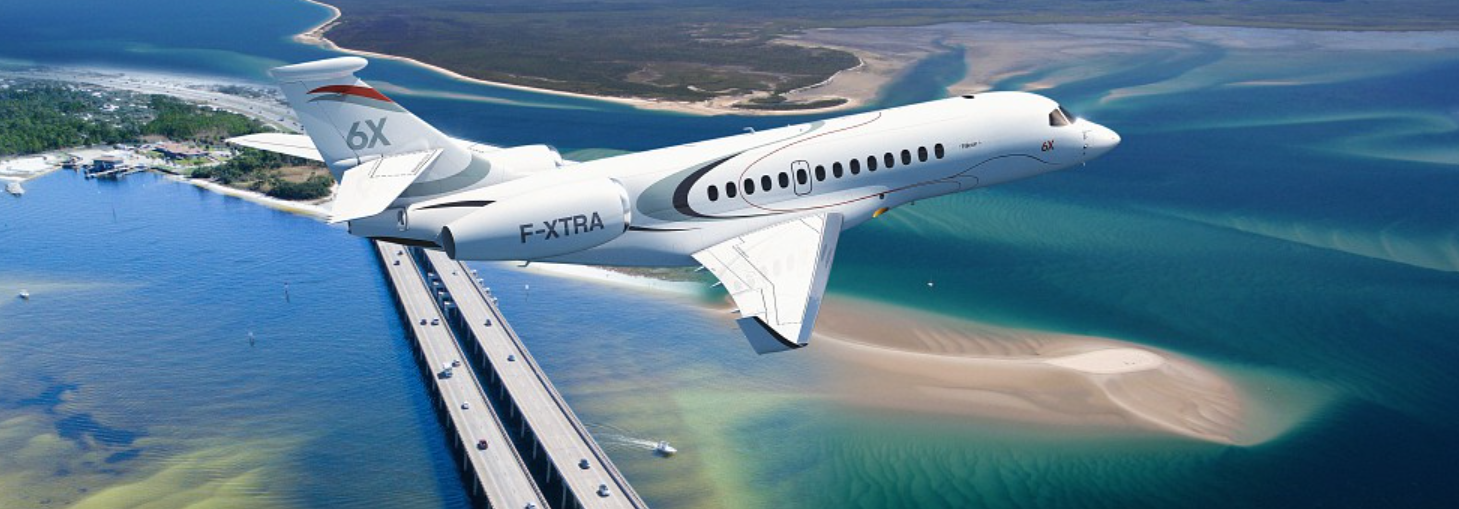
\includegraphics[width=.4\linewidth]{fig_00}
%\textit{}
}%figues de la page de garde
\def\xxtitreexo{\noindent Bateau support de ROV}
\def\xxsourceexo{\hspace{.2cm} Concours Centrale Supelec -- MP 2019}
\def\xxactivite{{Synthèse 01} \ifprof  -- Corrigé \else \fi}

%\iflivret
\input{\repRel/Style/pagegarde_TD}
%\else
%\pagestyle{empty}


%%%%%%%% PAGE DE GARDE COURS
\ifcours
\begin{tikzpicture}[remember picture,overlay]
\node at (current page.north west)
{\begin{tikzpicture}[remember picture,overlay]
\node[anchor=north west,inner sep=0pt] at (0,0) {\includegraphics[width=\paperwidth]{\thechapterimage}};
\draw[anchor=west] (-2cm,-8cm) node [line width=2pt,rounded corners=15pt,draw=ocre,fill=white,fill opacity=0.6,inner sep=40pt]{\strut\makebox[22cm]{}};
\draw[anchor=west] (1cm,-8cm) node {\huge\sffamily\bfseries\color{black} %
\begin{minipage}{1cm}
\rotatebox{90}{\LARGE\sffamily\textsc{\color{ocre}\textbf{\xxnumpartie}}}
\end{minipage} \hfill
\begin{minipage}[c]{14cm}
\begin{titrepartie}
\begin{flushright}
\renewcommand{\baselinestretch}{1.1} 
\Large\sffamily\textsc{\textbf{\xxpartie}}
\renewcommand{\baselinestretch}{1} 
\end{flushright}
\end{titrepartie}
\end{minipage} \hfill
\begin{minipage}[c]{3.5cm}
{\large\sffamily\textsc{\textbf{\color{ocre} \discipline}}}
\end{minipage} 
 };
\end{tikzpicture}};
\end{tikzpicture}


\begin{tikzpicture}[overlay]
\node[shape=rectangle, 
      rounded corners = .25 cm,
	  draw= ocre,
	  line width=2pt, 
	  fill = ocre!10,
	  minimum width  = 2.5cm,
	  minimum height = 3cm,] at (18cm,0) {};
\node at (17.7cm,0) {\rotatebox{90}{\textbf{\Large\color{ocre}{\classe}}}};
%{};
\end{tikzpicture}

\vspace{3.5cm}

\begin{tikzpicture}[remember picture,overlay]
\draw[anchor=west] (-2cm,-6cm) node {\huge\sffamily\bfseries\color{black} %
\begin{minipage}{2cm}
\begin{center}
\LARGE\sffamily\textsc{\color{ocre}\textbf{\xxactivite}}
\end{center}
\end{minipage} \hfill
\begin{minipage}[c]{15cm}
\begin{titrechapitre}
\renewcommand{\baselinestretch}{1.1} 
\Large\sffamily\textsc{\textbf{\xxnumchapitre}}

\Large\sffamily\textsc{\textbf{\xxchapitre}}
\vspace{.5cm}

\renewcommand{\baselinestretch}{1} 
\normalsize\normalfont
\xxcompetences
\end{titrechapitre}
\end{minipage}  };
\end{tikzpicture}
\vfill

\begin{flushright}
\begin{minipage}[c]{.3\linewidth}
\begin{center}
\xxfigures
\end{center}
\end{minipage}\hfill
\begin{minipage}[c]{.6\linewidth}
\startcontents
\printcontents{}{1}{}
\end{minipage}
\end{flushright}

\begin{tikzpicture}[remember picture,overlay]
\draw[anchor=west] (4.5cm,-.7cm) node {
\begin{minipage}[c]{.2\linewidth}
\begin{flushright}

\includegraphics[width=2cm]{png/logoCC}
\end{flushright}
\end{minipage}
\begin{minipage}[c]{.2\linewidth}
\textsl{\xxauteur} \\
\textsl{\classe}
\end{minipage}
 };
\end{tikzpicture}
\newpage
\pagestyle{fancy}

\newpage
\pagestyle{fancy}

\else
\fi


%%%%%%%% PAGE DE GARDE TD
\iftd
%\begin{tikzpicture}[remember picture,overlay]
%\node at (current page.north west)
%{\begin{tikzpicture}[remember picture,overlay]
%\draw[anchor=west] (-2cm,-3.25cm) node [line width=2pt,rounded corners=15pt,draw=ocre,fill=white,fill opacity=0.6,inner sep=40pt]{\strut\makebox[22cm]{}};
%\draw[anchor=west] (1cm,-3.25cm) node {\huge\sffamily\bfseries\color{black} %
%\begin{minipage}{1cm}
%\rotatebox{90}{\LARGE\sffamily\textsc{\color{ocre}\textbf{\xxnumpartie}}}
%\end{minipage} \hfill
%\begin{minipage}[c]{13.5cm}
%\begin{titrepartie}
%\begin{flushright}
%\renewcommand{\baselinestretch}{1.1} 
%\Large\sffamily\textsc{\textbf{\xxpartie}}
%\renewcommand{\baselinestretch}{1} 
%\end{flushright}
%\end{titrepartie}
%\end{minipage} \hfill
%\begin{minipage}[c]{3.5cm}
%{\large\sffamily\textsc{\textbf{\color{ocre} \discipline}}}
%\end{minipage} 
% };
%\end{tikzpicture}};
%\end{tikzpicture}

%%%%%%%%%% PAGE DE GARDE TD %%%%%%%%%%%%%%%
%\begin{tikzpicture}[overlay]
%\node[shape=rectangle, 
%      rounded corners = .25 cm,
%	  draw= ocre,
%	  line width=2pt, 
%	  fill = ocre!10,
%	  minimum width  = 2.5cm,
%	  minimum height = 2.5cm,] at (18.5cm,0) {};
%\node at (17.7cm,0) {\rotatebox{90}{\textbf{\Large\color{ocre}{\classe}}}};
%%{};
%\end{tikzpicture}

% PARTIE ET CHAPITRE
%\begin{tikzpicture}[remember picture,overlay]
%\draw[anchor=west] (-1cm,-2.1cm) node {\large\sffamily\bfseries\color{black} %
%\begin{minipage}[c]{15cm}
%\begin{flushleft}
%\xxnumchapitre \\
%\xxchapitre
%\end{flushleft}
%\end{minipage}  };
%\end{tikzpicture}

% Bandeau titre exo
\begin{tikzpicture}[remember picture,overlay]
\draw[anchor=west] (-2cm,-6cm) node {\huge\sffamily\bfseries\color{black} %
\begin{minipage}{5cm}
\begin{center}
\LARGE\sffamily\color{ocre}\textbf{\textsc{\xxactivite}}

\begin{center}
\xxfigures
\end{center}

\end{center}
\end{minipage} \hfill
\begin{minipage}[c]{12cm}
\begin{titrechapitre}
\renewcommand{\baselinestretch}{1.1} 
\large\sffamily\textbf{\textsc{\xxtitreexo}}

\small\sffamily{\textbf{\textit{\color{black!70}\xxsourceexo}}}
\vspace{.5cm}

\renewcommand{\baselinestretch}{1} 
\normalsize\normalfont
\xxcompetences
\end{titrechapitre}
\end{minipage}  };
\end{tikzpicture}

\else
\fi


%%%%%%%% PAGE DE GARDE FICHE
\iffiche
\begin{tikzpicture}[remember picture,overlay]
\node at (current page.north west)
{\begin{tikzpicture}[remember picture,overlay]
\draw[anchor=west] (-2cm,-3.25cm) node [line width=2pt,rounded corners=15pt,draw=ocre,fill=white,fill opacity=0.6,inner sep=40pt]{\strut\makebox[22cm]{}};
\draw[anchor=west] (1cm,-3.25cm) node {\huge\sffamily\bfseries\color{black} %
\begin{minipage}{1cm}
\rotatebox{90}{\LARGE\sffamily\textsc{\color{ocre}\textbf{\xxnumpartie}}}
\end{minipage} \hfill
\begin{minipage}[c]{14cm}
\begin{titrepartie}
\begin{flushright}
\renewcommand{\baselinestretch}{1.1} 
\large\sffamily\textsc{\textbf{\xxpartie} \\} 

\vspace{.2cm}

\normalsize\sffamily\textsc{\textbf{\xxnumchapitre -- \xxchapitre}}
\renewcommand{\baselinestretch}{1} 
\end{flushright}
\end{titrepartie}
\end{minipage} \hfill
\begin{minipage}[c]{3.5cm}
{\large\sffamily\textsc{\textbf{\color{ocre} \discipline}}}
\end{minipage} 
 };
\end{tikzpicture}};
\end{tikzpicture}


\begin{tikzpicture}[overlay]
\node[shape=rectangle, 
      rounded corners = .25 cm,
	  draw= ocre,
	  line width=2pt, 
	  fill = ocre!10,
	  minimum width  = 2.5cm,
%	  minimum height = 2.5cm,] at (18.5cm,0.5cm) {};
	  minimum height = 2.5cm,] at (18.5cm,0cm) {};
\node at (17.7cm,0) {\rotatebox{90}{\textsf{\textbf{\large\color{ocre}{\classe}}}}};
%{};
\end{tikzpicture}



\else
\fi



%\fi

\setlength{\columnseprule}{.1pt}

\pagestyle{fancy}
\thispagestyle{plain}

\vspace{4.5cm}

\def\columnseprulecolor{\color{bleuxp}}
\setlength{\columnseprule}{0.4pt} 
\setcounter{numques}{0}
%%%%%%%%%%%%%%%%%%%%%%%


\ifprof
\else
\begin{multicols}{2}
\fi
\section*{Introduction}
\ifprof
\else
On s'intéresse à une grue permettant la dépose sur fond marin d'un robot dont l'objectif est d'enfouir des câbles.
\fi
%
%\section{Introduction}
%\ifprof
%\else
%Le développement de fermes éoliennes en mer nécessite la pose de câbles sous-marins de forte puissance sur de très
%grandes distances. Le déploiement de ces câbles doit se faire en tenant compte de contraintes environnementales
%sévères visant à limiter l’impact sur le milieu marin. Les opérateurs « offshore » ont constaté une élévation
%de la température de l’eau autour du câble provoquant le développement de micro-organismes. Pour limiter ce
%phénomène, la solution est d’ensouiller (enfouir) le câble dans les sédiments terrigènes des plateaux continentaux.
%La société TravOcéan a acquis au fil des années une expertise unique dans les domaines de la pose et de la
%protection de câbles sous-marins, couvrant en particulier tous les types de sol (du sol très meuble au sol très
%dur) ainsi que tous les types de câbles (fibre optique, câbles électriques).
%
%\begin{figure}[H]
%\centering
%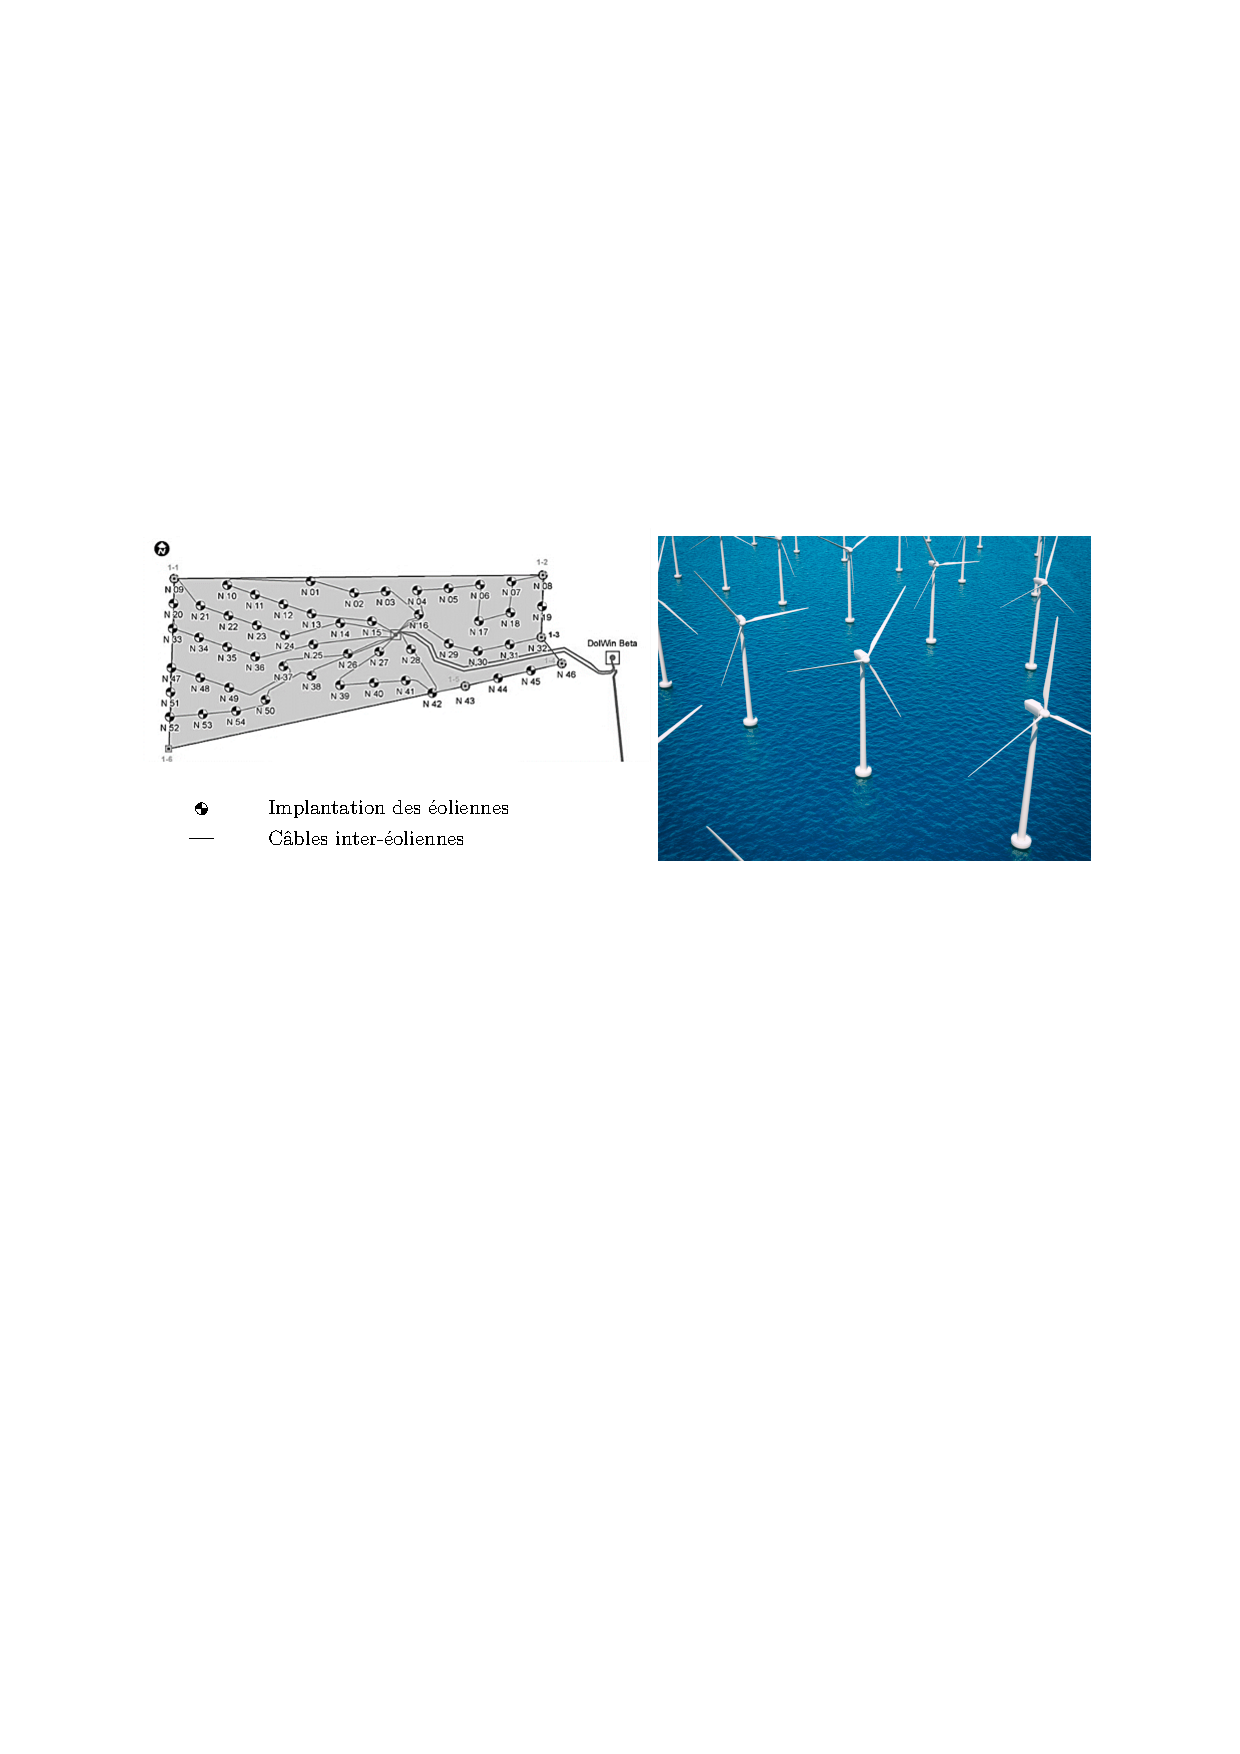
\includegraphics[width=0.85\linewidth]{Fig1}
%\caption{Implantation de la ferme éolienne North See One}
%\label{Fig1}
%\end{figure}
%
%
%
%
%Pour réaliser l’ensouillage, le câble est déposé sur le fond marin par un navire câblier. Le robot sous-marin ROV
%(Remotely Operated Vehicle) est déposé sur le fond marin par un bateau support et ensouille le câble provenant
%du navire câblier après l’avoir détecté et s’être aligné dans l’axe de celui-ci (\autoref{Fig2}).
%
%\begin{figure}[H]
%\centering
%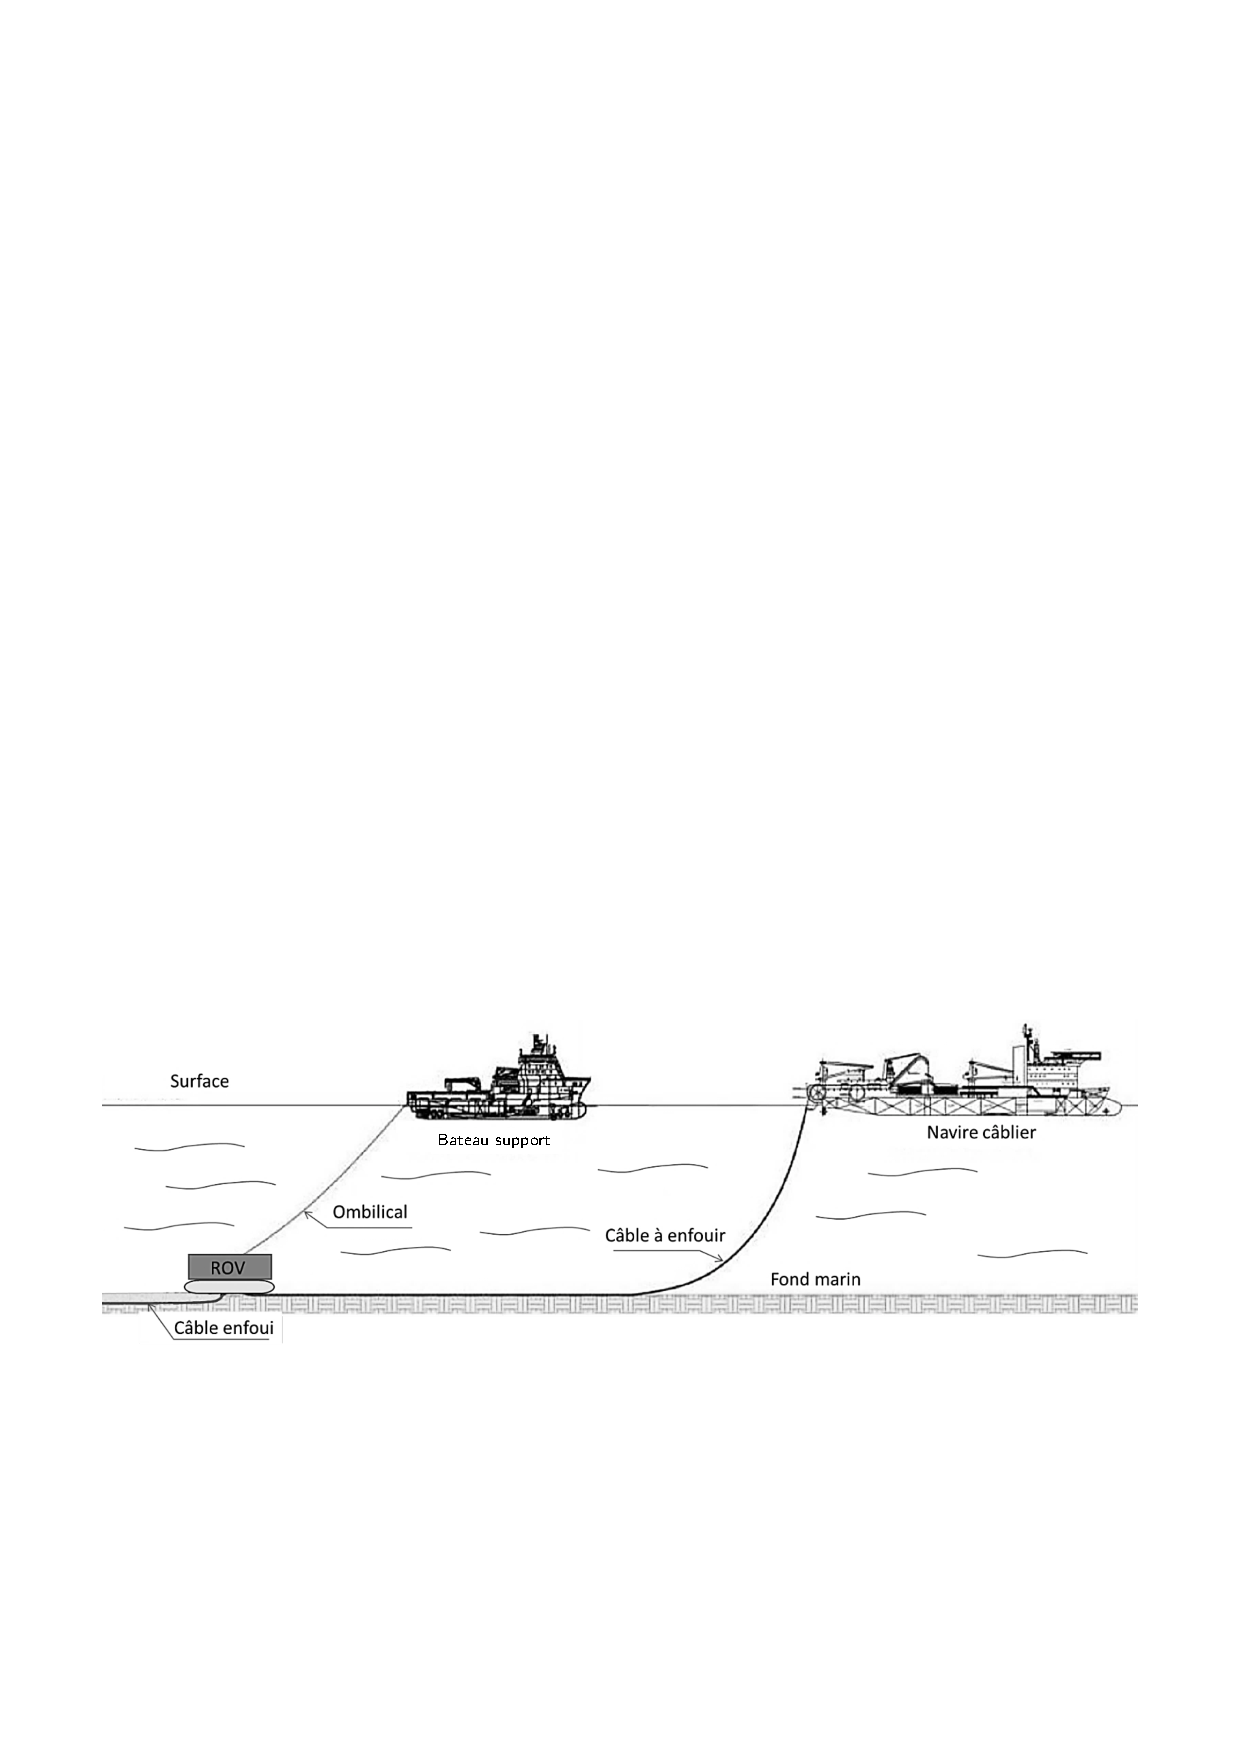
\includegraphics[width=0.85\linewidth]{Fig2}
%\caption{Environnement du ROV}
%\label{Fig2}
%\end{figure}
%
%
%
%
%Les opérations de mise en \oe{}uvre du ROV se font en trois étapes.
%\begin{itemize}
%\item \textbf{Étape 1.} Mise à l’eau
%Cette phase utilise une grue portique pour transférer le ROV du pont du bateau support jusqu’à
%l’aplomb de la surface d’immersion. Dans cette phase, le ROV n’est porté par aucun câble mais par
%un dispositif d’accrochage spécifique appelé snubber (\autoref{Fig3}).
%\item \textbf{Étape 2.} Descente
%Dans cette phase, le ROV est suspendu à un câble ombilical. Un bon équilibrage hydrostatique est
%nécessaire pour assurer l’horizontalité du ROV pendant la descente.
%\item \textbf{Étape 3.} Enfouissement du câble. Non étudié dans ce sujet.
%\end{itemize}
%

\ifprof
\else
\begin{figure}[H]
\centering
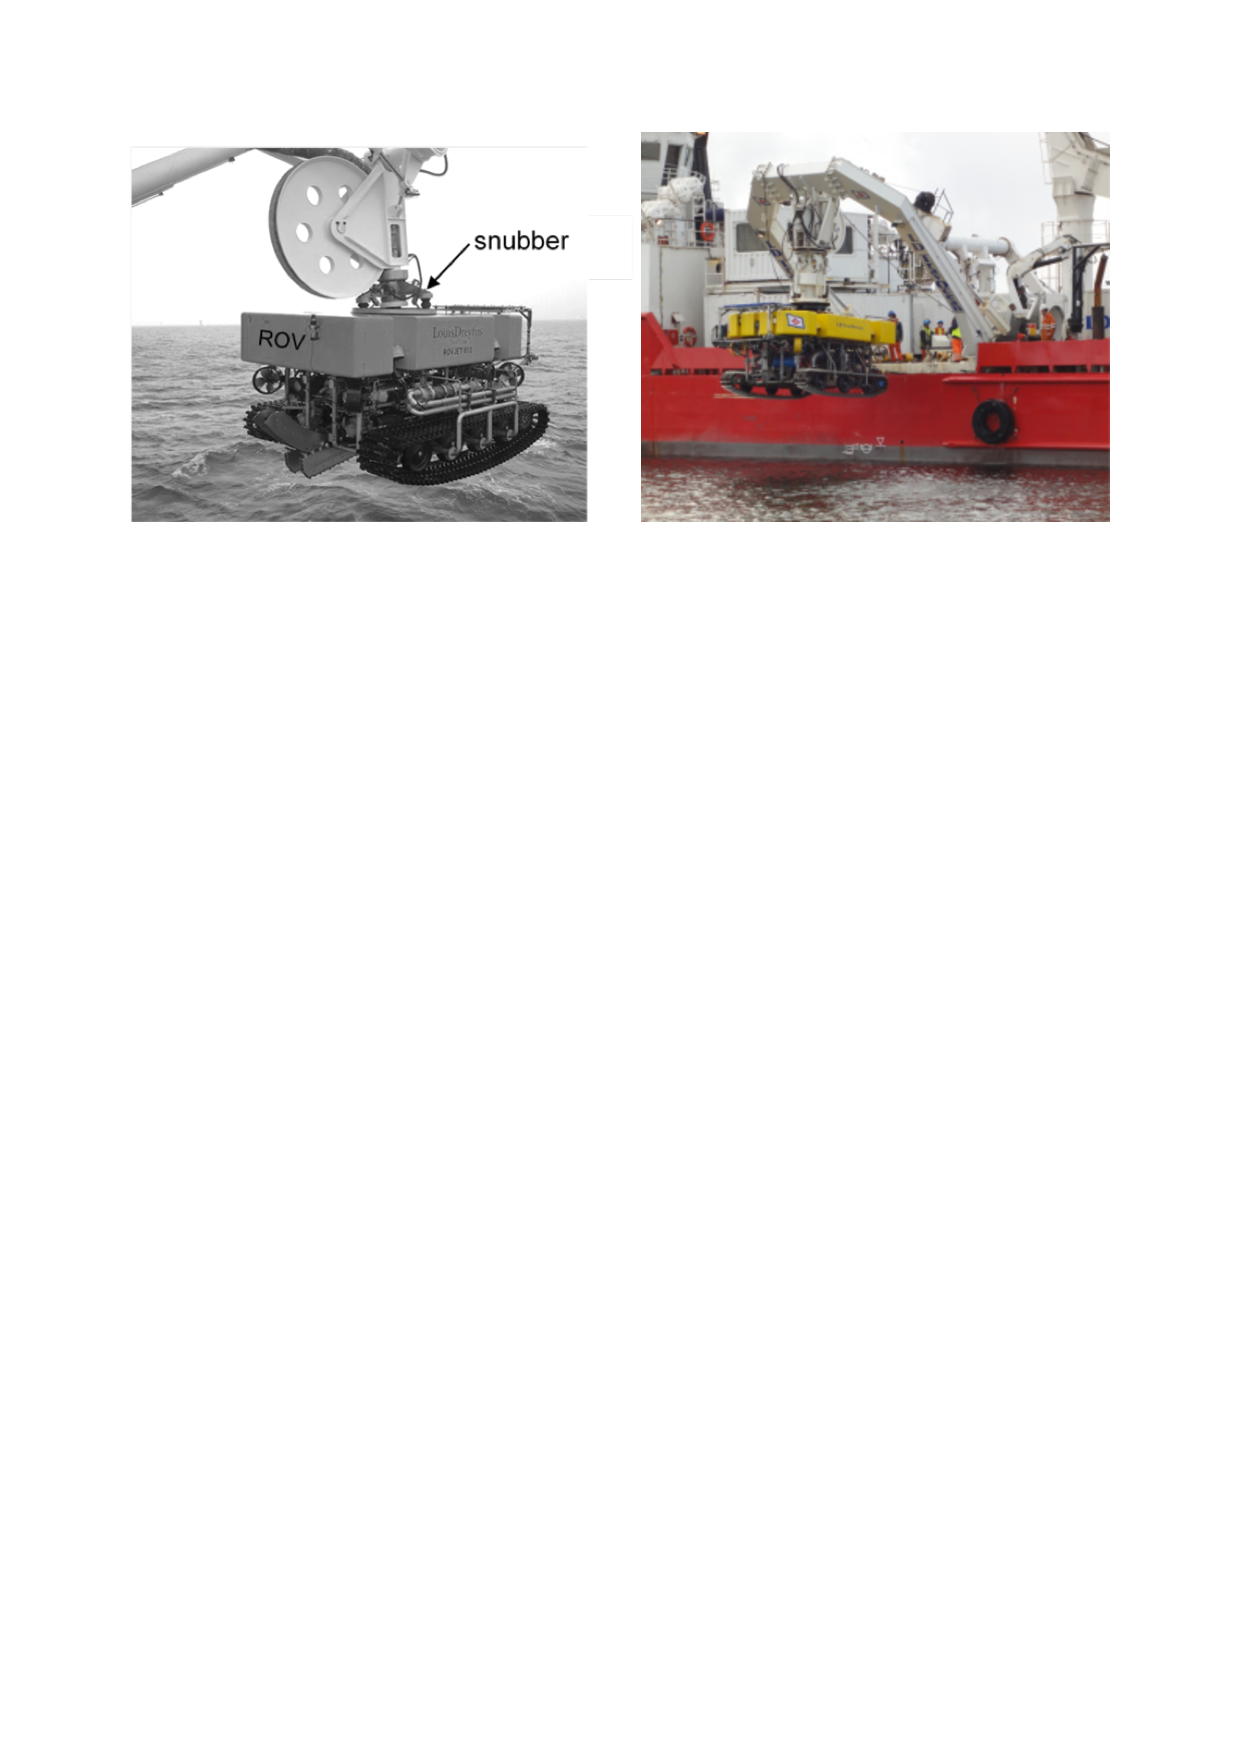
\includegraphics[width=0.85\linewidth]{Fig3}
\caption{ROV suspendu à la grue portique}
\label{Fig3}
\end{figure}
\fi



%\textbf{Objectif} %
\begin{obj}
Vérifier si le bateau support est capable de limiter suffisamment les effets de la houle.
\end{obj}


\ifprof
\else
La société TravOcéan souhaite pouvoir travailler dans des conditions de mer difficiles pour limiter au maximum
les périodes d’arrêt des chantiers. Pour cela, elle souhaite disposer d’un système de treuillage de ses ROV
certifié pour une houle d’amplitude verticale de \SI{5}{m}. Le tableau suivant 
%\autoref{tab1} 
présente un extrait du cahier des charges correspondant.

%\begin{table}[htp]
\footnotesize
\begin{center}
\begin{tabular}{|p{3cm}|p{2cm}|p{2cm}|}
\hline
\textbf{Exigence} &\textbf{Critère}& \textbf{Niveau}\\
\hline
\hline
Id 1.1&&\\
Compensation des mouvements du&Amplitude verticale du ROV&< 1 m pour 5 m d’amplitude de\\
ROV pour une houle d’amplitude&maximale&houle\\
de 5 m et de pulsations comprises&&\\
entre $0,5 \ \text{rad}\cdot \text s^{-1}$ à $1,7 \ \text{rad}\cdot \text s^{-1}$&&\\
\hline
Id 1.2&&\\
Mise en tension du câble &Temps de réponse, $t_{r5\%}$ & $< 3$ s \\
\hline
\end{tabular}

\textit{Extrait du cahier des charges}
\label{tab1}
\end{center}

\normalsize

%\end{table}

Une étude expérimentale en bassin de carène a permis d’obtenir un modèle de comportement de l’ensemble
$S =$ \{bateau + portique + ROV\} suivant l’axe vertical, sous l’effet de la houle, au point d’ancrage du ROV sur
la grue portique.\\

La fonction de transfert de l’ensemble $S$ est $B(p) =\dfrac{Y_S(p)}{Y_{\text{vague}}(p)}$ avec $Y_S(p)$ la transformée de Laplace de la variation
du déplacement vertical du point d’ancrage du ROV et $Y_{\text{vague}}(p)$ la transformée de Laplace de la variation du déplacement de la surface de l’eau à la verticale du point d’ancrage du ROV.\\

\fi


\question{ Rappeler la définition du gain en décibel. En déduire la valeur en décibel traduisant l’exigence ~Id 1.1.}

\ifprof
\begin{corrige}

La définition du gain en décibel de la fonction de transfert $B(j\omega)$ est $G_{\text{dB}}(\omega)=20\log \left \vert \dfrac{Y_S(j\omega)}{Y_{\text{vague}}(j\omega)}\right \vert$. L'exigence Id 1.1 impose une amplitude maximale du ROV de 1 m pour 5 m de houle soit :
$$\boxed{G_{\text{dB}(\omega)}<20 \log \dfrac{1}{5}\approx - 14 \ \text{dB} \ \ \forall \ \ \omega\in[0,5;1,7]  \ \text{rad/s}.}$$
\end{corrige}
\else
\fi

\ifprof
\else
Le tracé du gain de $B(p)$ dans la figure suivante.



\begin{center}
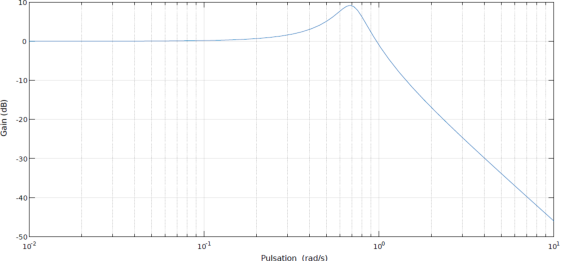
\includegraphics[width=\linewidth]{DR_A}
%\caption{ROV suspendu à la grue portique}
%\label{Fig3}
\end{center}

\fi


\question{En faisant apparaître le domaine d’utilisation, montrer que le système ne répond pas à l’exigence d’atténuation d’une houle de \SI{5}{m}.}%Répondre entièrement à cette question sur le document réponse. }
\ifprof
\begin{corrige}
%\textbf{Q2}   
On observe un phénomène de résonance, le système amplifie la houle entre 0,5 et 1 rad/s et l’atténue à une valeur maximale de 13-14 dB pour 1,7 rad/s. Le syst\`eme ne répond donc pas \`a l’exigence d'atténuation d'une houle de 5 m.
\begin{figure}[H]
\centering
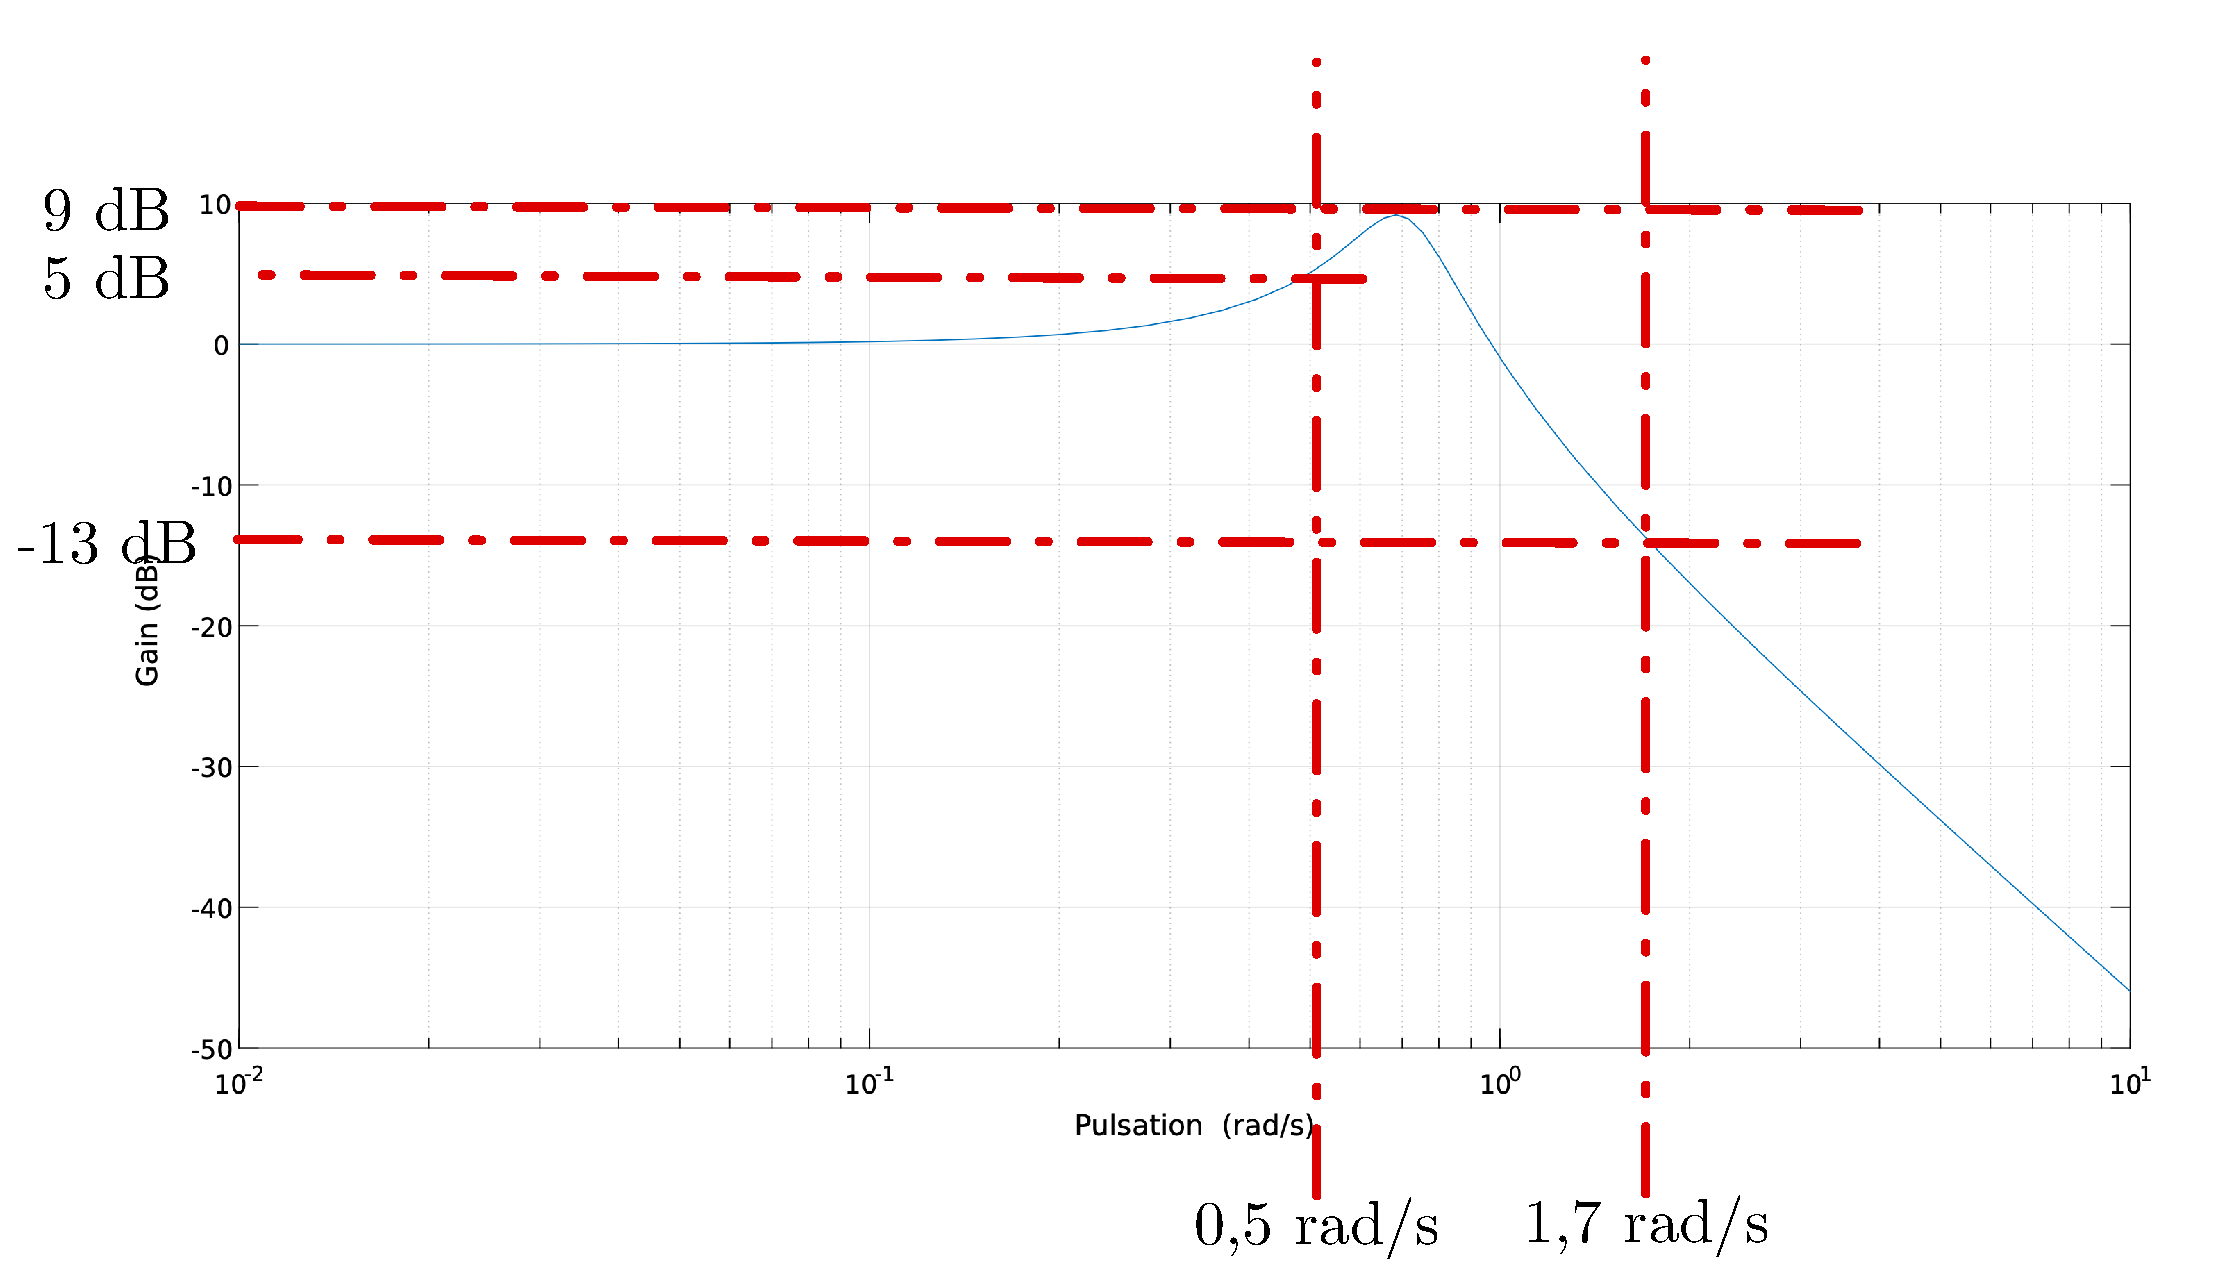
\includegraphics[width=0.65\linewidth]{Q2}
\end{figure}


\end{corrige}
\else
\fi




%
%\subsection{Conclusion}
%L’analyse du comportement du bateau sous l’effet de la houle montre que les conditions ne sont pas réunies
%pour travailler par une houle de 5 m. La société TravOcéan doit donc répondre à la problématique suivante :
%\textit{comment assurer le transfert du ROV entre le bateau support et l’océan dans les conditions définies
%par la norme « Cranes and Submersibles Lifting Appliances » pour une amplitude de houle de 5 m en
%toute sécurité pour l’environnement, les opérateurs et le matériel ?}


%\section{Transfert du ROV : étude de l’actionneur de mise à l’eau}
%
%%\textbf{Objectif} 
%\begin{obj}
%Vérifier le dimensionnement du vérin de la grue portique permettant la mise à l’eau du ROV en
%respectant la norme « Cranes and Submersibles Lifting Appliances ».
%\end{obj}
%\ifprof
%\else
%
%Le câble ombilical est enroulé sur un tambour motorisé équipé d’un système de trancannage (%\footnote{
%Le trancannage est une opération de va-et-vient nécessaire au bon enroulement d’un câble sur un tambour.)%} (\autoref{Fig4}). Il est
%raccordé au ROV par un snubber de jonction. La grue portique est actionnée par un ensemble de deux vérins
%hydrauliques modélisés en un seul vérin équivalent pour cette étude.
%
%
%\begin{figure}[H]
%\centering
%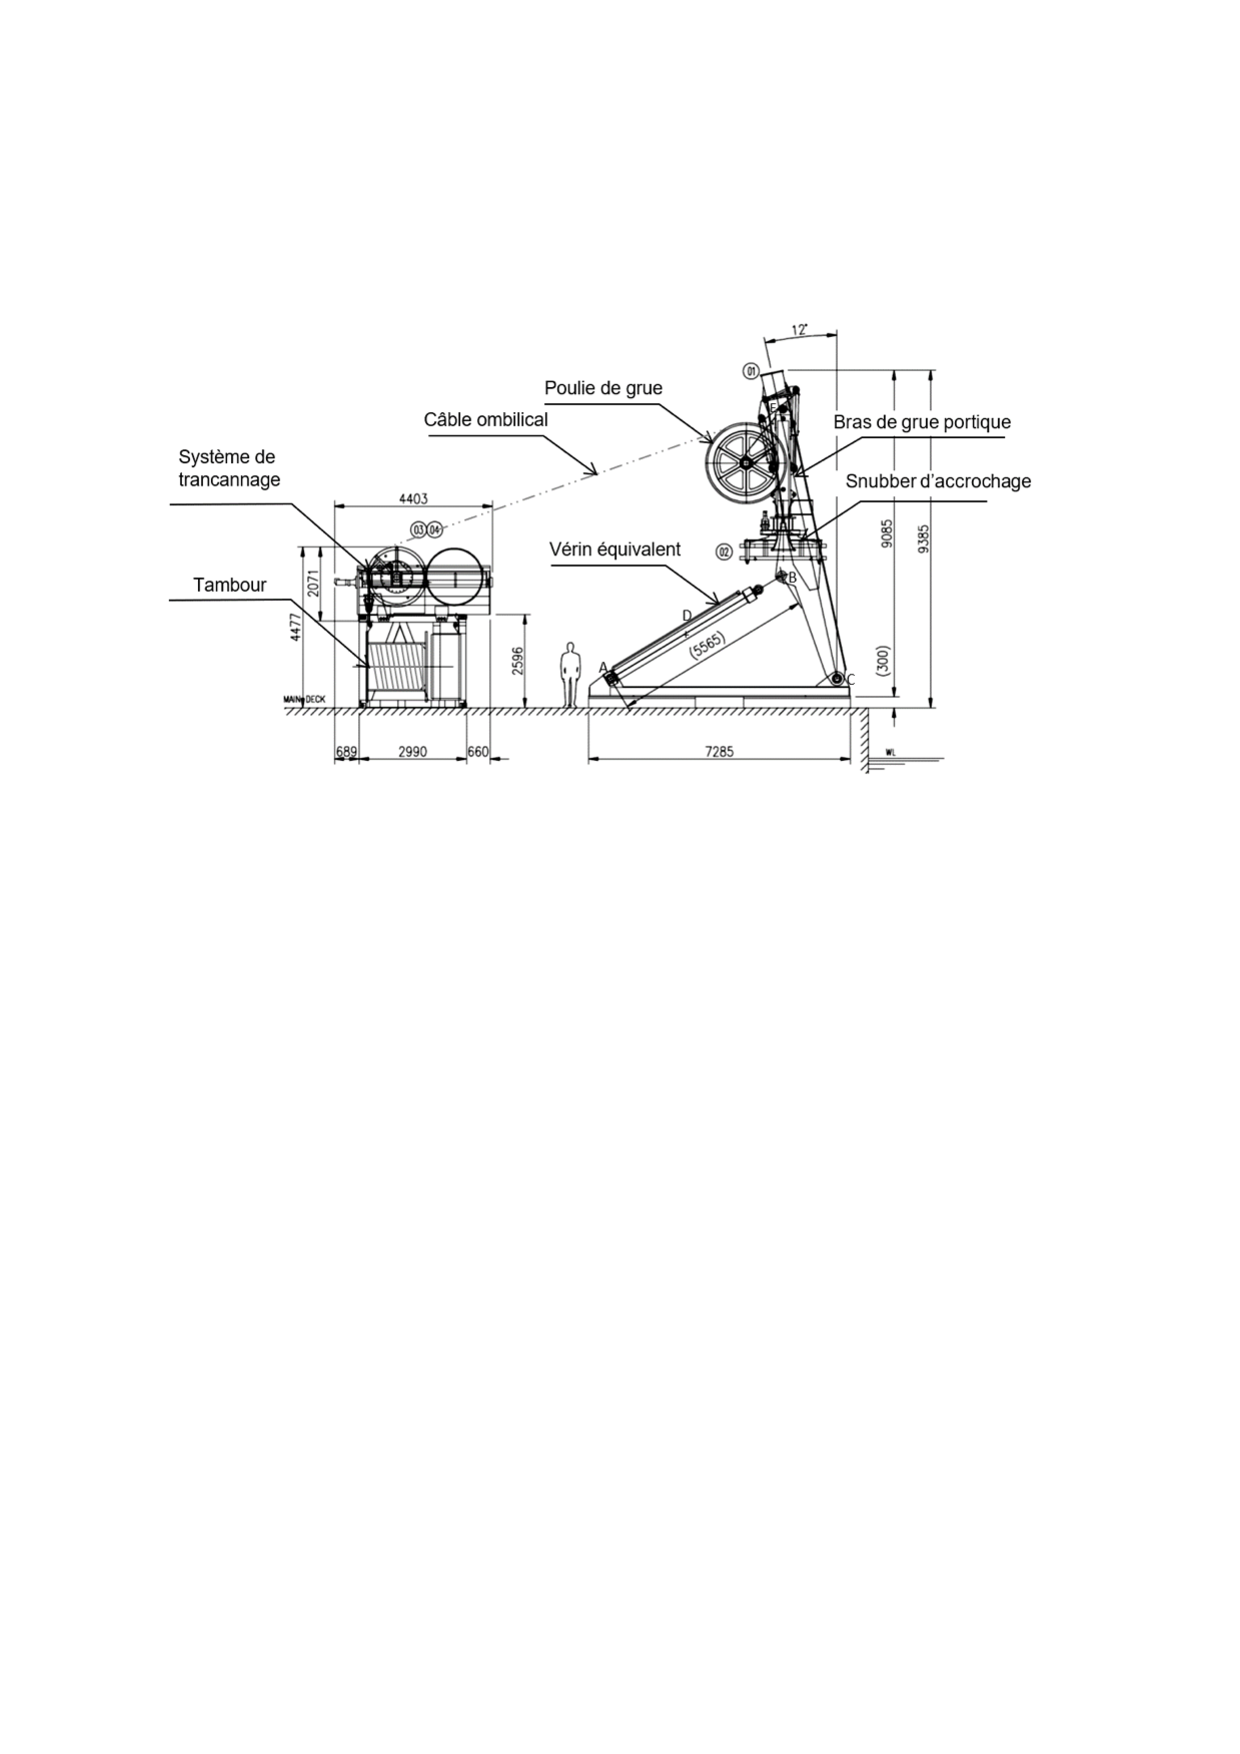
\includegraphics[width=0.85\linewidth]{Fig4}
%\caption{ Implantation de la grue et du tambour d’enroulement sur le pont du bateau}
%\label{Fig4}
%\end{figure}
%
%
%Les conditions de houle et la masse importante du ROV (13 tonnes) impliquent un dimensionnement précis
%des éléments définis par la norme de certification « Cranes and Submersibles Lifting Appliances » qui impose
%des coefficients de majoration pour prendre en compte des effets dynamiques dus à une houle donnée. La grue
%portique et les éléments de levage sont conçus pour être homologués avec une houle de 5 m.
%Conditions d’étude :
%\begin{itemize}
%\item d’après la norme, les effets de la houle impliquent une majoration de 100\% des efforts statiques ;
%\item \textbf{attention, erreur de signe dans le sujet d'origine.} Le portique se déplace entre $-12^\circ$ et $53^\circ$ par rapport à la verticale (\autoref{Fig5}).
%\end{itemize}
%
%\begin{figure}[H]
%\centering
%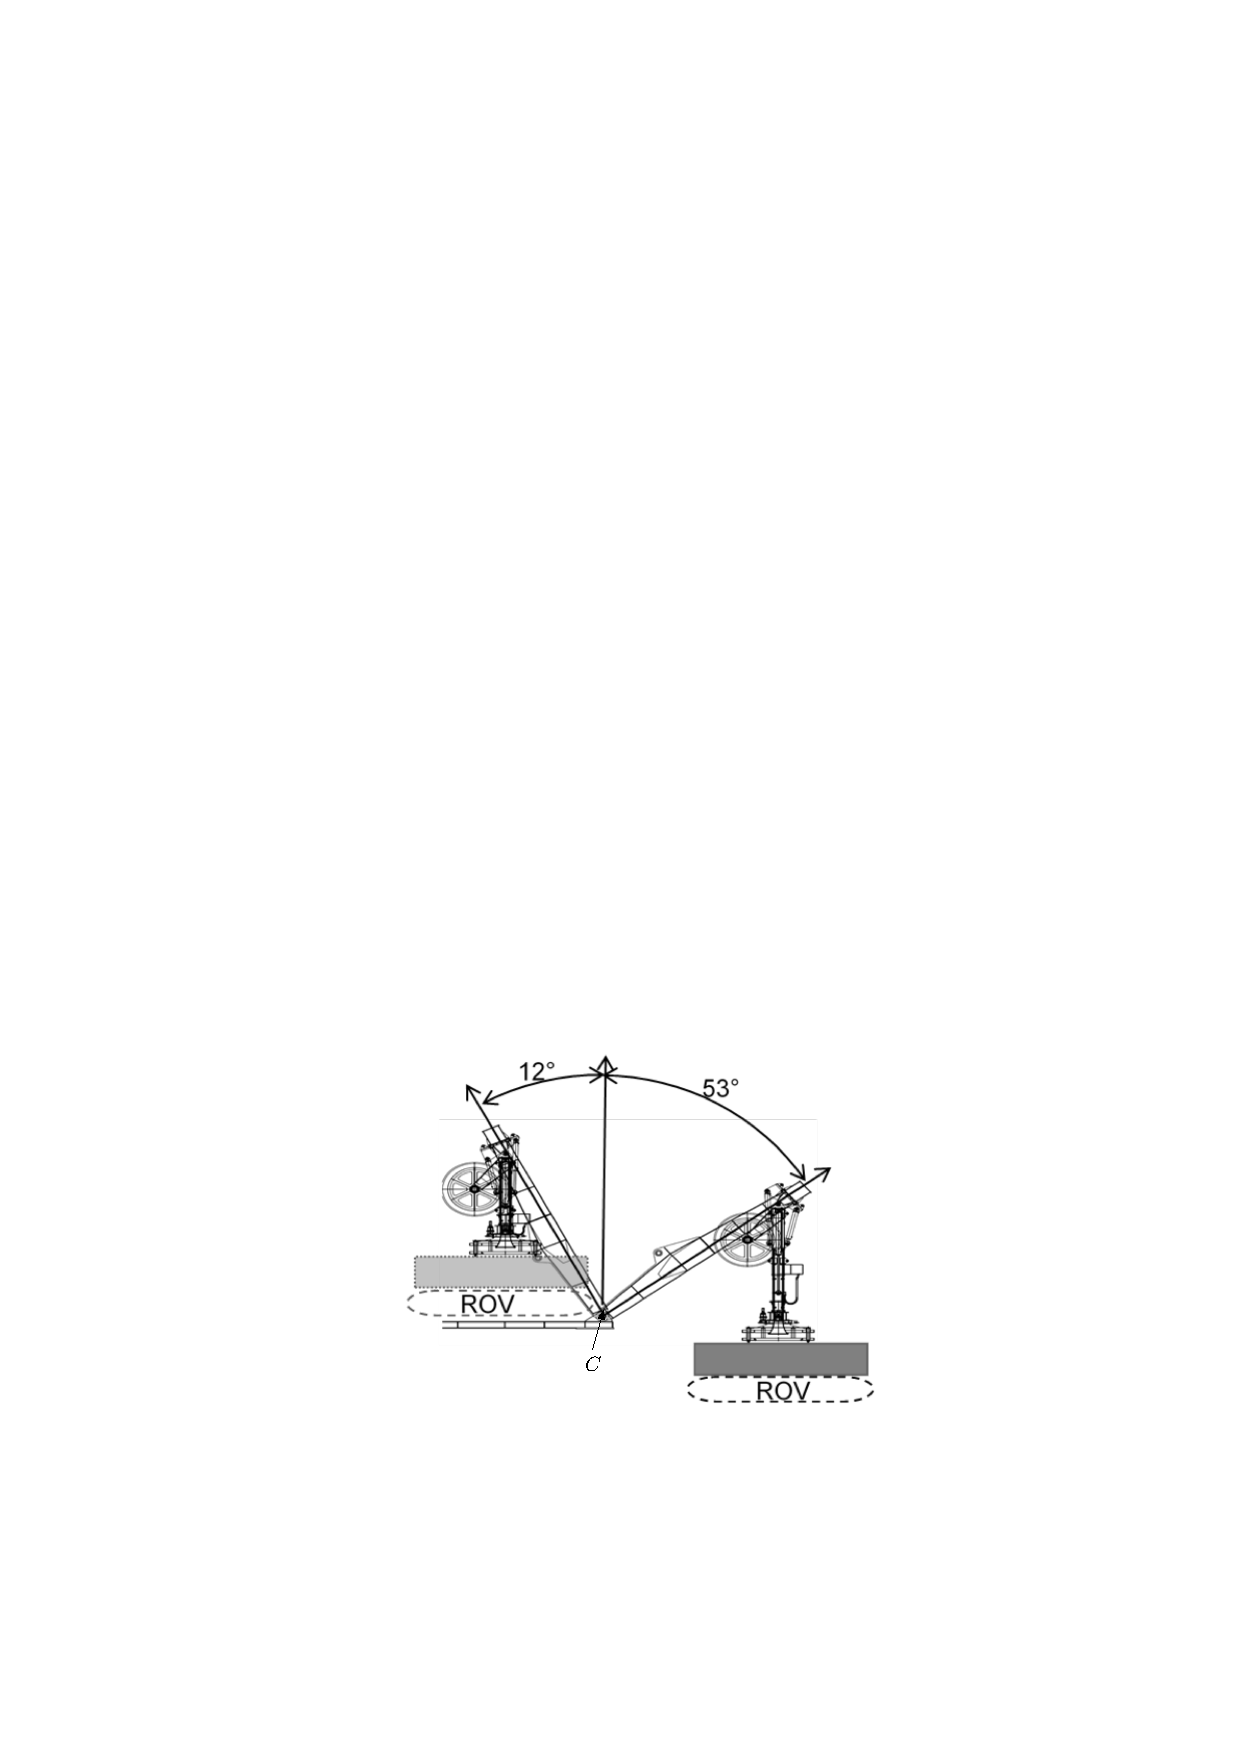
\includegraphics[width=0.4\linewidth]{Fig5}
%\caption{Positions extrêmes du ROV}
%\label{Fig5}
%\end{figure}
%
%
%
%
%La grue portique permet le transfert du ROV entre la surface de l’eau et le bateau support. Dans cette phase
%le ROV est relié au snubber (\autoref{Fig5}). Le câble n’est pas porteur.
%
%
%
%On souhaite déterminer la course et les efforts dans les vérins pour vérifier que la pression du groupe hydraulique
%d’alimentation disponible sur le bateau support est suffisante et que la géométrie choisie est correctement
%dimensionnée.
%Pour cette étude le constructeur a fait les hypothèses suivantes :
%\begin{itemize}
%\item les liaisons sont considérées comme parfaites ;
%\item les liaisons pivot en $A$ et $B$ seront modélisées par des rotules pour l’étude des efforts ;
%\item l’action du snubber, sur lequel est fixé le ROV, sur le bras de la grue portique est modélisée par un torseur
%exprimé en $E$, $$\begin{Bmatrix}\overrightarrow{F}_{\text{ROV}\to \text{bras}}=-Mg\overrightarrow{y_0}\\ \overrightarrow{0}\end{Bmatrix}_E,$$ avec $M = 13 000$ kg ;
%\item le poids des pièces autres que le ROV est supposé négligeable devant les autres efforts mis en jeu ;
%\item le repère $\mathcal R_0(C, \overrightarrow{x_0},\overrightarrow{y_0},\overrightarrow{z_0})$ est supposé galiléen.
%\end{itemize}
%
%
%\begin{figure}[H]
%\centering
%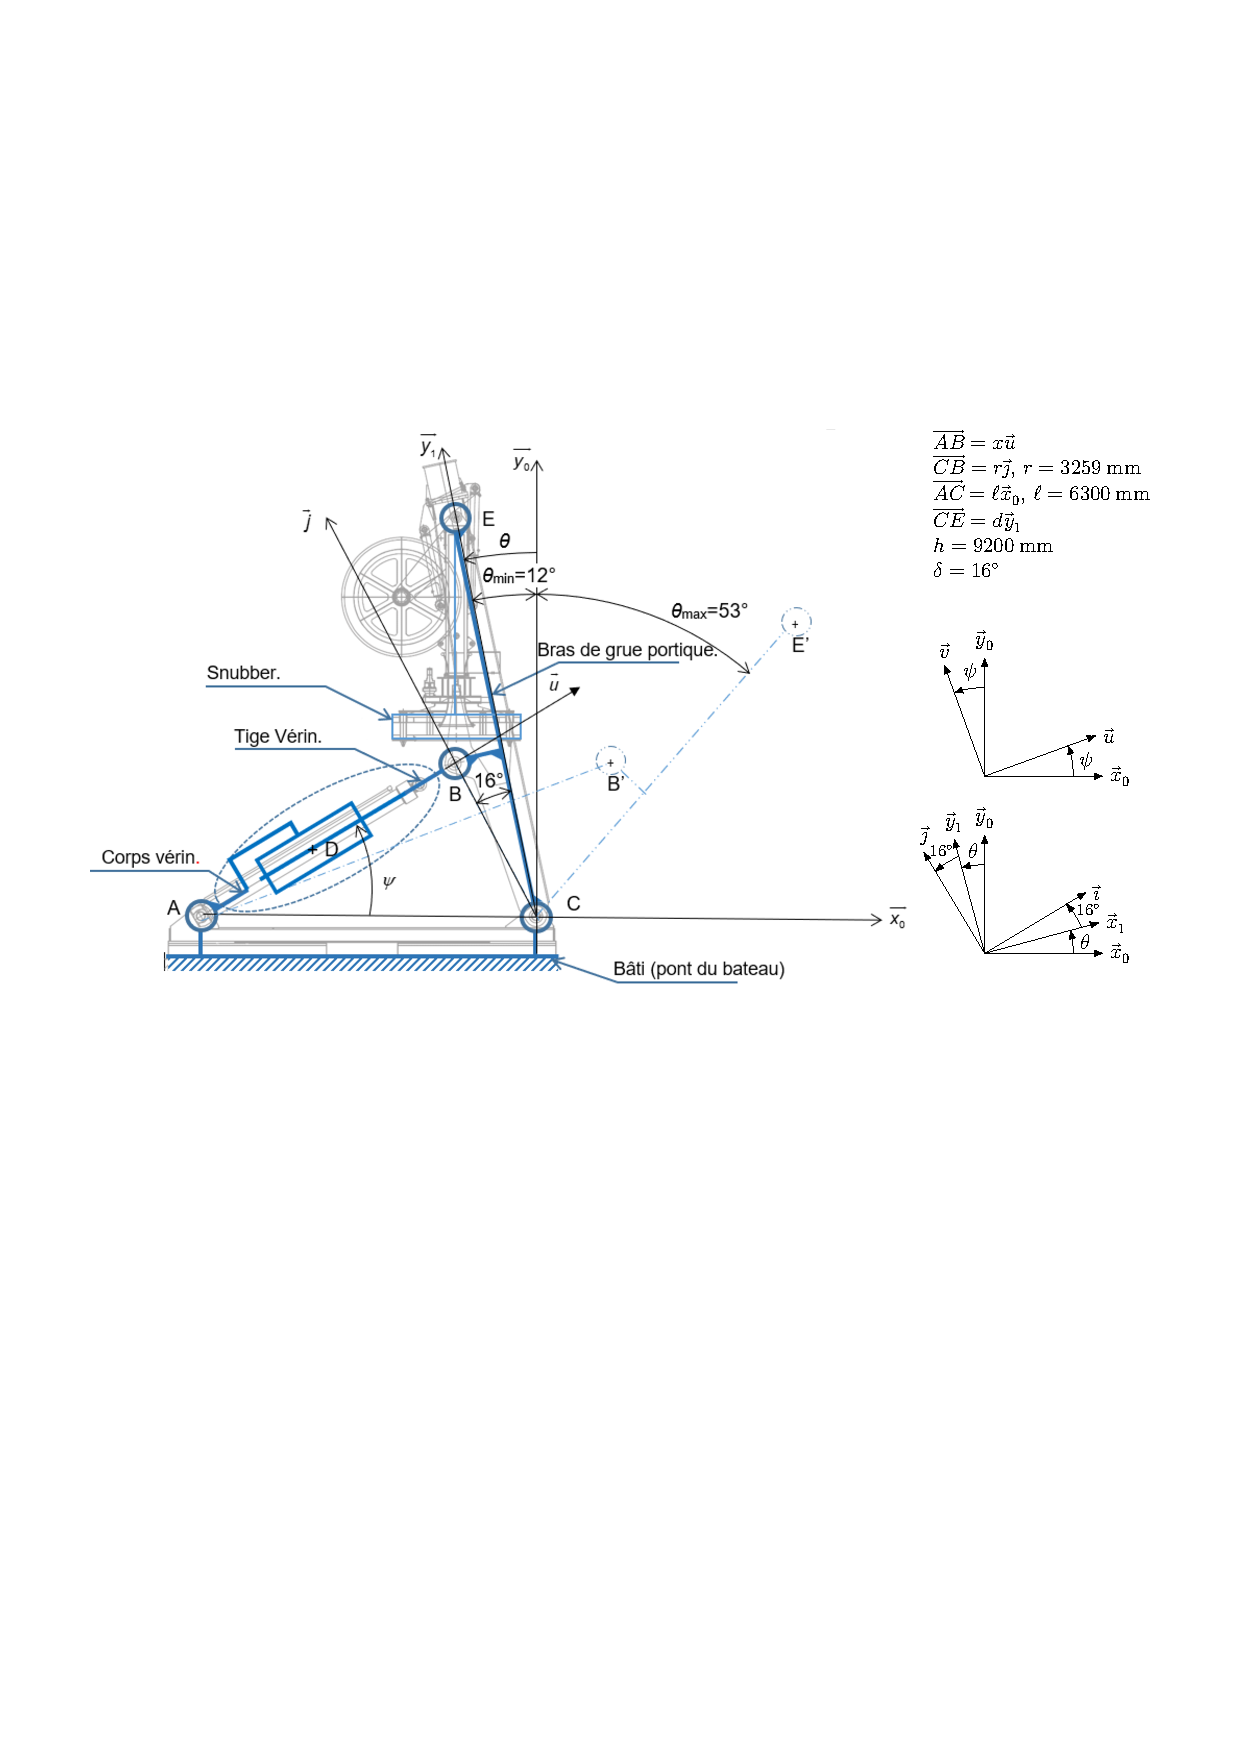
\includegraphics[width=0.85\linewidth]{Fig6}
%\caption{Schéma cinématique de la grue portique  \textbf{Erreur de notation : $d=h=CE$}}
%\label{Fig6}
%\end{figure}
%
%
%
%
%Une modélisation 3D du bras de la grue portique et du vérin principal a permis d’obtenir un modèle mécanique
%à utiliser par la suite dans le modèle multiphysique de simulation.\\
%
%\fi
%
%\question{Déterminer la loi entrée sortie $x = f(\theta, r, l, \delta)$ par une fermeture géométrique à partir des données du schéma cinématique.}
%
%\ifprof
%\begin{corrige}
%
%  On effectue une fermeture géometrique sur la chaine fermée de solides 0-1-2-3-0. On obtient :
%\begin{eqnarray}
%\overrightarrow{AB}+\overrightarrow{BC}+\overrightarrow{CA}&=&\overrightarrow{0},\nonumber\\
%x\overrightarrow{u}-r\overrightarrow{j}-l\overrightarrow{x_0}&=&\overrightarrow{0}.\nonumber
%\end{eqnarray}
%
%On projette la dernière équation dans le repère $\mathcal R_0$ et on obtient :
%\begin{eqnarray}
%x\cos \psi + r\sin(\theta+\delta)-l&=&0,\nonumber\\
%x\sin \psi - r\cos(\theta+\delta)&=&0.\nonumber
%\end{eqnarray}
%
%On obtient :
%$$\boxed{x=\sqrt{(r\sin(\theta+\delta)-l)^2+r^2\cos^2(\theta+\delta)}=\sqrt{r^2+l^2-2lr\sin(\theta+\delta)}.}$$
%
%\end{corrige}
%\else
%\fi
%
%
%\question{En déduire, en justifiant les calculs, l’expression littérale et la valeur numérique de la course $c$ du vérin.}
%
%\ifprof
%\begin{corrige}
%%\textbf{Q4}  
%\textcolor{red}{Remarque : erreur dans l’énoncé, les signes des angles sont inversés. Selon les figures, le portique se déplace entre $-53^\circ$ et $+12^\circ$.} \\
%
%La course du vérin est $c=x_{\text{max}}-x_{\text{min}}=x(\theta=-52^\circ)-x(\theta=+12^\circ)$ donc :
%
%$$\boxed{c\approx 3091 \ \text{mm}.}$$ 
%
%\textcolor{red}{Ci-dessous le tracé issu de la fermeture géométrique sur la plage [$-53^\circ$;$+12^\circ$] et la Figure 6 modifiée (angles et données géométriques, $d=h$).}
%
%\begin{figure}[H]
%\centering
%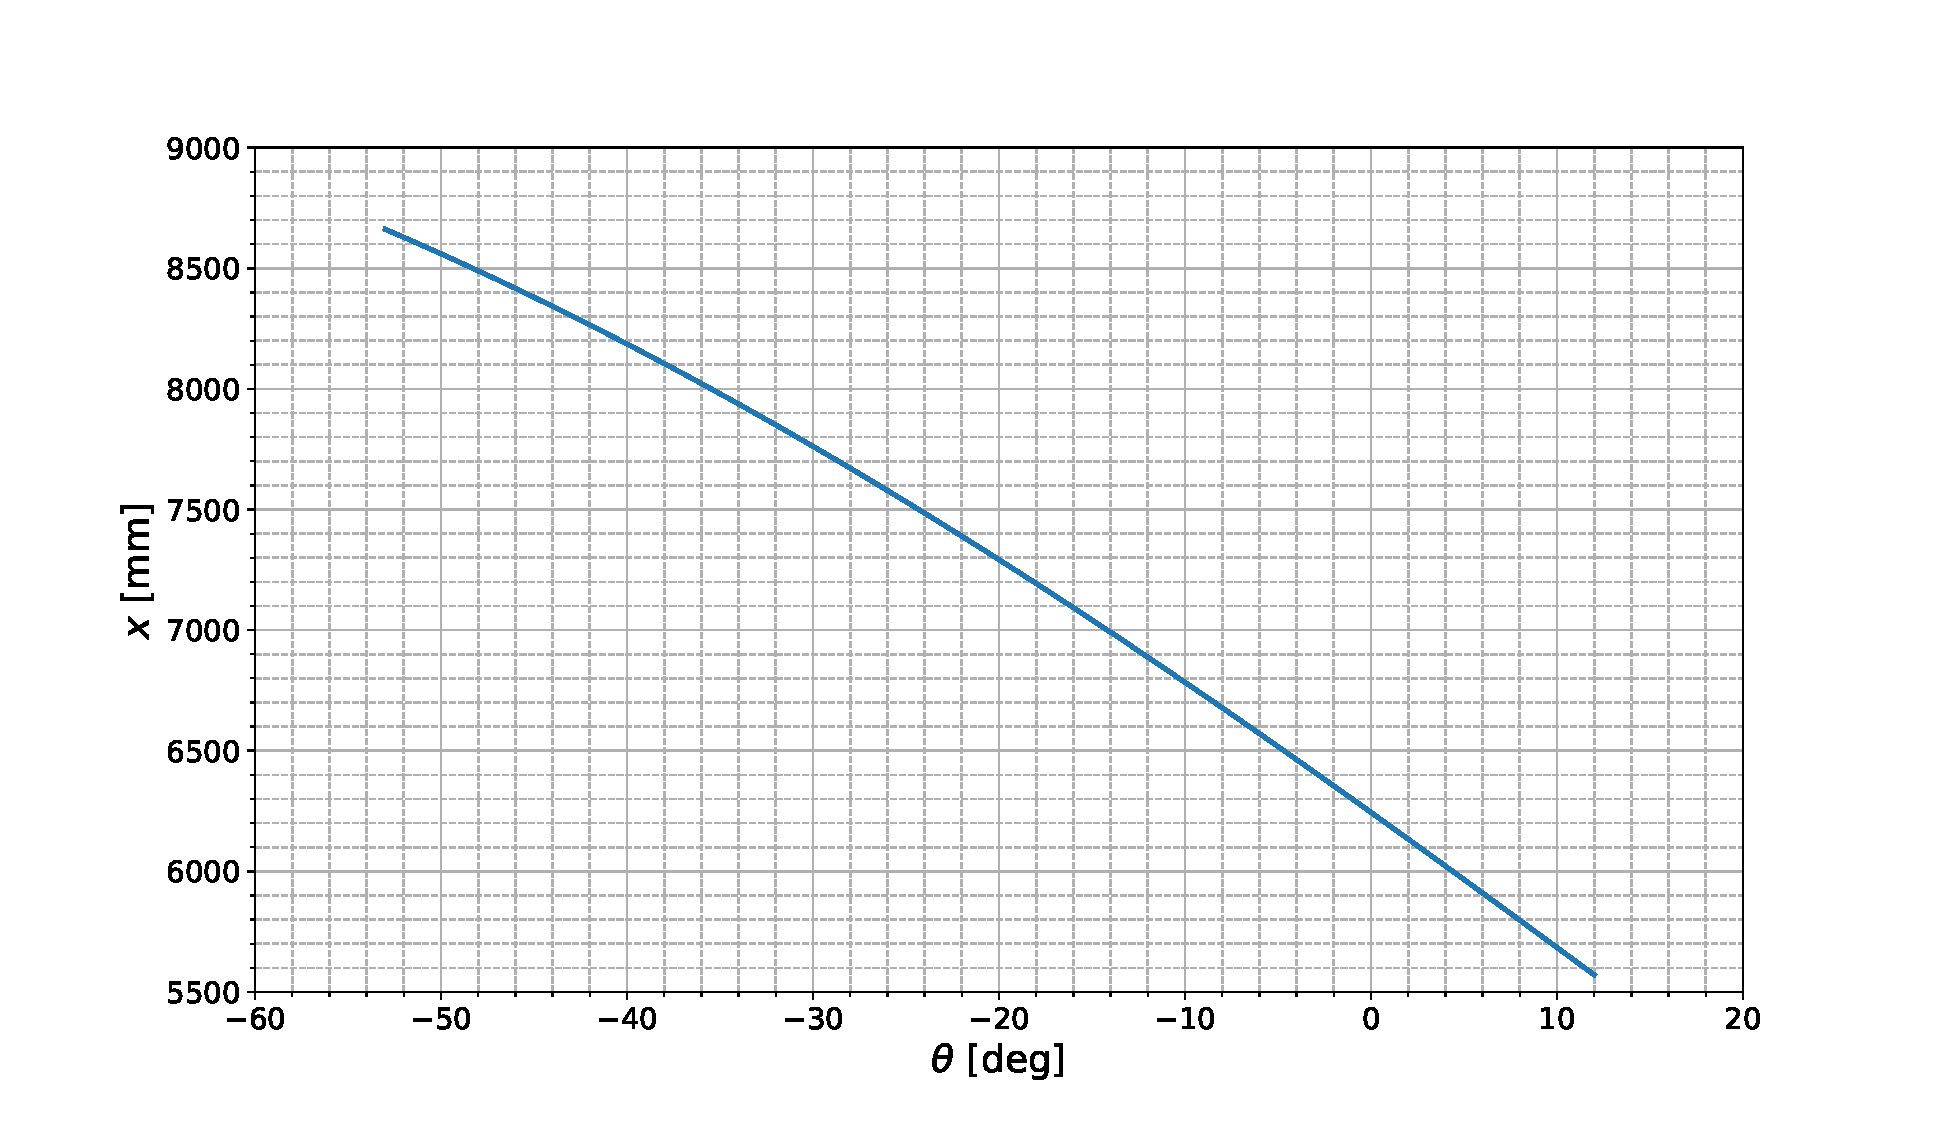
\includegraphics[width=0.75\linewidth]{x_theta}
%\end{figure}
%
%
%\begin{figure}[H]
%\centering
%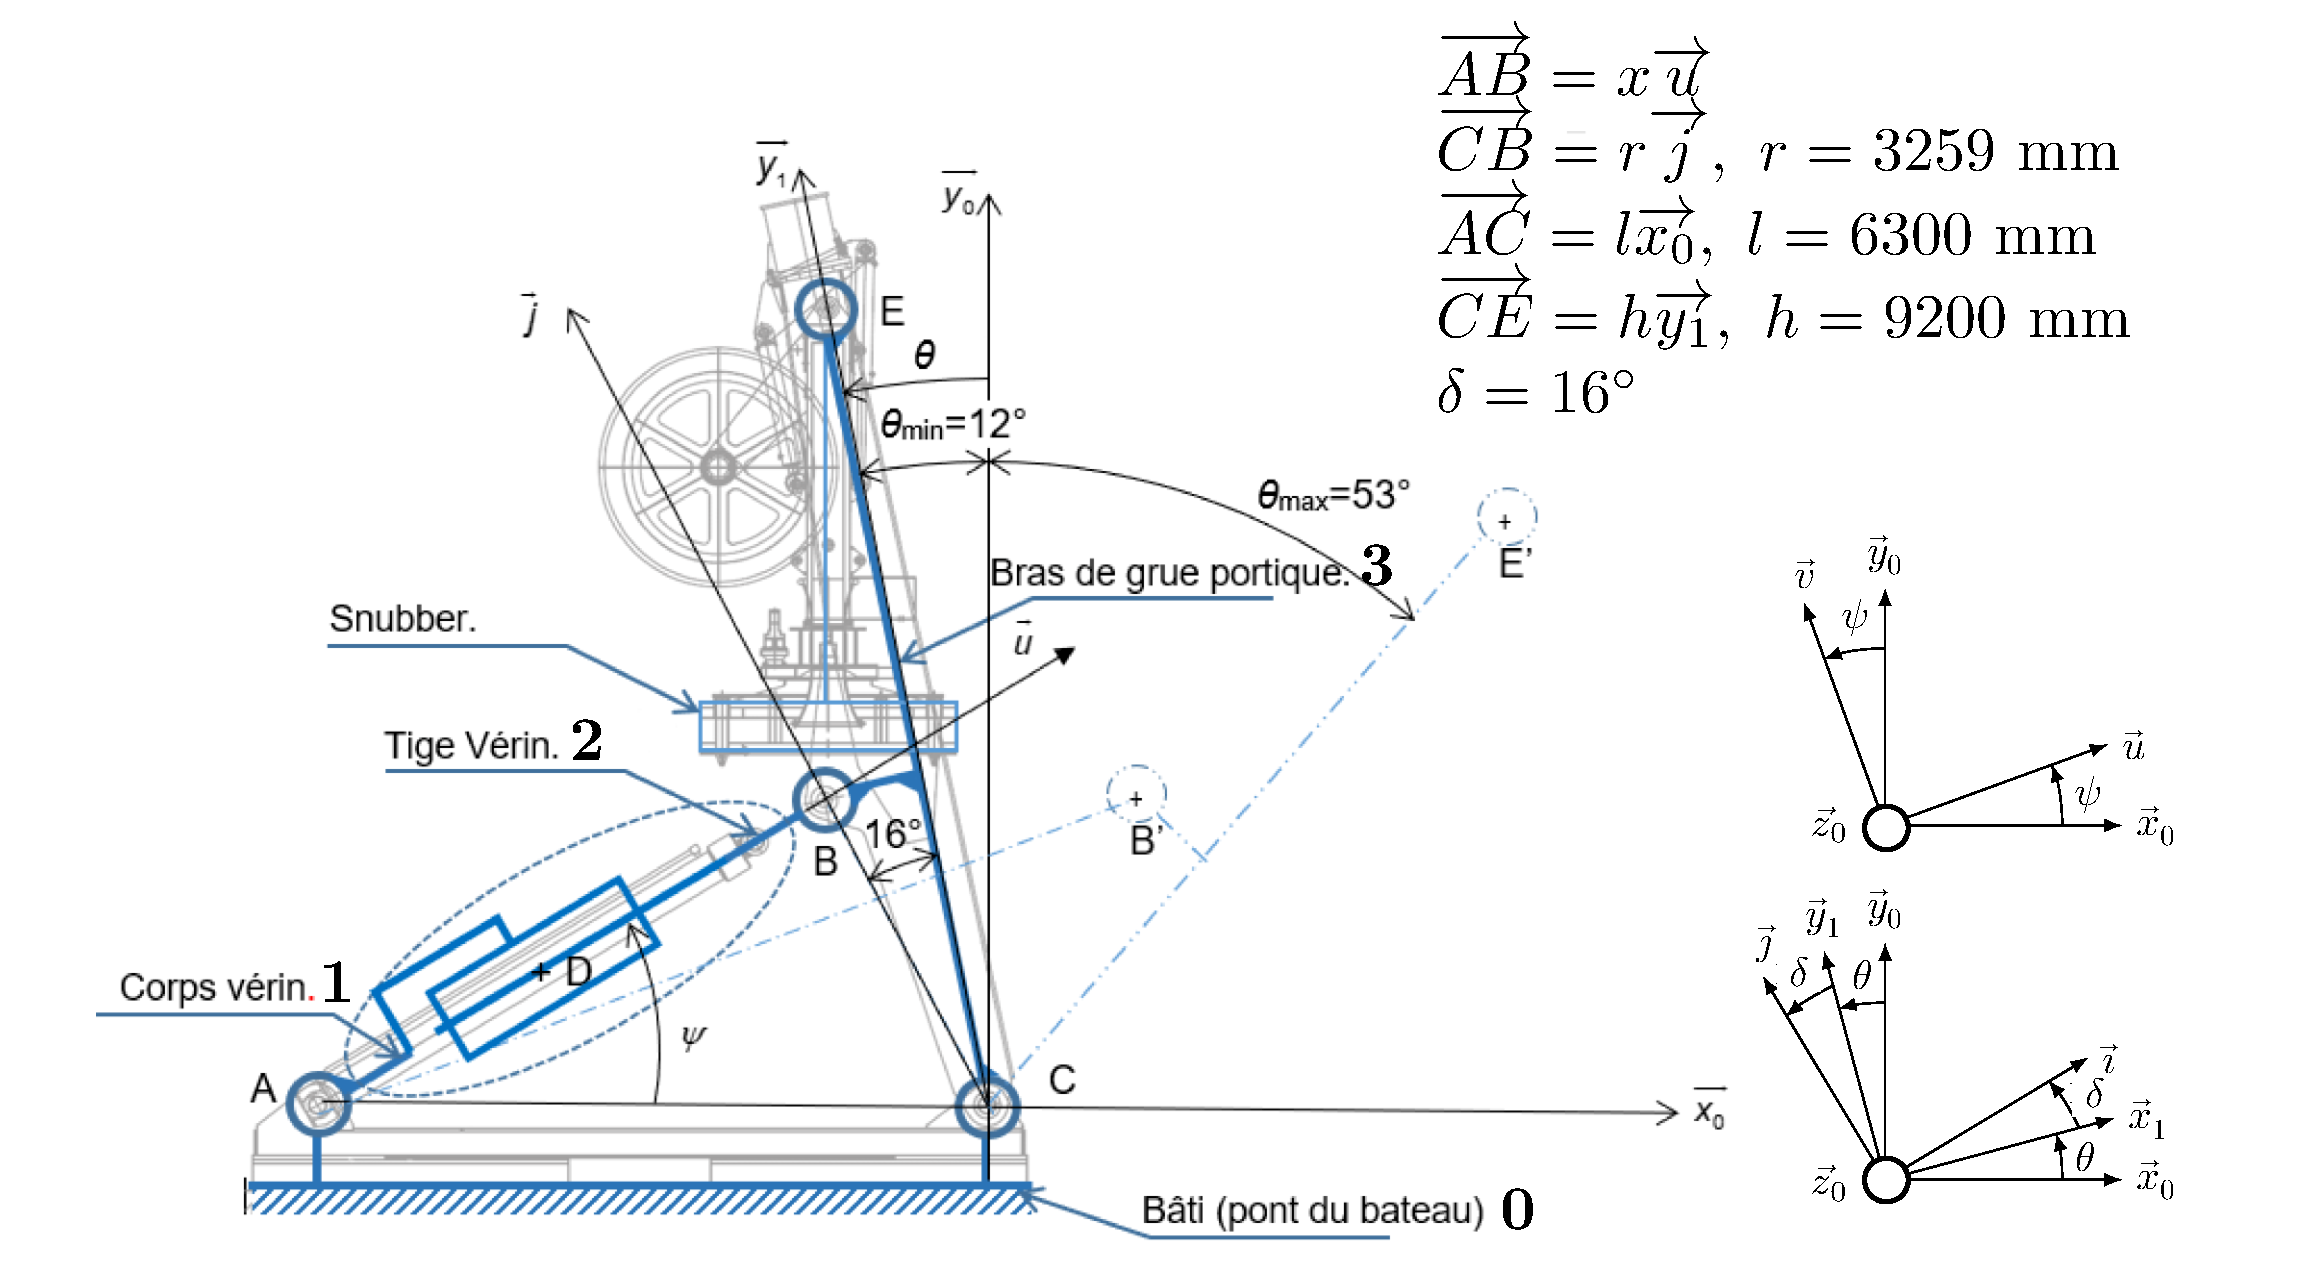
\includegraphics[width=0.75\linewidth]{SC}
%\end{figure}
%
%
%\end{corrige}
%\else
%\fi
%
%
%
%La simulation avec une analyse géométrique à l’aide du modèle multiphysique complet a permis d’obtenir la courbe donnée sur la \autoref{Fig7}.\\
%
%
%\question{À partir de la \autoref{Fig4} et du schéma cinématique \autoref{Fig6}, relier les composants du modèle de simulation
%multiphysique de la grue portique sur la Figure B du document réponse. Quel(s) ensemble(s) n’ont pas été
%modélisés ? Répondre entièrement à cette question sur le document réponse.}
%
%\ifprof
%\begin{corrige}
%%\textbf{Q5} 
%Les ensembles non modélisés sont la poulie de grue, le câble ombilical, le snubber et le ROV (leur poids sera appliqué au portique pour tenir compte de leur effet).
%
%\begin{figure}[H]
%\centering
%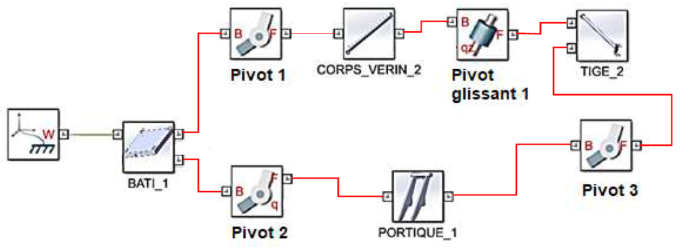
\includegraphics[width=0.65\linewidth]{Q5}
%\end{figure}
%
%
%\end{corrige}
%\else
%\fi
%
%
%\question{À partir de la courbe de simulation, déterminer la course du vérin notée $c$. Comparer le résultat à
%celui obtenu à la question 4}.
%
%\ifprof
%\begin{corrige}
%%\textbf{Q6}   
%Graphiquement, on lit : $c\approx 8655-5600=3065$ mm, ce qui correspond, aux erreurs de lecture pr\`es, \`a la course calculée par fermeture géométrique.\\
%
%
%\end{corrige}
%\else
%\fi
%
%
%\question{Déterminer l’expression de la résultante de l’effort de la tige du vérin sur le bras de la grue portique, noté $\overrightarrow F_{\text{tige}\to \text{bras}}$. Pour cela, justifier que $\overrightarrow F_{\text{tige}\to \text{bras}}=F_{\text{tige}\to \text{bras}}\overrightarrow u$. Déterminer ensuite $F_{\text{tige}\to \text{bras}}$ en fonction de $\theta$, $\psi$, des paramètres dimensionnels $h$ \textbf{(erreur de  notation $h=d$)}, $r$ et $\delta$ et des données associées aux actions mécaniques en précisant le ou les
%systèmes isolés et le ou les théorèmes employés.}
%
%\ifprof
%\begin{corrige}
%%\textbf{Q7}  
%Le syst\`eme de solides est une chaine fermée. On cherche l'effort de la tige du vérin \textbf 2 sur la bras \textbf 3. \\
%
%\textbf{1.} On isole \{\textbf 1;\textbf 2\} (le vérin), qui est soumis \`a deux glisseurs (deux liaisons rotule en 3d en $A$ et en $B$). L'effort de \textbf 3 sur \textbf 2 est donc colinéaires \`a $\overrightarrow{AB}$ donc \`a $\overrightarrow u$. Ainsi :
%
%$$\begin{Bmatrix}\mathcal T_{3\to2}\end{Bmatrix}=\begin{Bmatrix}F_{32}\overrightarrow u\\
%\overrightarrow 0 \end{Bmatrix}_B.$$
%
%
%
%\textbf{2.} On isole \textbf 3 soumis \`a :
%\begin{itemize}
%\item l'action mécanique transmissible par la liaison rotule entre \textbf 2 et \textbf 3 $\begin{Bmatrix}\mathcal T_{2\to3}\end{Bmatrix}=-\begin{Bmatrix}\mathcal T_{3\to2}\end{Bmatrix}=\begin{Bmatrix}F_{23}\overrightarrow u\\
%\overrightarrow 0
%\end{Bmatrix}_B$,
%\item l'action mécanique transmissible par la liaison rotule entre \textbf 0 et \textbf 3 $\begin{Bmatrix}\mathcal T_{0\to3}\end{Bmatrix} = \begin{Bmatrix} X_{03}\overrightarrow{x_0} +Y_{03}\overrightarrow{y_0}+Z_{03}\overrightarrow{z_0}   \\
%L_{03}\overrightarrow{x_0} +M_{03}\overrightarrow{y_0}   \end{Bmatrix}_C,$
%\item l'action du ROV sur \textbf 3 $\begin{Bmatrix}\mathcal T_{ROV \to3}\end{Bmatrix} = \begin{Bmatrix} -Mg\overrightarrow{y_0}\\ 
%\overrightarrow 0 \end{Bmatrix}_E$, 
% \end{itemize}
% 
% On applique le TMS en $C$ pour ne pas faire apparaitre les inconnues de liaison entre \textbf 0 et \textbf 3.
% \begin{eqnarray}
% \overrightarrow{CB}\wedge F_{23}\overrightarrow u+\overrightarrow{CE}\wedge -Mg\overrightarrow{y_0}&=&\overrightarrow 0,\nonumber \\
%r \overrightarrow{j}\wedge F_{23}\overrightarrow u+h\overrightarrow{y_1}\wedge -Mg\overrightarrow{y_0}&=&\overrightarrow 0,\nonumber \\ 
%- r F_{23} \cos(\delta+\theta-\psi)\overrightarrow{z_0} + hMg \sin\theta\overrightarrow{z_0}&=&\overrightarrow 0.\nonumber 
% \end{eqnarray}
% 
% On trouve :
%$$ \boxed{F_{23} = \dfrac{hMg \sin\theta}{r\cos(\delta+\theta-\psi)}.}$$
% 
% 
% 
%\textcolor{red}{Ci-dessous le tracé de l’effort $F_{23}$ en fonction de l’angle $\theta$ avec les signes corrigés (qui est un peu différente de la Figure 8 du sujet.}
% 
%\begin{figure}[H]
%\centering
%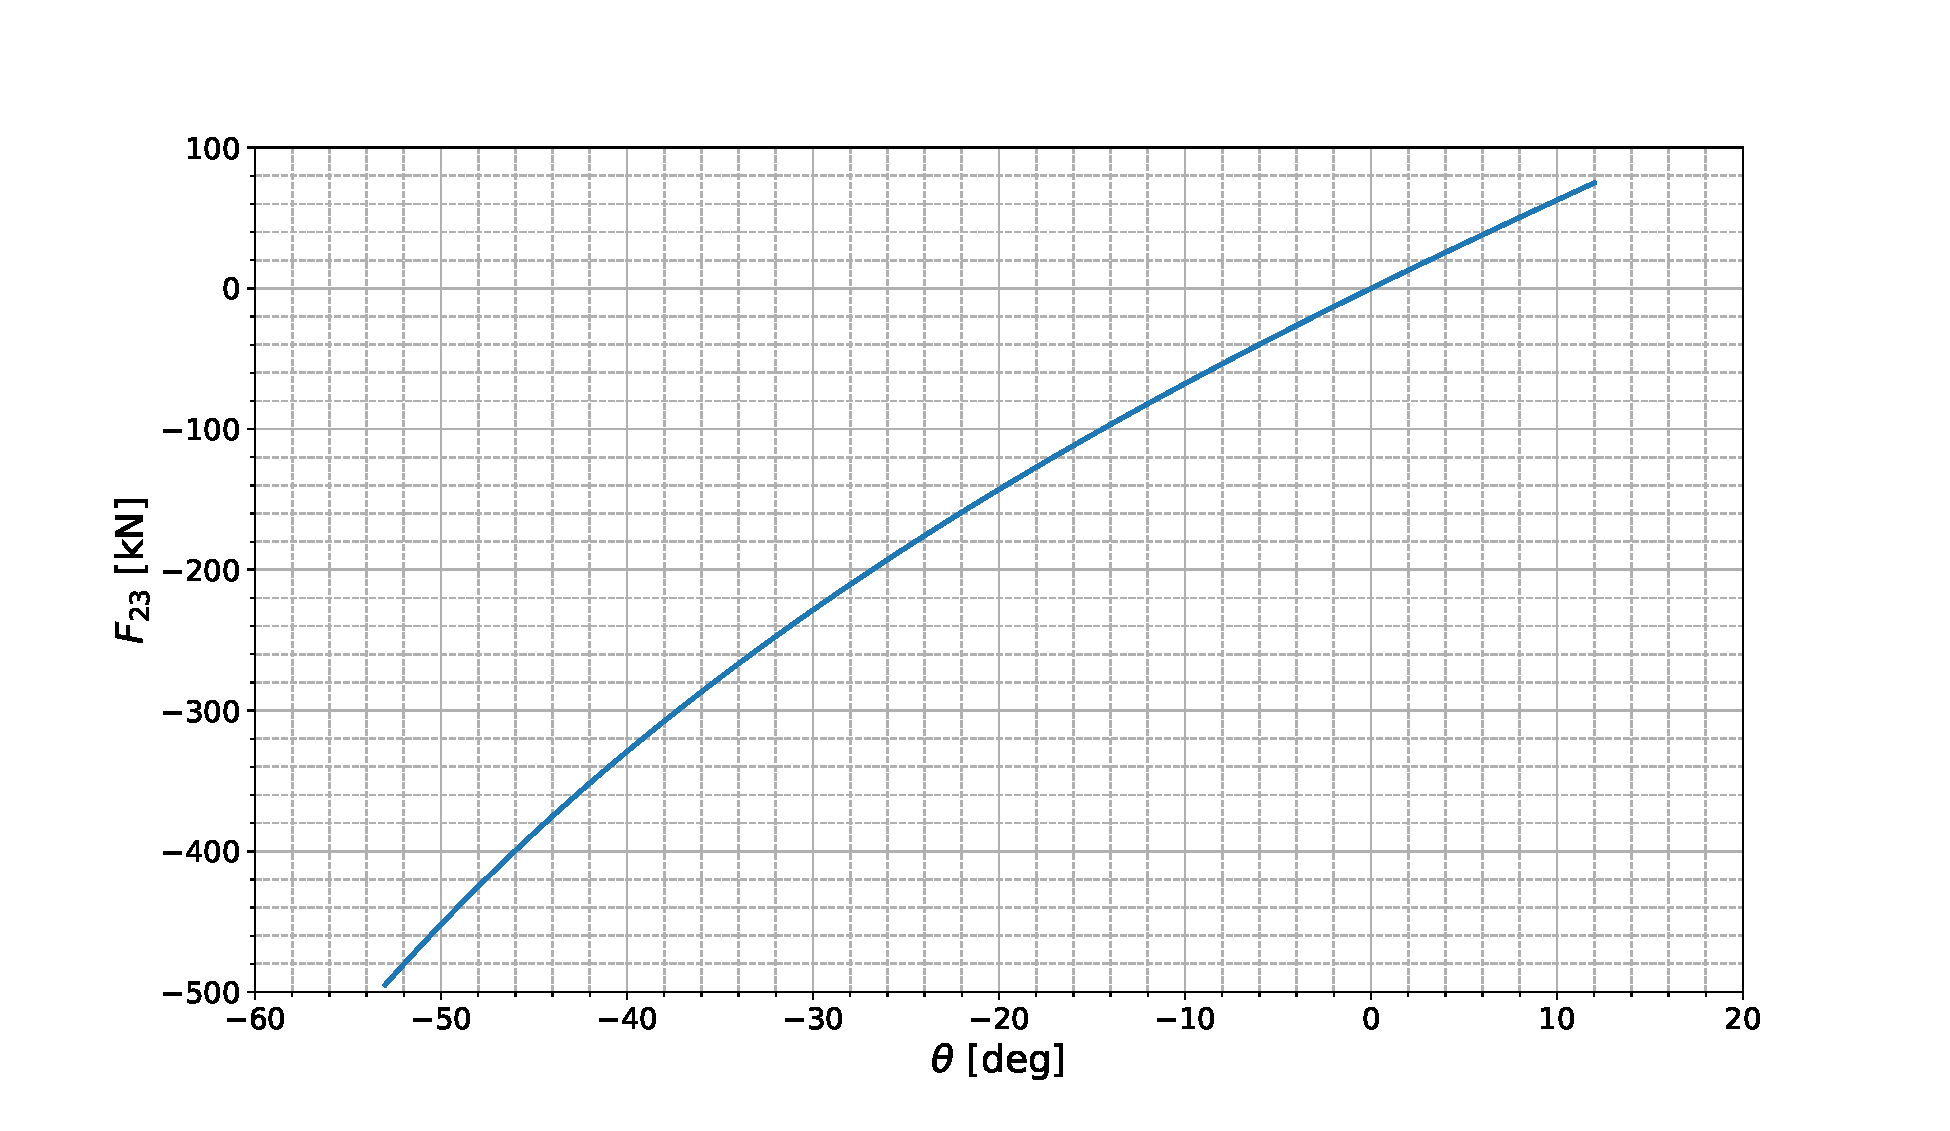
\includegraphics[width=0.75\linewidth]{F_theta}
%\end{figure}
%
%\end{corrige}
%\else
%\fi
%
%
%\ifprof
%\else
%
%Le résultat de ce calcul combiné à la loi entrée sortie $\psi = f(\theta)$ permettent d’obtenir un résultat identique à
%celui obtenu par simulation pour une étude statique dont la courbe résultat est donnée sur la \autoref{Fig8}. \\
%\textbf{Remarque} : la
%simulation prend en compte la majoration de la norme et les résultats donnés pour un seul vérin.\\
%
%
%\begin{figure}[H]
%\centering
%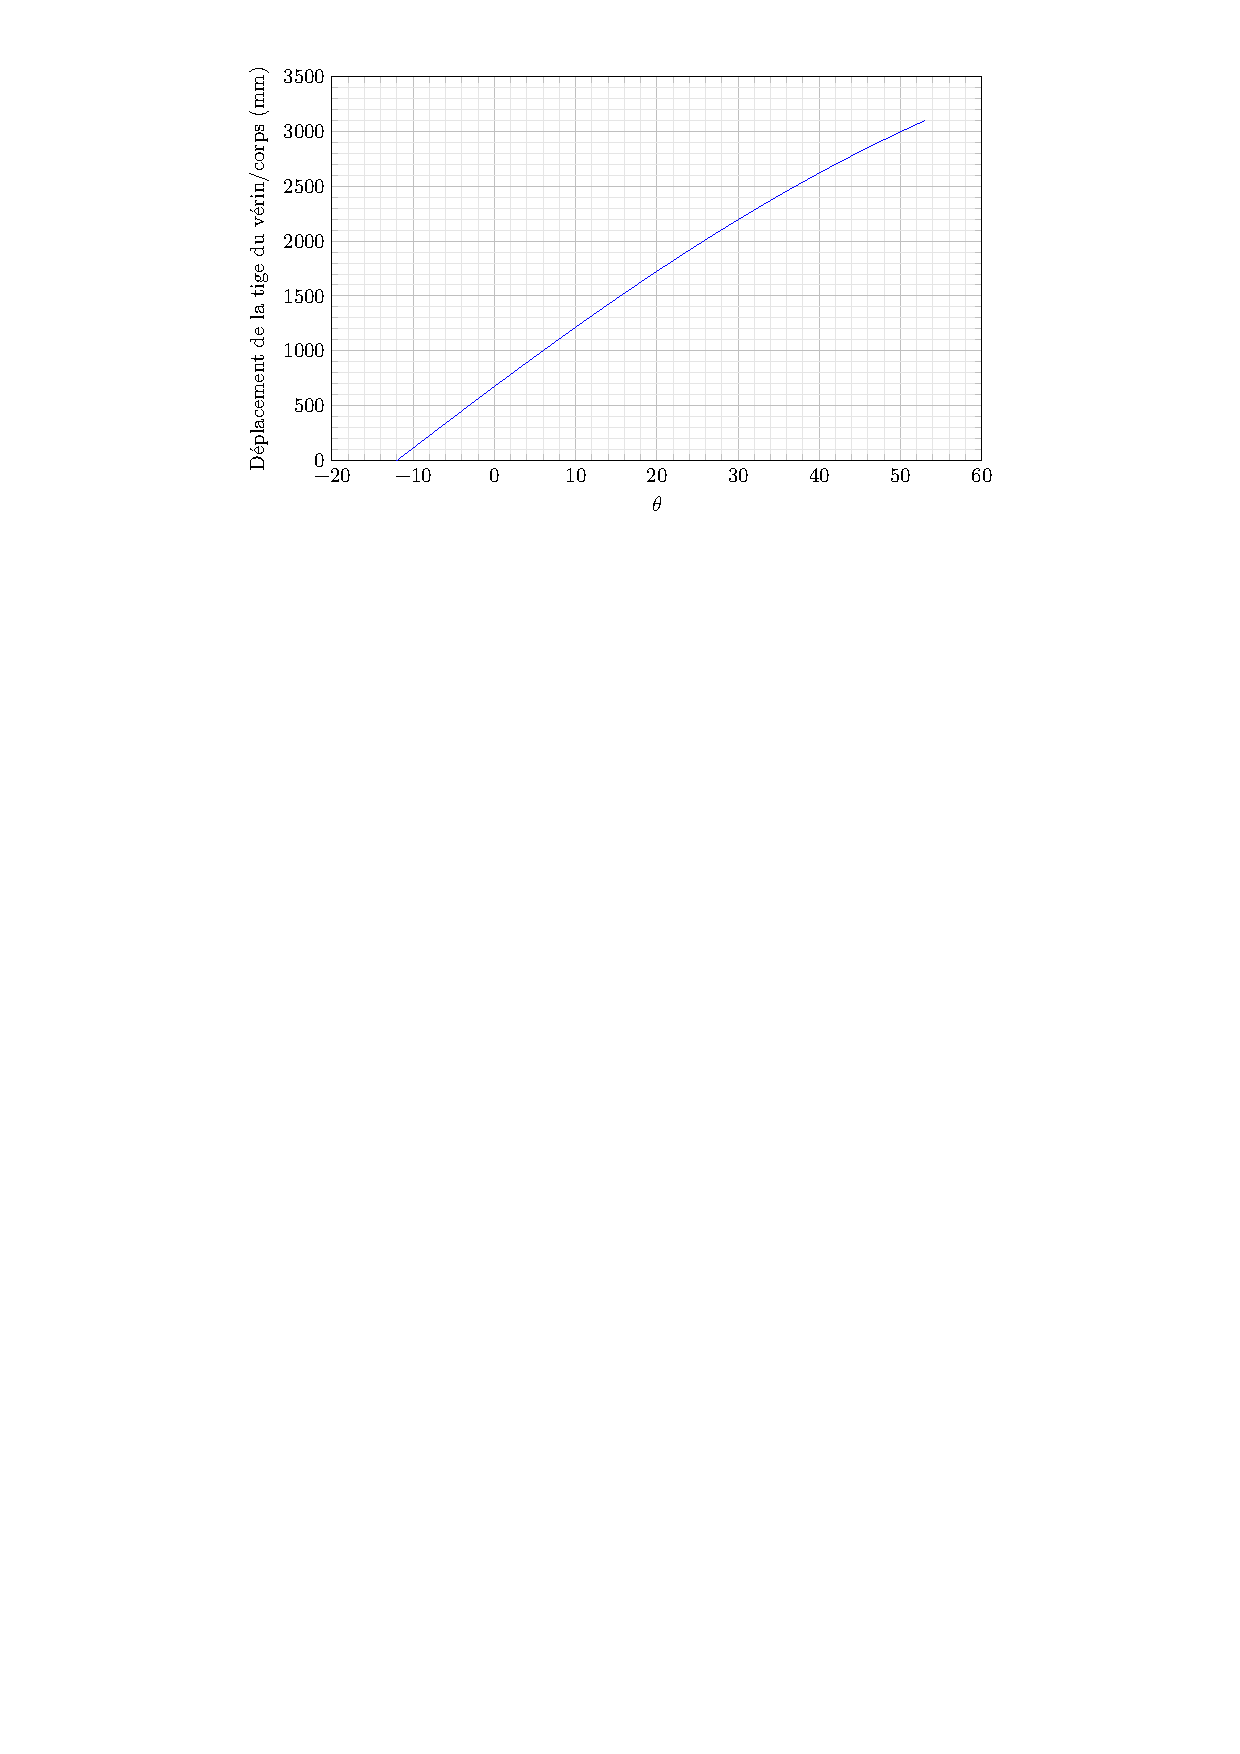
\includegraphics[width=0.7\linewidth]{Fig7}
%\caption{Déplacement de la tige du vérin en fonction de $\theta$}
%\label{Fig7}
%\end{figure}
%
%\begin{figure}[H]
%\centering
%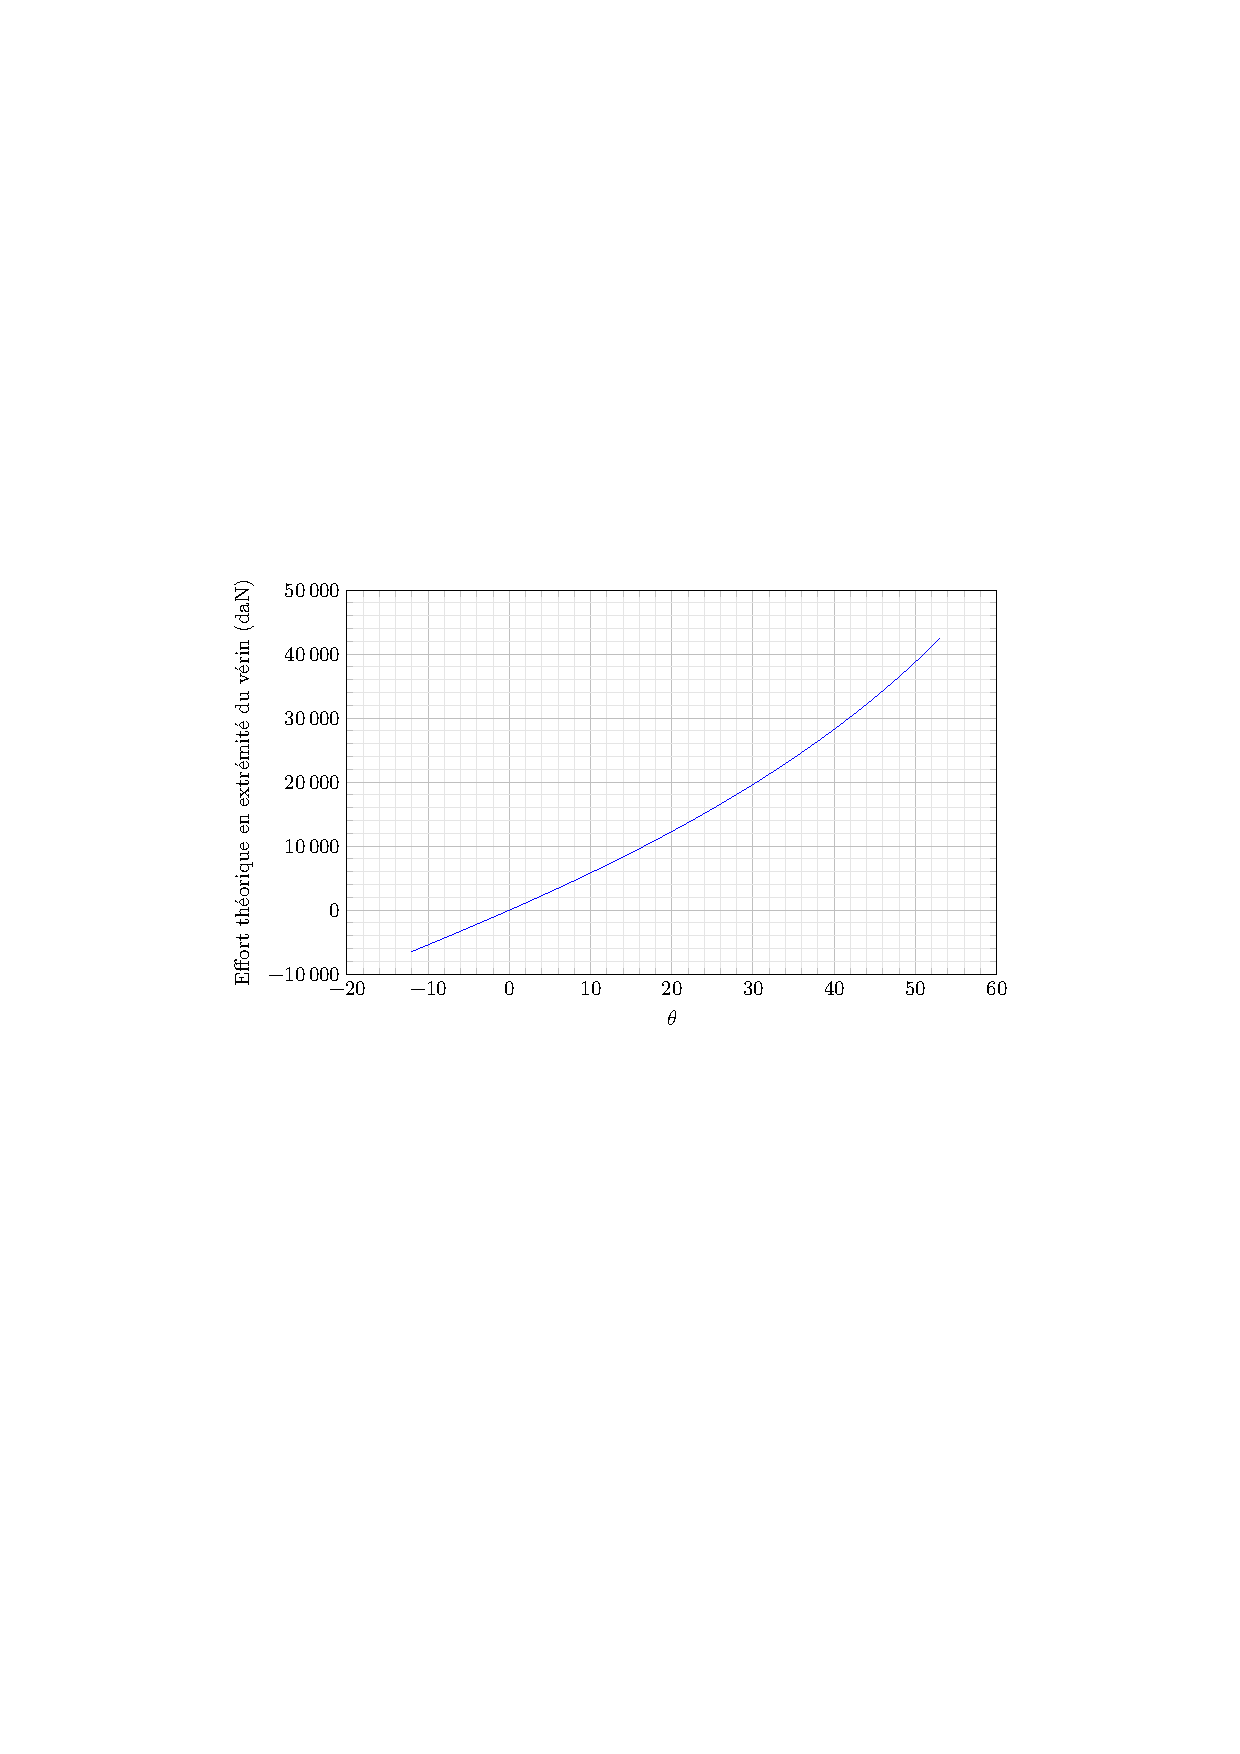
\includegraphics[width=0.7\linewidth]{Fig8}
%\caption{Effort à l’extrémité de la tige du vérin en fonction de $\theta$}
%\label{Fig8}
%\end{figure}
%
%
%Le vérin utilisé a les caractéristiques suivantes :
%\begin{itemize}
%\item diamètre de la tige $d = 180$ mm ;
%\item diamètre du piston $D = 250$ mm ;
%\item course maximale $c_{\text{max}} = 3800$ mm ;
%\item le port A permet la sortie de la tige, le port B la rentrée ;
%\item le circuit hydraulique peut délivrer une pression maximale de 200 bar.
%\end{itemize}
%
%
%\begin{figure}[H]
%\centering
%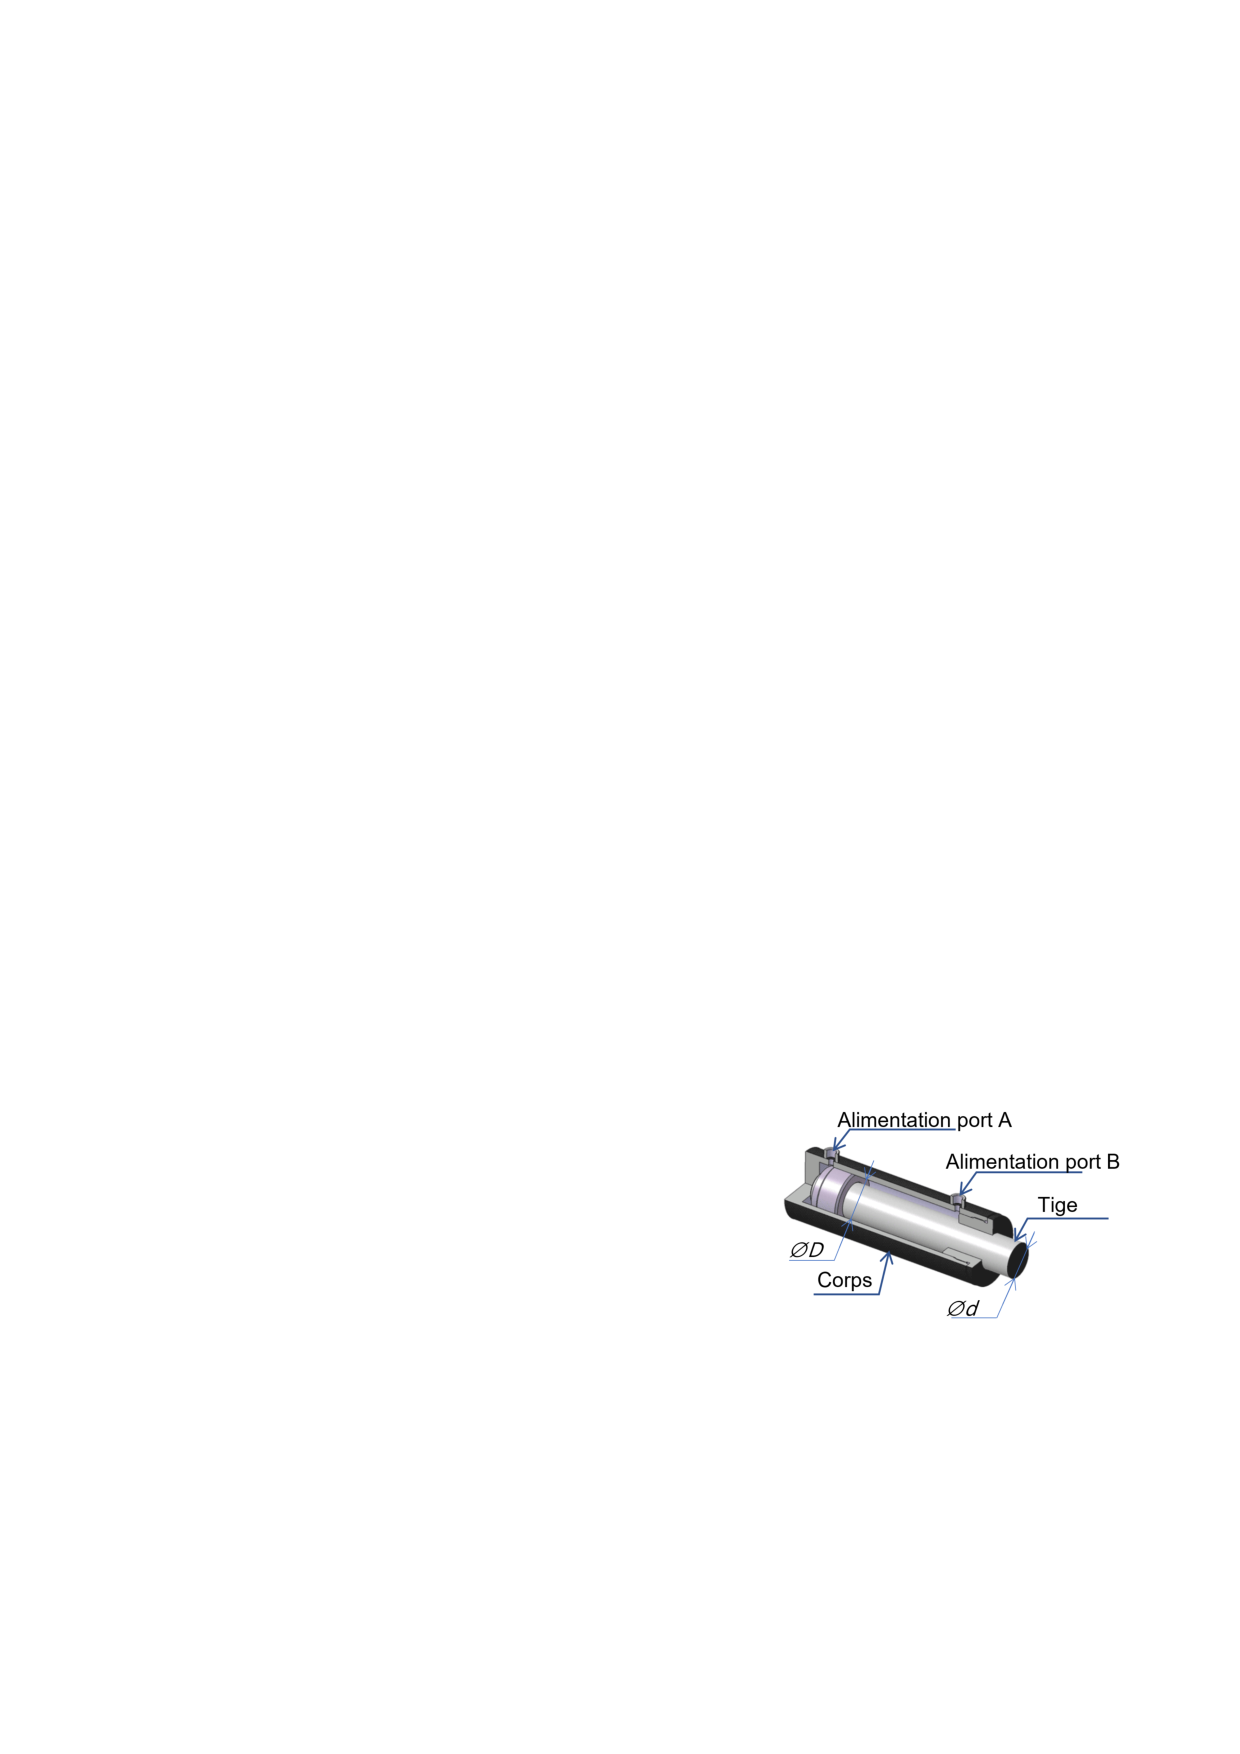
\includegraphics[width=0.35\linewidth]{Fig9}
%\caption{ Vue en quart de coupe du vérin}
%\label{Fig9}
%\end{figure}
%
%\fi
%\question{Déterminer la pression d’alimentation théorique maximale du vérin nécessaire pour assurer le maintien
%du portique dans la position la plus défavorable. Est-elle compatible avec le circuit hydraulique ?}
%
%\ifprof
%\begin{corrige}
% %\textbf{Q8}  
%  Pour un effort « en poussant » (soit dans le sens de la sortie de la tige), la pression d’huile nécessaire est :
%$$p=\dfrac{|F_{23}|}{S_{\text{sortie}}} =\dfrac{|F_{23}|}{\pi D^2/4}.$$
% 
%De même pour un effort « de retenue » (soit dans le sens de la rentrée de la tige) :
% $$p=\dfrac{|F_{23}|}{S_{\text{sortie}}} =\dfrac{|F_{23}|}{\pi (D^2-d^2)/4}.$$
% 
%Selon la Figure 8 du sujet, l’effort (en valeur absolue) est maximal pour $\theta=53^\circ$ ($\theta=-53^\circ$), soit en rentrée de tige avec $|F_{23max}| \approx 425$ kN, soit $p_{\text{max}}=180$ bar.\\
% 
%%On peut vérifier le dimensionnement en sortie de tige, on a alors $|F_{23max} |\approx 80$ kN, soit $p_{\text{max}}=16,3$ bar.\\
% 
%\end{corrige}
%\else
%\fi
%
%\question{Conclure sur le choix du vérin à partir des résultats des questions précédentes.}
%
%\ifprof
%\begin{corrige}
%% \textbf{Q9}   
% La pression maximale est atteinte dans le premier cas étudié ($\theta=-53^\circ$) et elle est inférieure à la pression maximale que peut délivrer le circuit hydraulique (attention, les effets dynamiques sont négligés ici). D’autre part, la course nécessaire (3100 mm) est inférieure à la course maximale du vérin (3800 mm). Donc le choix du vérin est validé suivant deux critères, géométrique et statique. \\
% \end{corrige}
% \else
% \fi
% 
%
%L’étude précédente a été faite dans la phase de transfert du ROV, celui-ci étant accroché au snubber. Une
%démarche similaire de dimensionnement du vérin a montré que le résultat de la question 8 reste valable lors de
%la phase de descente, le ROV étant accroché au câble.
%

\section*{Étude du système de compensation de houle PHC (Passiv Heave
Compensator)}
\begin{obj}
Dimensionner un système passif de compensation de la houle et tester sa conformité aux exigences du
cahier des charges.
\end{obj}

\ifprof
\else
Pour compenser les effets de la houle, une solution hydropneumatique est alors envisagée. Ce système est un
compensateur de houle passif noté PHC (\autoref{Fig10}).\\


\begin{figure}[H]
\centering
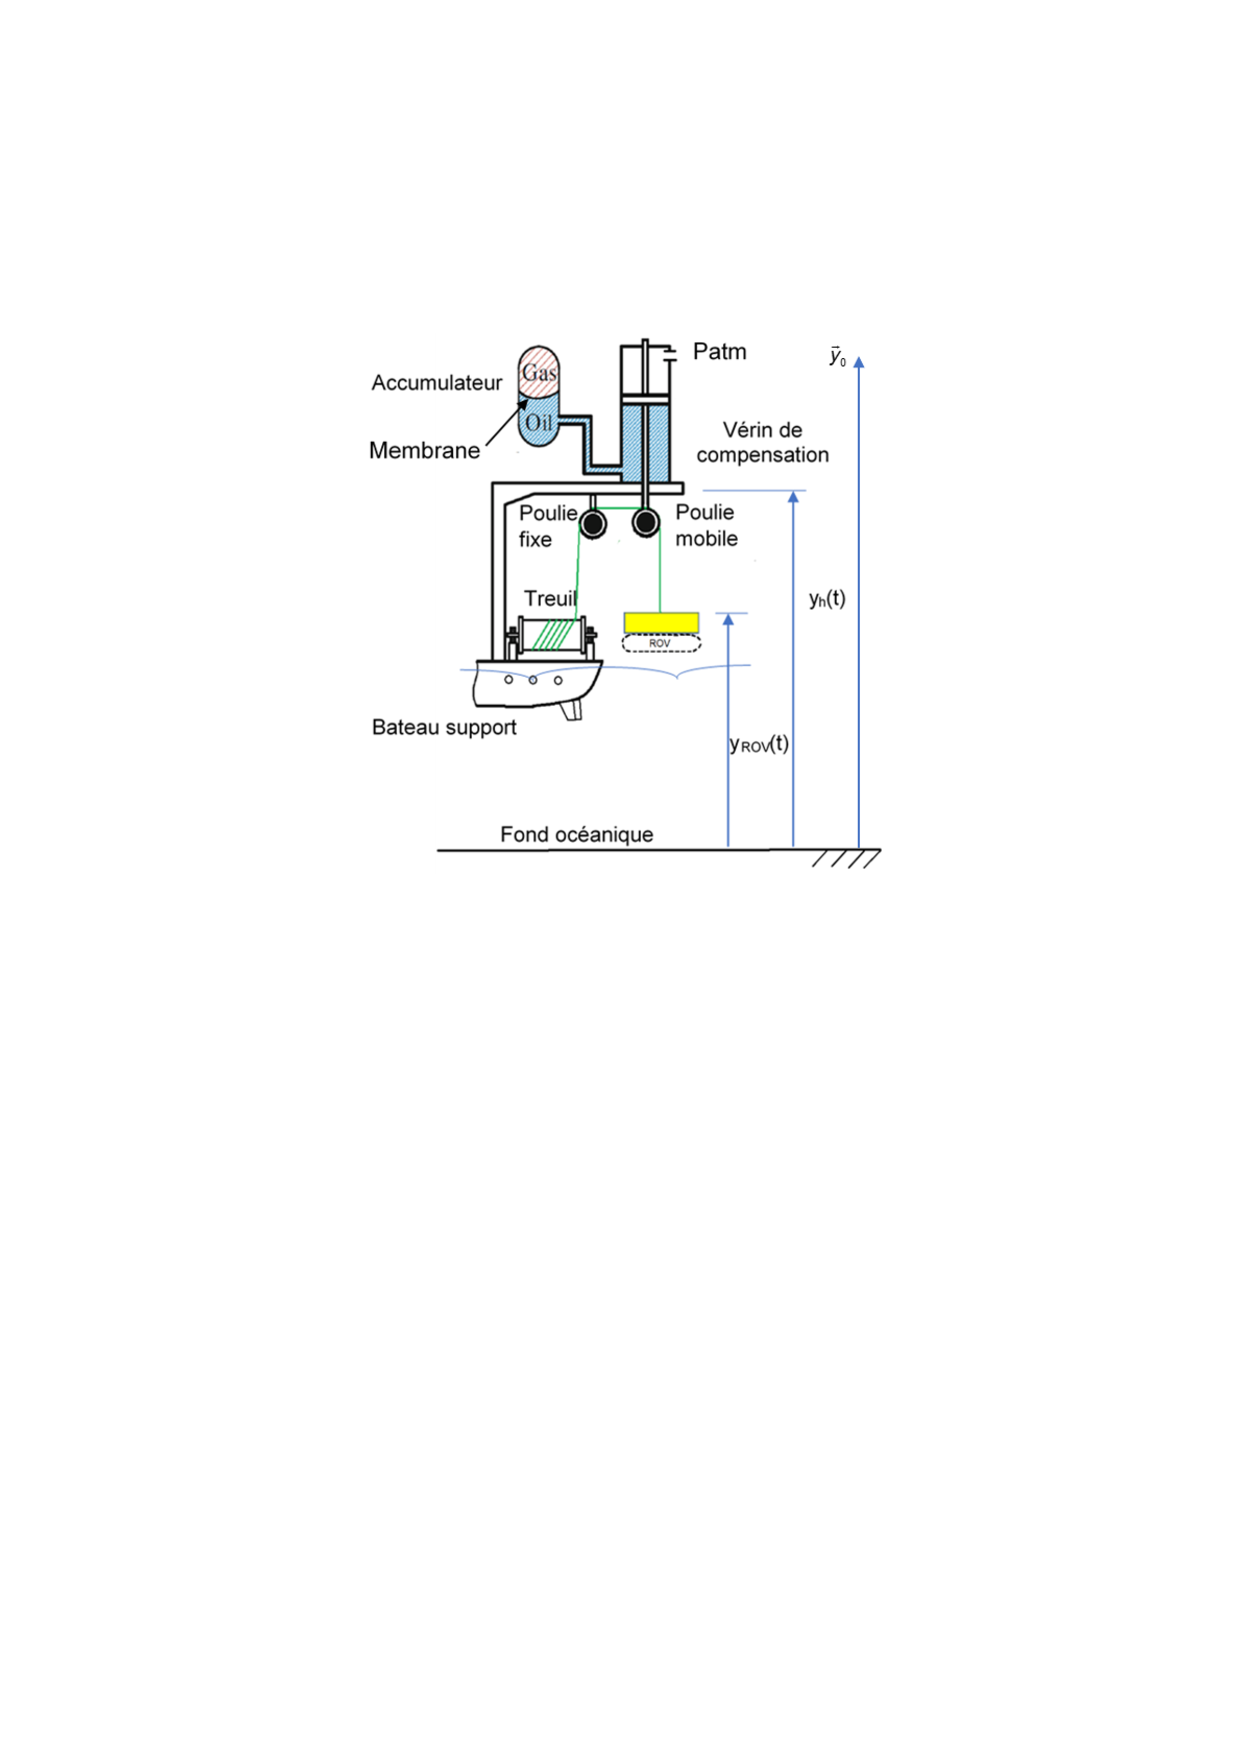
\includegraphics[width=0.65\linewidth]{Fig10}
\caption{ Schéma d’implantation du PHV (non à l’échelle)}
\label{Fig10}
\end{figure}




%\textbf{Notations et hypothèses} 
%\begin{itemize}
%\item le déplacement du bateau est noté $y_h(t)$ ;
%\item le déplacement du ROV hors de l’eau est noté $y_{\text{ROV}}(t)$ ;
%\item le vérin de compensation hydraulique a des surfaces actives de part et d’autre du piston égales et notées $A$ en $\text{m}^2$ ;
%\item le vérin de compensation hydraulique a une force d’amortissement linéaire de coefficient d’amortissement
%visqueux $c = 100 \ \text N\cdot \text s\cdot \text m^{-1}$ ;
%\item la masse suspendue du ROV et du système d’accroche est considérée constante $M = 26$ t (majoration de 100 \%) ;
%\item les masses des autres pièces sont négligeables ;
%\item le treuil est considéré bloqué pendant la phase étudiée ;
%\item l’huile hydraulique (oil) est compressible avec un module de masse $K$, ce qui signifie que la variation de
%pression du vérin affecte le volume d’huile $V_E$ ;
%\item l’ensemble du bateau support est considéré rigide ;
%\item la transformée de Laplace de la fonction $y_i(t)$ est notée $Y_i(p)$ ;
%\item les transformées de Laplace des fonctions $\Delta p_E(t)$ et $\Delta p_G(t)$ sont notées respectivement $\Delta P_E(p)$ et $\Delta P_G(p)$.
%\end{itemize}
%\noindent Les grandeurs statiques à l’équilibre sont :
%\begin{itemize}
%\item le volume de gaz dans l’accumulateur $V_{G0}$ ;
%\item la pression de gaz dans l’accumulateur $P_{G0}$ ;
%\item la pression d’huile dans la chambre active du vérin $P_{E0}$.
%\end{itemize}
%\noindent Les variables dynamiques sont :
%\begin{itemize}
%\item la pression du gaz dans l’accumulateur $p_G(t)$ ;
%\item la pression d’huile dans la chambre active du vérin $p_E(t)$.
%\end{itemize}
%\noindent Les paramètres hydrauliques sont :
%\begin{itemize}
%\item le coefficient polytropique de la compression du gaz $r = 1,33$ ;
%\item la conductivité hydraulique entre le vérin et l’accumulateur $C_{qR}$ .
%\end{itemize}


Les petites variations de pression $\Delta p_E(t)$ et $\Delta p_G(t)$ autour du point d’équilibre peuvent être
définies par $\Delta p_E(t) = p_E(t) - P_{E0}$ et $\Delta p_G(t) = p_G(t) -P_{G0}$.
Une étude de mécanique des fluides a permis d’obtenir les relations (1) et (2).

$
\begin{array}{ccc}
\dfrac{\text d\Delta p_E(t)}{\text dt} &=& \dfrac{K}{V_E} S\left( \dfrac{\text d y_h(t)}{\text dt}-\dfrac{\text d y_{\text{ROV}}(t)}{\text dt}\right) \\ 
&& +\dfrac{K}{V_E} C_{qR}\left(\Delta p_G(t)-\Delta p_E(t)\right) \; (1)
\end{array}$

$\dfrac{\text d\Delta p_G(t)}{\text dt}=\dfrac{rP_{G0}C_{qR}}{V_{G0}}\left(\Delta p_E(t)-\Delta p_G(t)\right)  \; (2)$.


\fi

%\question{Faire l’inventaire des actions mécaniques extérieures qui s’exercent sur le système matériel défini par $\Sigma  =$ \{ROV + snubber + Piston vérin + Poulie mobile\}. Écrire la condition d’équilibre du système matériel $\Sigma$ en
%donnant l’expression de $P_{E0}$ en fonction de $M$, $g$, $P_{\text{atm}}$ et $A$. On fera l’hypothèse que le câble entre les poulies fixe et mobile reste horizontal.}
%\ifprof
%\begin{corrige}
% 
%% \textbf{Q10}   
%On isole l'ensemble $\Sigma$. On dresse un bilan des AM extérieures :
% \begin{itemize}
% \item action de pesanteur $\to$ ROV ($-Mg\overrightarrow{y_0}$);
% \item action mécanique du \`a la différence de pression sur les 2 surfaces actives du vérin ($A(P_{E0}-P_{\text{atm}})\overrightarrow{y_0}$) ;
% \item tension dans le câble ou action du treuil sur le câble (effort horizontal) ;
% \item action mécanique transmissible par la liaison entre le piston et le corps (effort horizontal).
% \end{itemize}
% 
% On applique le TRS en projection suivant $\overrightarrow{y_0}$. On obtient :
% $$\boxed{-Mg + A(P_{E0}-P_{\text{atm}})=0.}$$
% 
% 
%\end{corrige}
%\else
%\fi
\ifprof
\else
À l'équilibre, le principe fondamental de la statique se traduit par $-Mg + S(P_{E0}-P_{\text{atm}})=0$.

%\question{L’équilibre de la membrane permet d’obtenir l’égalité $P_{E0} = P_{G0} = 180$ bar. En déduire la valeur de $A$.}
%\ifprof
%\begin{corrige}
%
% %\textbf{Q11}   
% Si on néglige $P_{\text{atm}}$ devant la pression $P_{E0}$, on obtient :
% $$\boxed{S=\dfrac{Mg}{P_{E0}}=\dfrac{Mg}{P_{G0}}\approx 14249 \  \text{mm}^2.}$$
%  
%\end{corrige}
%\else
%\fi
%

Le théorème de la résultante dynamique appliqué à $\Sigma$ se traduit par 
%$\alpha \dfrac{\text d^2y_{\text{ROV}}(t)}{\text d t^2}+\beta \left(\dfrac{\text dy_{\text{ROV}}(t)}{\text dt}-\dfrac{\text d y_h(t)}{\text dt}\right)&=&\gamma \Delta p_E(t).$
$ S\Delta p_E(t)=M\ddot y_{\text{ROV}}(t)+c(\dot y_{\text{ROV}}(t)-\dot y_h(t) ) $ (3).
% avec $\gamma =S$, $\alpha =M$ et $\beta = c$.\\



%\question{Déterminer l’équation, notée (3), issue du théorème de la résultante dynamique appliqué à $\Sigma$ en projection sur $\overrightarrow{y_0}$ sous la forme :}
%
%\begin{eqnarray}
%\alpha \dfrac{\text d^2y_{\text{ROV}}(t)}{\text d t^2}+\beta \left(\dfrac{\text dy_{\text{ROV}}(t)}{\text dt}-\dfrac{\text d y_h(t)}{\text dt}\right)&=&\gamma \Delta p_E(t).
%\end{eqnarray}
%
%\textit{Exprimer $\alpha$, $\beta$ et $\gamma$ en fonction de $A$, $M$ et $c$.}\\
%
%
%\ifprof
%\begin{corrige}
% %\textbf{Q12}   
% On isole l'ensemble $\Sigma$. On dresse un bilan des AM extérieures :
% 
%  \begin{itemize}
% \item action de pesanteur $\to$ ROV ($-Mg\overrightarrow{y_0}$);
% \item action mécanique du \`a la différence de pression sur les 2 surfaces actives du vérin ($A(p_{E}(t)-P_{\text{atm}})\overrightarrow{y_0}$) ;
% \item tension dans le câble (effort horizontal) ;
% \item tension dans le câble ou action du treuil sur le câble (effort horizontal) ;
% \item action mécanique transmissible par la liaison entre le piston et le corps (effort horizontal) ;
%   \item force d'amortissement linéaire dans le vérin $-c(\dot y_{\text{ROV}}(t)-\dot y_h(t) )\overrightarrow{y_0}$.
% \end{itemize}
% 
%Le frottement visqueux dans le vérin à tendance à ralentir le mouvement de la tige du vérin et il est proportionnel à la vitesse de translation de la tige du vérin par rapport au bateau (mouvement de translation, cette vitesse peut être écrite en tout point) : 
%$\overrightarrow V_{M,\text{tige⁄bateau}}=\overrightarrow V_{M,\text{tige}⁄0}-\overrightarrow V_{M,\text{bateau}⁄0}=(\dot y_{\text{ROV}}(t)-\dot y_h(t) )\overrightarrow{y_0}$.\\
%
%
%De plus, l'accélération du système isolé est $\Gamma_{M,\Sigma ⁄0}=\ddot y_{\text{ROV}}(t)$.\\
%
%
% On applique le principe fondamentale de la dynamique au syst\`eme $\Sigma$ en projection suivant $\overrightarrow{y_0}$. On obtient :
% $$-Mg + S(P_{E0}+\Delta p_E(t)-P_{\text{atm}})-c(\dot y_{\text{ROV}}(t)-\dot y_h(t) )=M\ddot y_{\text{ROV}}(t).$$
% 
% En utilisant la condition d'équilibre  ${-Mg + S(P_{E0}-P_{\text{atm}})=0}$, on obtient :
% 
%  
% $$\boxed{ S\Delta p_E(t)=M\ddot y_{\text{ROV}}(t)+c(\dot y_{\text{ROV}}(t)-\dot y_h(t) ),}$$
% avec $\gamma =S$, $\alpha =M$ et $\beta = c$.\\
% 
%\end{corrige}
%\else
%\fi
%


L’hypothèse du fluide incompressible se traduit par $\dfrac{\text d\Delta p_E(t)}{\text dt}= 0$.
\fi

\question{Réécrire l’équation (1) en tenant compte de cette hypothèse. Après avoir appliqué les transformées de Laplace aux équations (1) et (2) et en considérant les conditions initiales nulles aux équations précédentes, déterminer l’équation, notée (3), sous la forme :}
%\begin{eqnarray}
$\Delta P_E(p) = K_1(1+\tau_1 p)(Y_h(p)-Y_{\text{ROV}}(p))$ (4).
%\end{eqnarray}
\textit{Exprimer $K_1$ et $\tau_1$ en fonction de $A$, $V_{G0}$, $r$, $C_{qR}$ et $P_{G0}$.}
\ifprof
\begin{corrige}
% \textbf{Q13}   
On écrit les équations (1) et (2) dans le domaine de Laplace en tenant compte de l'hypothèse de fluide incompressible :
 \begin{eqnarray}
{Sp}\left( Y_h(p)-  Y_{\text{ROV}}(p)\right)+C_{qR}\left(\Delta P_G(p)-\Delta P_E(p)\right) &=&0, \\
\dfrac{rP_{G0}C_{qR}}{V_{G0}}\left(\Delta P_E(p)-\Delta P_G(p)\right) &=&p \Delta P_G(t).
\end{eqnarray}

L'équation (2) donne :
 \begin{eqnarray}
\Delta P_G(t)\left(p+\dfrac{rP_{G0}C_{qR}}{V_{G0}}\right)&=&\dfrac{rP_{G0}C_{qR}}{V_{G0}}\Delta P_E(p), \nonumber \\
\Delta P_G(t)&=&\dfrac{rP_{G0}C_{qR}}{pV_{G0}+{rP_{G0}C_{qR}}}\Delta P_E(p).\nonumber
\end{eqnarray}

En remplaçant dans (1), on obtient : 

 \begin{eqnarray}
{Sp}\left( Y_h(p)-  Y_{\text{ROV}}(p)\right)+C_{qR}\left(\dfrac{rP_{G0}C_{qR}}{pV_{G0}+{rP_{G0}C_{qR}}}\Delta P_E(p)-\Delta P_E(p)\right) &=&0, \nonumber
\end{eqnarray}
 \begin{eqnarray}
{Sp}\left( Y_h(p)-  Y_{\text{ROV}}(p)\right)&=&C_{qR}\left(1-\dfrac{rP_{G0}C_{qR}}{pV_{G0}+{rP_{G0}C_{qR}}}\right) \Delta P_E(p), \nonumber
\end{eqnarray}

 \begin{eqnarray}
\Delta P_E(p)&=&\dfrac{Sp}{C_{qR}}\dfrac{pV_{G0}+{rP_{G0}C_{qR}}}{pV_{G0} }\left( Y_h(p)-  Y_{\text{ROV}}(p)\right), \nonumber
\end{eqnarray}


 \begin{eqnarray}
\Delta P_E(p)&=&\dfrac{S}{C_{qR}}\dfrac{{rP_{G0}C_{qR}}}{V_{G0} }\left(\dfrac{V_{G0}}{{rP_{G0}C_{qR}} }p+1\right)\left( Y_h(p)-  Y_{\text{ROV}}(p)\right). \nonumber
\end{eqnarray}

Enfin, on obtient :
\begin{eqnarray}
\Delta P_E(p)&=&\dfrac{{SrP_{G0}}}{V_{G0} }\left(\dfrac{V_{G0}}{{rP_{G0}C_{qR}} }p+1\right)\left( Y_h(p)-  Y_{\text{ROV}}(p)\right). \nonumber
\end{eqnarray}


Par identification :
$$\boxed{K_1=\dfrac{SrP_{G0}}{V_{G0}}$ et $\tau=\dfrac{V_{G0}}{rP_{G0}C_{qR}}.}$$

\end{corrige}
\else
\fi


\question{ Appliquer les transformées de Laplace, en considérant les conditions initiales nulles à l’équation (3) et à l’équation (4). Donner la fonction de transfert :
$H(p) =\dfrac{Y_{\text{ROV}}(p)}{Y_h(p)}=\dfrac{1+\tau p}{1+\dfrac{2\zeta}{\omega_0}p+\dfrac{p^2}{\omega_0^2}}.$
Exprimer $\omega_0$, $\zeta$ et $\tau$ en fonction des constantes définies précédemment.}% $\alpha$, $\beta$, $\gamma$, $K_1$ et $\tau_1$.}
\ifprof
\begin{corrige}
%\textbf{Q14}   
La transformée de Laplace de (3) est :
\begin{eqnarray}
\alpha p^2 Y_{\text{ROV}}(p)+\beta p \left(Y_{\text{ROV}}(p)-Y_h(p)\right)&=&\gamma \Delta P_E(p). \nonumber
\end{eqnarray}

En utilisant (4), on obtient :
\begin{eqnarray}
\alpha p^2 Y_{\text{ROV}}(p)+\beta p \left(Y_{\text{ROV}}(p)-Y_h(p)\right)&=&\gamma K_1\left(\tau_1 p+1\right)\left( Y_h(p)-  Y_{\text{ROV}}(p)\right), \nonumber\\
\left(\alpha p^2+\beta p+\gamma K_1\left(\tau_1 p+1\right)\right) Y_{\text{ROV}}(p)&=&\left(\gamma K_1\left(\tau_1 p+1\right)+\beta p\right) Y_h(p). \nonumber
\end{eqnarray}

On obtient :
\begin{eqnarray}
H(p)&= &\dfrac{\gamma K_1\left(\tau_1 p+1\right)+\beta p}{\alpha p^2+\beta p+\gamma K_1\left(\tau_1 p+1\right)},\nonumber \\
H(p)&= &\dfrac{\gamma K_1 + (\gamma K_1\tau_1+\beta)p}{\alpha p^2+(\beta +\gamma K_1\tau_1)p+K_1\gamma}.\nonumber 
\end{eqnarray}

Donc :
$$\boxed{H(p)=\dfrac{1+ \dfrac{\gamma K_1\tau_1+\beta}{K_1\gamma }p}{1 + \dfrac{\beta +\gamma K_1\tau_1}{K_1\gamma}p+ \dfrac{\alpha}{K_1\gamma} p^2}.}$$


Par identification, on obtient :

$$\tau=\tau_1+\dfrac{\beta}{\gamma K_1} \ \ ; \ \ \omega_n=\sqrt{\frac{\gamma K_1}{\alpha}} \ \ ; \ \ \zeta=\dfrac{1}{2}\dfrac{\beta+\gamma K_1 \tau_1}{\sqrt{\alpha \gamma K_1}}.$$


\end{corrige}
\else
\fi

\ifprof
\else
%Ce type de compensateur est dimensionné pour une houle précise de pulsation choisie et pour une augmentation
%maximale de la variation du déplacement du ROV par rapport à la hauteur de la houle (gain maximal de sa fonction de transfert). Dans cette étude, le PHC est réglé pour une pulsation de la houle $\omega_c = 0,7 \ \text{rad}\cdot \text s^{-1}$ (valeur
%courante) et pour un gain maximal acceptable de \SI{3}{dB}.
%Pour dimensionner le système de compensation, un facteur sans dimension $\lambda (\zeta)$ met en relation la pulsation
%propre $\omega_0$ et la pulsation de la houle $\omega_c$ tel que $\omega_0 = \lambda(\zeta)\omega_c$. La méthode de dimensionnement du compensateur
%PHC est :
%\begin{itemize}
%\item détermination de $\zeta$ à partir du gain maximal acceptable et de la courbe de gain de la \autoref{Fig11} ;
%\item détermination de $\lambda(\zeta)$ à partir de $\zeta$ et de la \autoref{Fig11} ;
%\item calcul de $\omega_0$ et des autres caractéristiques du compensateur.
%\end{itemize}
%
%Quel que soit le résultat trouvé précédemment, on prend $A = 0,015 \  \text m^2$ et $V_{G0} =\dfrac{rA}{M}\left(\dfrac{1}{\omega_0}\right)^2(Mg+P_{\text{atm}}A)$.\\
%\fi
%\question{En utilisant la méthode de dimensionnement du compensateur PHC, calculer les valeurs de $\zeta$, $\lambda(\zeta)$, $\omega_0$ et $V_{G0}$ pour ce réglage.}
%\ifprof
%\begin{corrige}
%%\textbf{Q15}
%
%
% \begin{figure}[H]
%\centering
%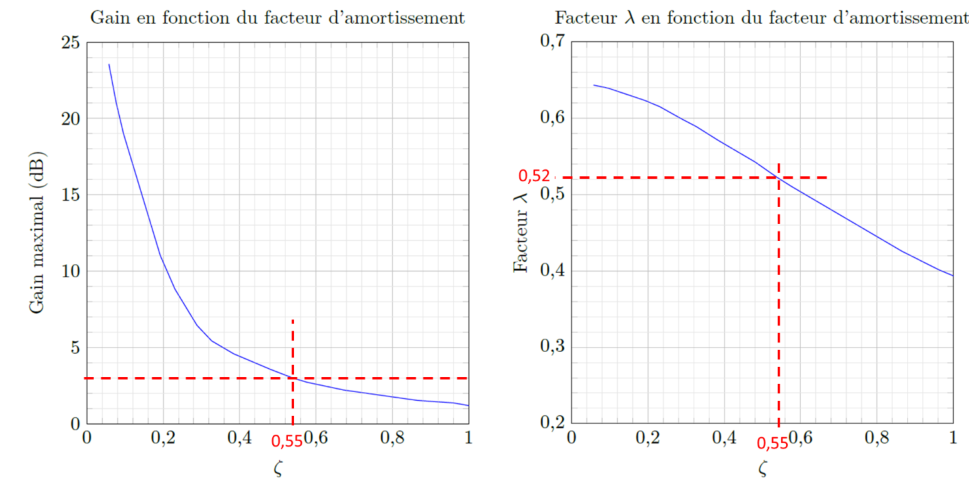
\includegraphics[width=0.85\linewidth]{Q15}
%\end{figure} 
%
%Par lecture graphique : $\zeta =0,55$ et $\lambda (\zeta)=0,52$, soit $\omega_n=\lambda(\xi)\cdot \omega_c=0,364$ rad/s, et :
%$$V_G0=\dfrac{rA}{M}\left(\dfrac {1}{\omega_n}\right)^2 (Mg+P_{\text{atm}} A)=1,56 \ \text{m}^3.$$
%
%
%
%\end{corrige}
%\else
%\fi
%
%\ifprof
%\else
%
%Le tracé du gain réel du bateau support $B(p)=\dfrac{Y_h(p)}{Y_{\text{vague}}(p)}$ est donné sur la Figure C du document réponse.\\

On utilisera dans toute la suite la relation $\tau \omega_0= 2\zeta$.\\

\fi

%
%\begin{figure}[H]
%\centering
%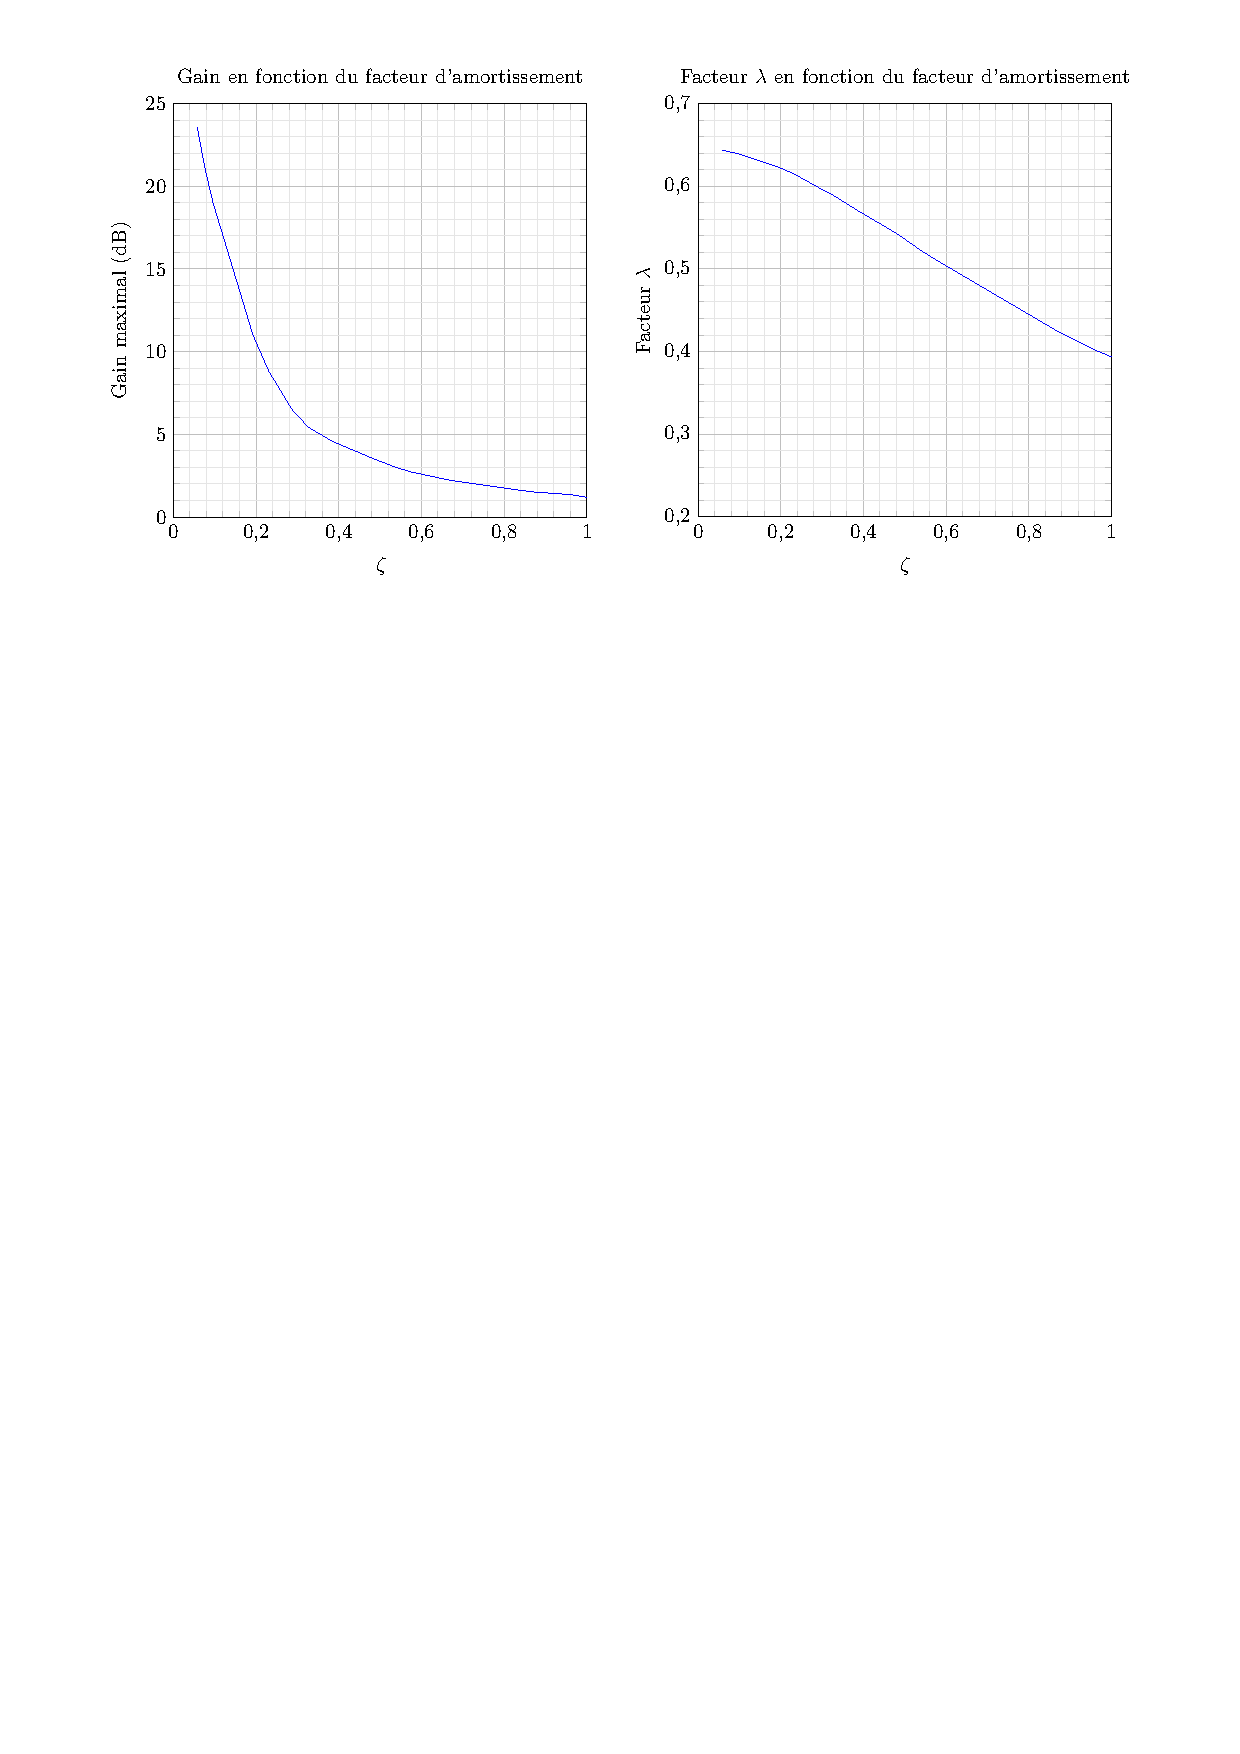
\includegraphics[width=0.8\linewidth]{Fig11}
%\caption{Courbes de détermination des facteurs du PHC}
%\label{Fig11}
%\end{figure}
%\fi




\question{Tracer en vert le diagramme asymptotique du gain de la fonction de transfert du compensateur PHC, $H(p)=\dfrac{Y_{\text{ROV}}(p)}{Y_h(p)}$, en faisant apparaître ses caractéristiques. Tracer
en bleu, sur la même figure, l’allure du gain réel du compensateur. Préciser la valeur du gain maximal.}
\ifprof
\begin{corrige}
%\textbf{Q16}  
 Diagrammes de Bode de $H(p)$. On identifie 2 pulsations caractéristiques : $\omega_1=1/\tau\approx 0,33$ rad/s et $\omega_n=0,364$ rad/s. On verra apparaître un phénomène de résonance \`a la pulsation $\omega_r=\omega_0\sqrt{1-2\zeta^2}$ car $\zeta=0,55<\sqrt{2}/2$. La résonance sera toutefois faible.

\begin{table}[H]
\begin{center}
\begin{tabular}{|c|c|c|c|}
\hline
$\omega$ & BF $\omega \ll \omega_1$ & MF $\omega_1 \ll \omega \ll \omega_n$& HF $\omega_n \ll \omega$ \\
\hline
\hline
&&&\\
$H(j\omega)$ & 1 & $\tau j \omega$ & $\dfrac{\tau\omega_n^2}{j\omega}$\\
&&&\\
\hline
&&&\\
$G_{\text{dB}}$ & 0 & $20\log\tau+20\log\omega$ & $20\log(\tau \omega_n^2)-20\log\omega$\\
&&&\\
\hline
&&&\\
$\phi$ &0 & $90^\circ$ & $-90^\circ$ \\
&&&\\
\hline
\end{tabular}
\end{center}
\end{table}



\begin{figure}[H]
\centering
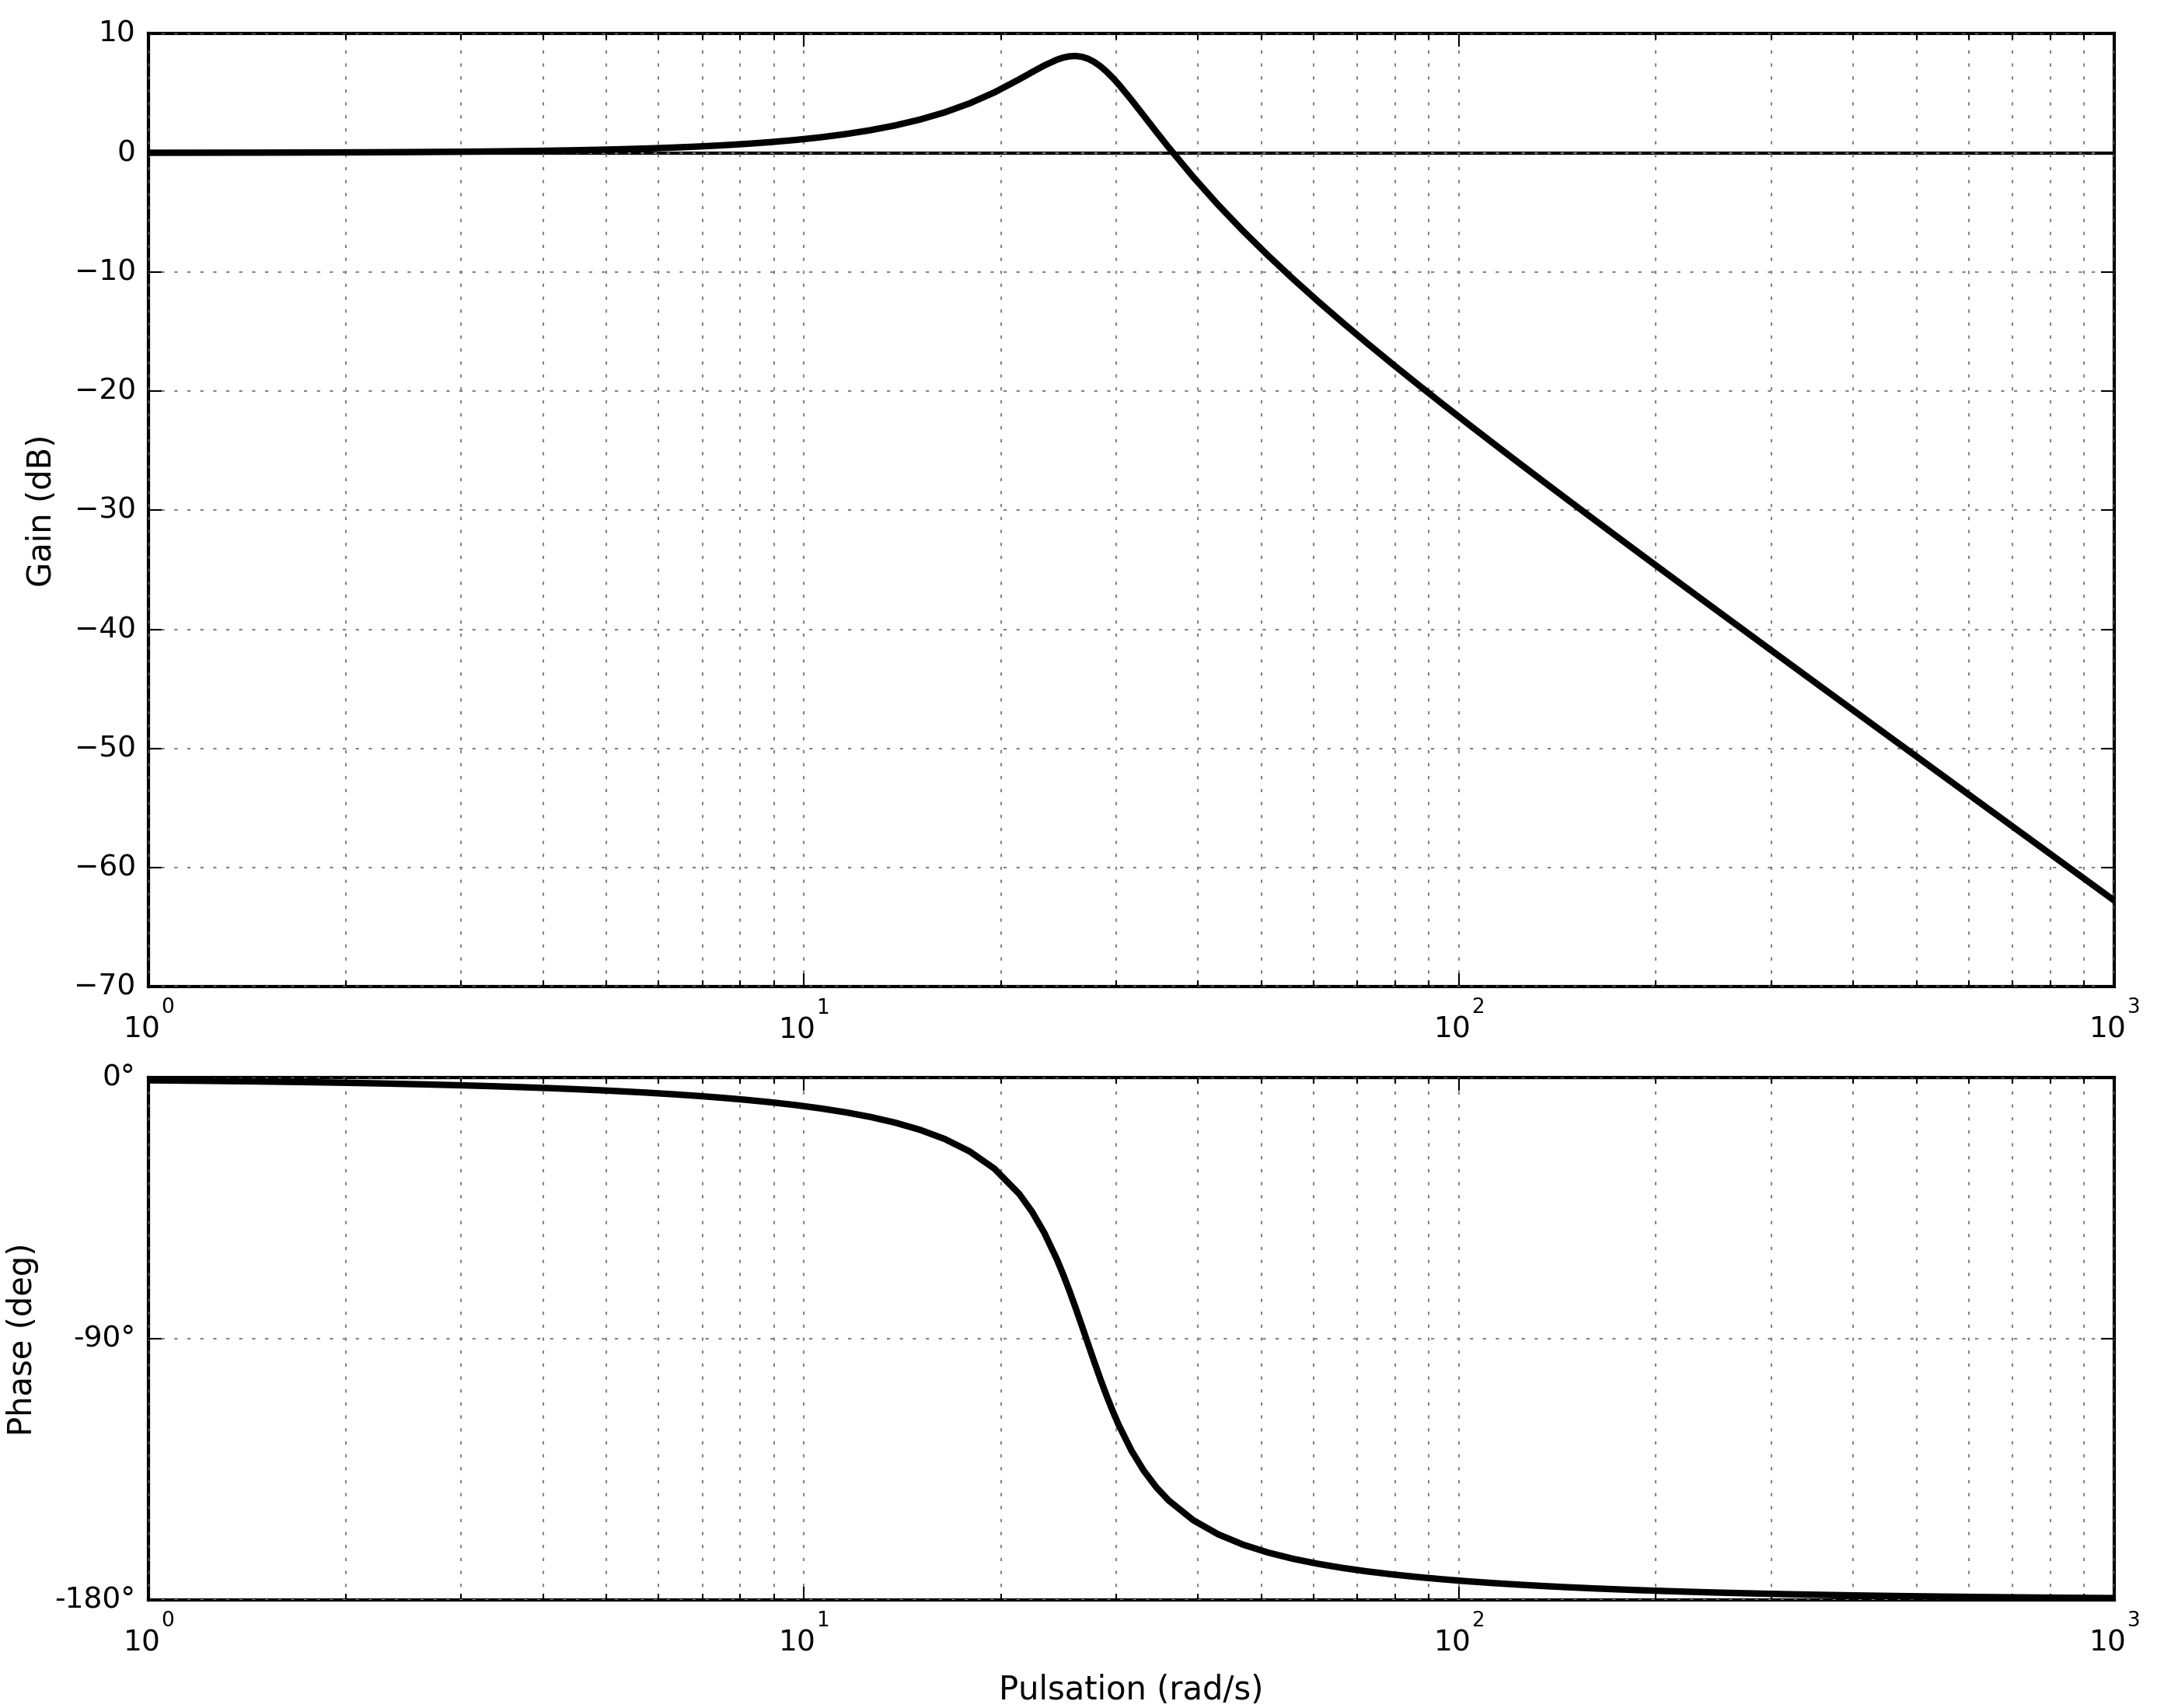
\includegraphics[width=\linewidth]{Q16}
\end{figure}


La valeur du gain maxi est de $+3$ dB (due au premier ordre au numérateur, l’influence du dénominateur est négligeable car la résonance est faible).\\

\end{corrige}
\else
\fi



\question{ Exprimer la fonction de transfert de l’ensemble \{bateau support + ROV + PHC\}, $G(p) = \dfrac{Y_{\text{ROV}}(p)}{Y_{\text{vague}}(p)}$ en fonction de $H(p)$ et $B(p)$. Tracer en rouge l'allure du gain du diagramme de Bode de $G(p)$.}
\ifprof
\begin{corrige}
%\textbf{Q17}  
On a la relation $G(p)=B(p)G(p)$. 

 \begin{figure}[H]
\centering
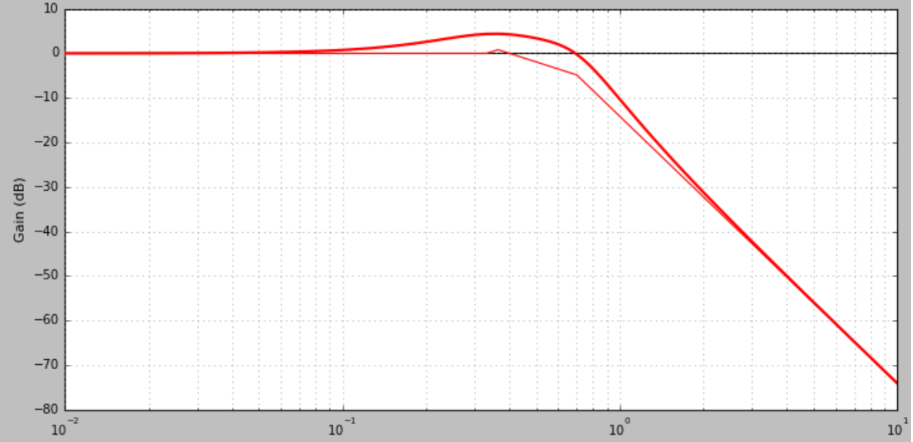
\includegraphics[width=0.75\linewidth]{Q17}
\end{figure} 


\end{corrige}
\else
\fi

\ifprof
\else
Des réglages pour différentes valeurs de pulsation de la houle $\omega_c$ et de gain maximal acceptable du compensateur ont été effectués. La \autoref{Fig12} donne les diagrammes du gain de la fonction $G(p)$ de l’ensemble \{bateau support +
ROV + PHC\} pour quatre réglages. Les volumes du gaz $V_{G0}$ correspondant à chaque réglage sont donnés dans le tableau ci-après.


\begin{figure}[H]
\centering
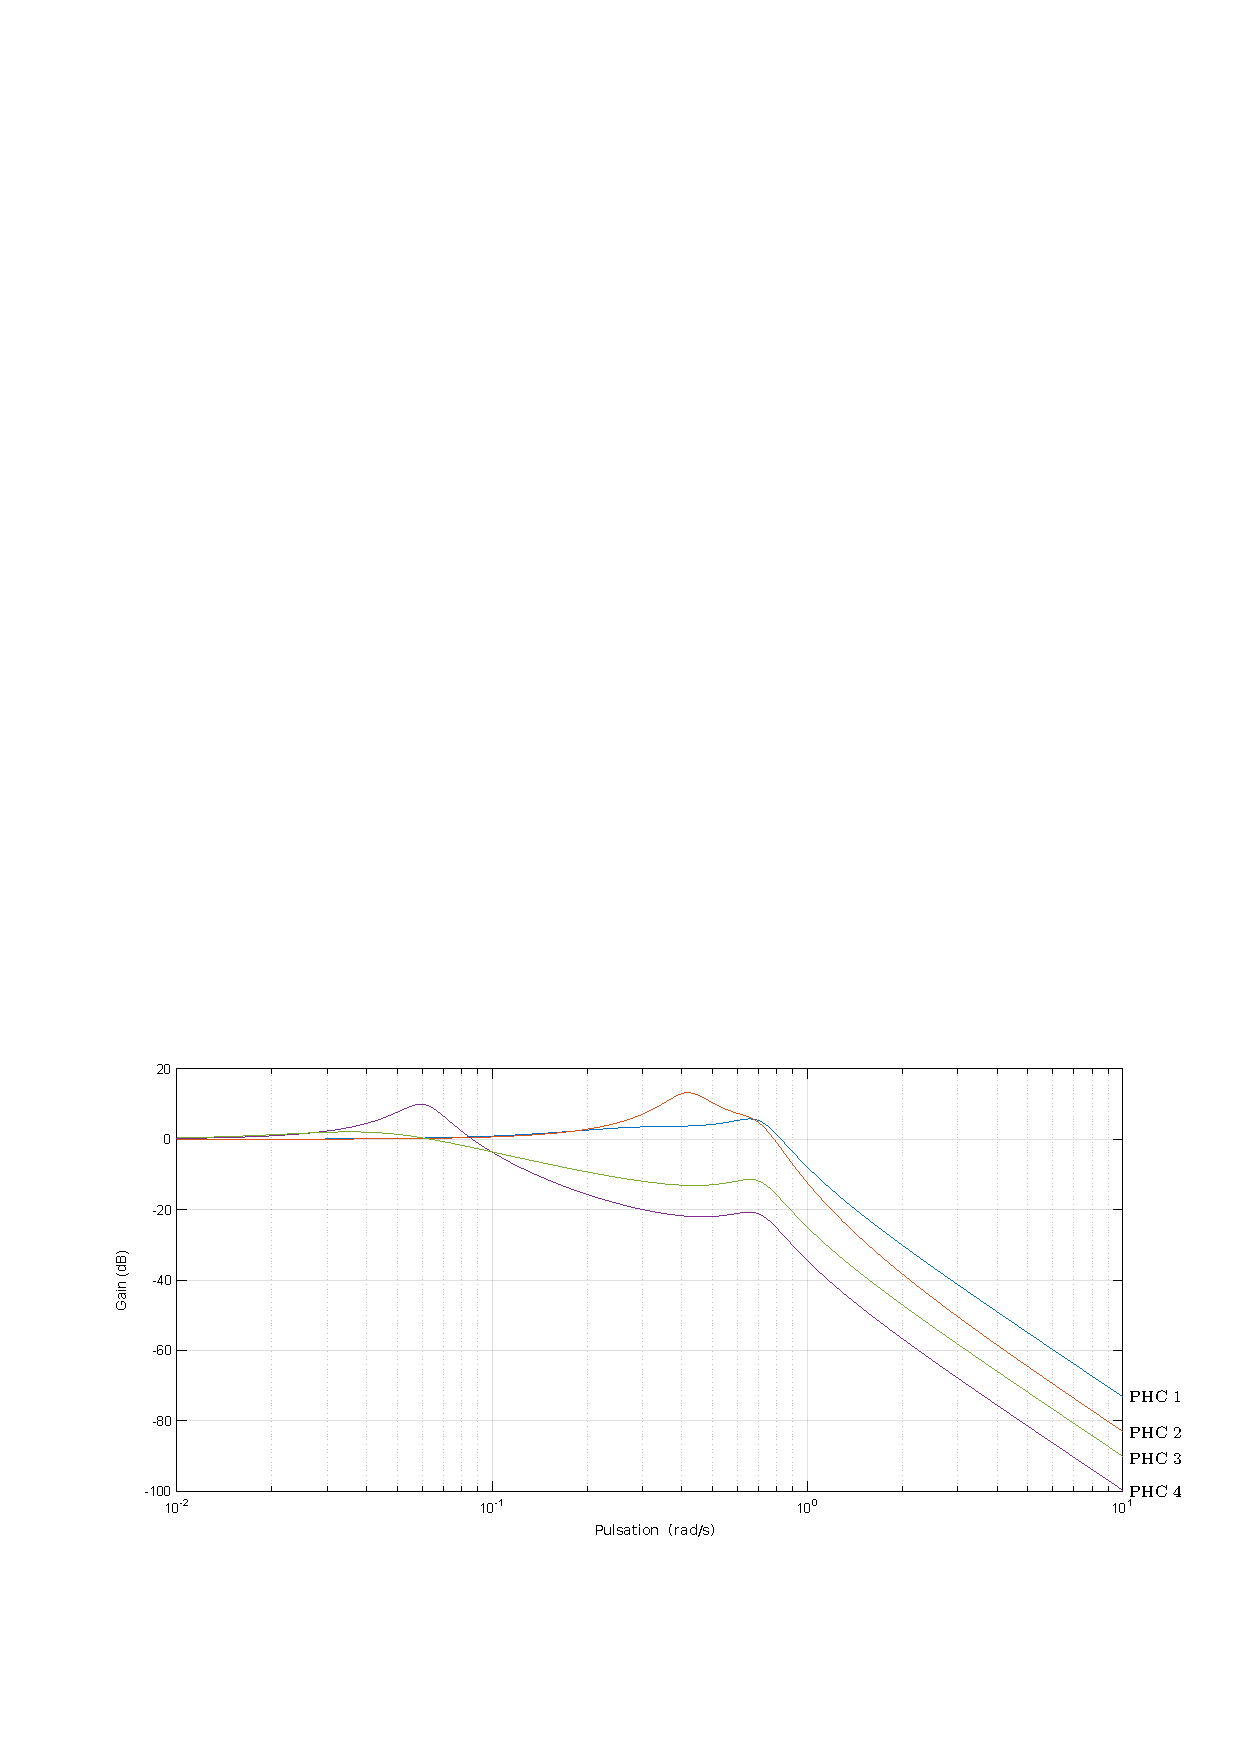
\includegraphics[width=\linewidth]{Fig12}
\caption{Courbes de gain $G(p)$ pour différents réglages du PHC}
\label{Fig12}
\end{figure}



\begin{center}
\begin{tabular}{|c|c|c|c|c|}
\hline
Réglage &PHC 1& PHC 2 &PHC 3 &PHC 4\\
\hline
\hline
$V_{G0}$ (m$^3$) &96& 1& 52& 2\\
\hline
\end{tabular}
\textit{Volumes $V_{G0}$ pour différents réglages du PHC}
\label{tab2}
\end{center}%



Pour respecter l’exigence Id 1.1, le gain de la fonction de transfert de l’ensemble doit toujours être inférieur à \SI{-14}{dB}.\\


\fi

\question{Choisir, en justifiant la réponse, le réglage du compensateur adapté à l’exigence Id 1.1.}
\ifprof
\begin{corrige}
%\textbf{Q18} 
Le réglage de PHC 4 est celui qui respecte le mieux l’exigence Id1.1. 

\begin{figure}[H]
\centering
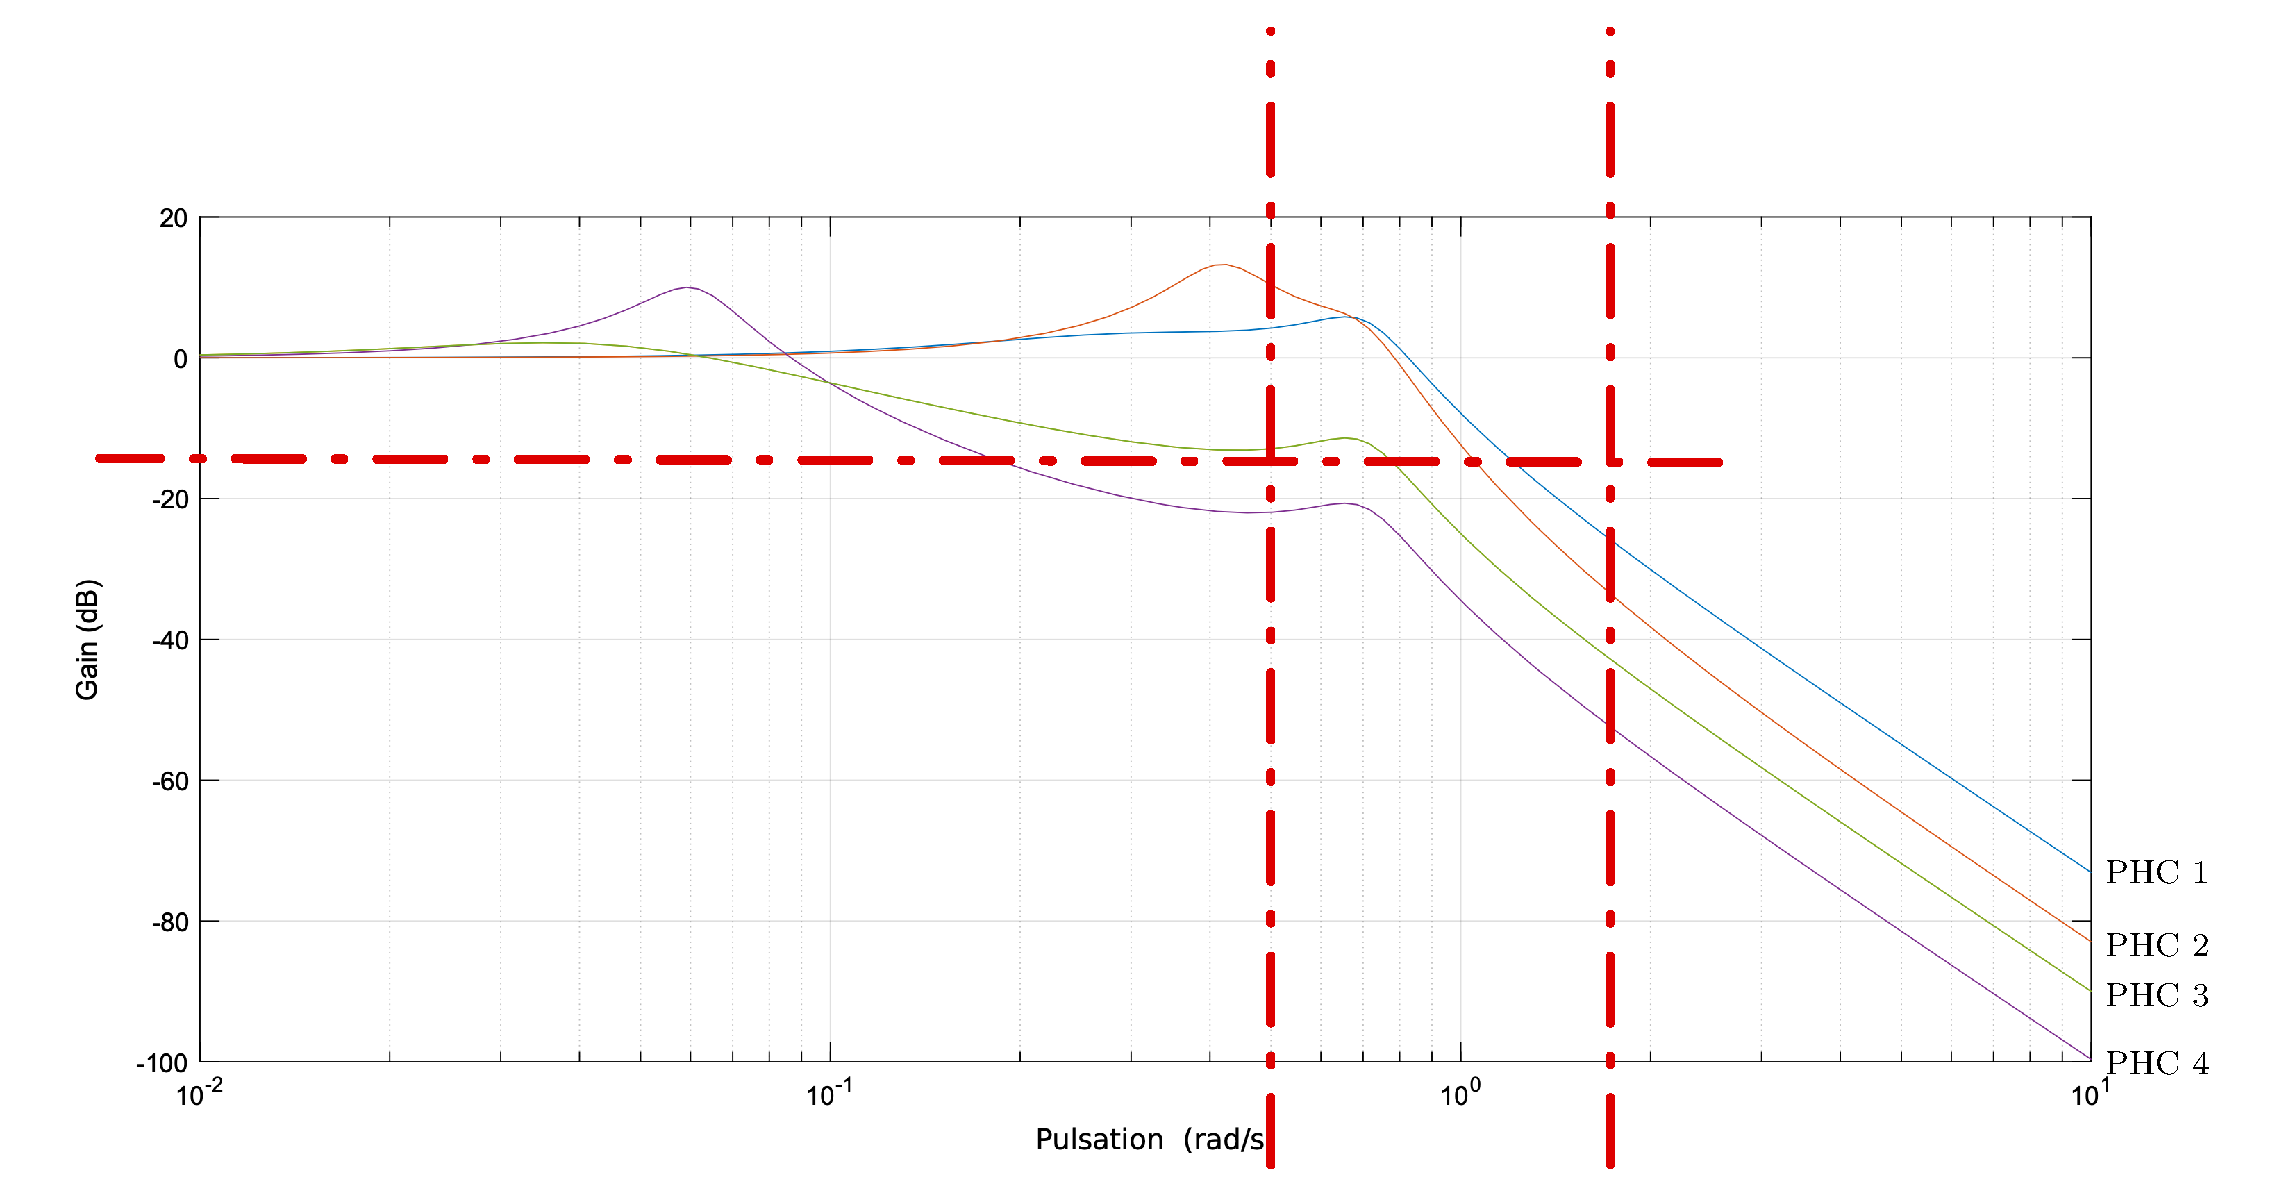
\includegraphics[width=0.85\linewidth]{Q18}
\end{figure}


\end{corrige}
\else
\fi


%Le système passif avec un réglage précis pour une pulsation de houle ne donne pas satisfaction pour tous les
%types de houle, le constructeur souhaite mettre en {\oe}uvre un système actif pour avoir une meilleure adaptabilité
%aux conditions de mer.
%
%\section{Étude du système actif de compensation de houle AHC (Active
%Heave Compensator)}
%
%
%\begin{obj}
%Dimensionner un système actif de compensation de la houle et valider sa conformité aux exigences du
%cahier des charges.
%\end{obj}
%%\textbf{Objectif} \\
%
%\ifprof
%\else
%Une solution de compensation par motorisation asservie du tambour d’enroulement est envisagée (\autoref{Fig13}). Ce
%système est un compensateur de houle actif noté AHC. Le principe est de maintenir constante la tension dans le
%câble ombilical : les vagues, par l’accélération verticale qu’elles donnent au bateau support, créent des tensions
%dans le câble ombilical qui viennent s’ajouter à celles exercées par le poids du ROV. Le principe est d’enrouler
%et dérouler le tambour d’enroulement pour compenser les variations de hauteur, donc de tension dans le câble.
%
%\begin{figure}[H]
%\centering
%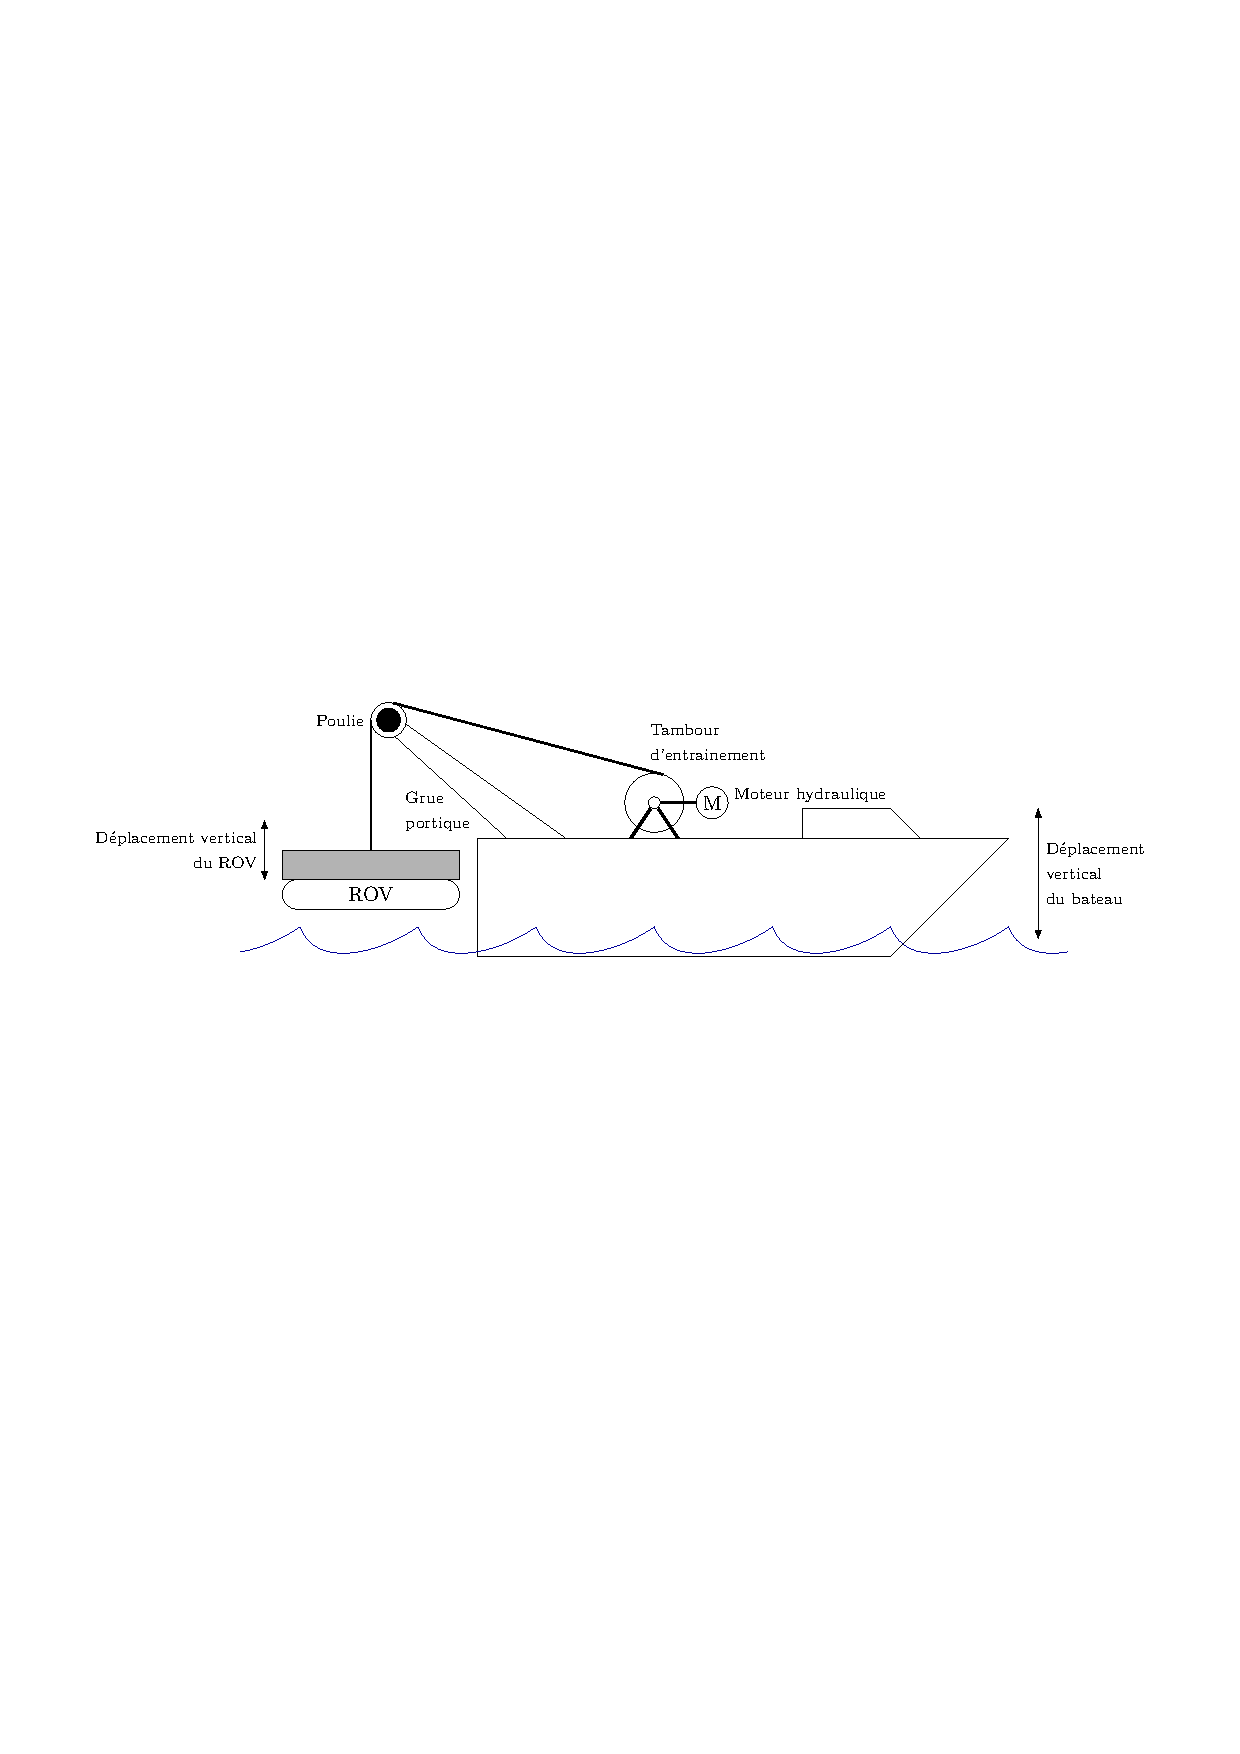
\includegraphics[width=0.95\linewidth]{Fig13}
%\caption{Schéma d’implantation du système de compensation actif}
%\label{Fig13}
%\end{figure}
%
%
%Le tambour d’enroulement est actionné par un moteur hydraulique piloté par une servo-pompe. Un capteur d’efforts mesure la tension du câble et transmet l’information à un calculateur. Un réducteur est placé entre le
%moteur et le tambour d’enroulement. Les vagues créent une perturbation dynamique modifiant la tension du
%câble.\\
%
%\textbf{Données du système }
%\begin{itemize}
%\item une servo-pompe modélisée par un système linéaire de gain $K_{sv}$ ;
%\item un moteur, de cylindrée $c$, accouplé à un réducteur de rapport de réduction $k=\dfrac{\omega_{\text{tambour}}}{\omega_{\text{moteur}}}<1$ ;
%\item un capteur d’effort linéaire de gain $K_{\text{capt}}$ ;
%\item un volume du circuit hydraulique $V$ ;
%\item un coefficient de raideur hydraulique $\beta$ ;
%\item une inertie équivalente ramenée à l’axe moteur notée $J_{\text{eq}}$ {(à calculer)} ;
%\item un diamètre d’enroulement maximal du câble $D_{\text{max}} = 1800$ mm ;
%\item  un diamètre d’enroulement minimal du câble $D_{\text{min}} = 1300$ mm ;
%\item une poulie de guidage du câble d’inertie autour de son axe de rotation $J_{\text{poulie}} = 200 \ \text{kg}\cdot \text m^2$ ;
%\item la position angulaire du tambour est notée $\alpha_T$ ;
%\item la position angulaire du moteur est notée $\theta_m$ ;
%\item la masse du ROV, {$M_{\text{ROV}} = 13$ t}.
%\end{itemize}
%
%
%\textbf{Équations hydrauliques}
%\begin{itemize}
%\item la relation entre le débit moteur $(Q_m)$, la pression moteur ($P_m$) et le débit de la pompe ($Q_p$) est donnée par la relation $Q_m=Q_p+\dfrac{\text dV}{\text dt}-\dfrac{V}{\beta}\dfrac{\text dP_m}{\text dt}$ ;
%\item les circuits hydrauliques (corps de vérin, moteur et élément du circuit hydraulique) sont très rigides, on néglige donc la variation de volume des enceintes devant celle du fluide, $\dfrac{\text dV}{\text dt}=0$ ;
%\item le couple moteur est obtenu par la relation $C_m = cP_m$ ;
%\item le débit traversant le moteur est obtenu par la relation $Q_m = c\dfrac{\text d\theta_m}{\text dt}$.
%\end{itemize}
%
%Dans cette étude, le repère lié au bateau est considéré galiléen. Les effets des accélérations verticales seront pris
%en compte dans la perturbation notée $F_{\text{pert}}(p)$ représentée par un effort sinusoïdal lié aux accélérations verticales
%du bateau.\\
%
%%L’ensemble \{tambour + câble\} est modélisé par un cylindre creux en acier de masse volumique $\rho = 7200 \ \text{kg}\cdot \text m^{-3}$,
%%de rayon extérieur $R_{\text{max}} = 1$ m, de rayon intérieur $R_{\text{min}} = 0,65$ m et de longueur $L = 1600$ mm. On notera $M_{\text{tamb}}$ la masse du cylindre creux modélisant l’ensemble \{tambour + câble\}. L’inertie de l’ensemble \{tambour + câble\} modélisé est {$I_{\text{tamb}} =\dfrac{L}{2}\rho \pi (R^4_{\text{max}}-R^4_{\text{min}})$}. %(\textcolor{red}{erreur  d'énoncé $I_{\text{tamb}} =\dfrac{L}{2}\rho \pi (R^4_{\text{max}}-R^4_{\text{min}})$}).
%%%\\
%%
%%\begin{figure}[H]
%%\centering
%%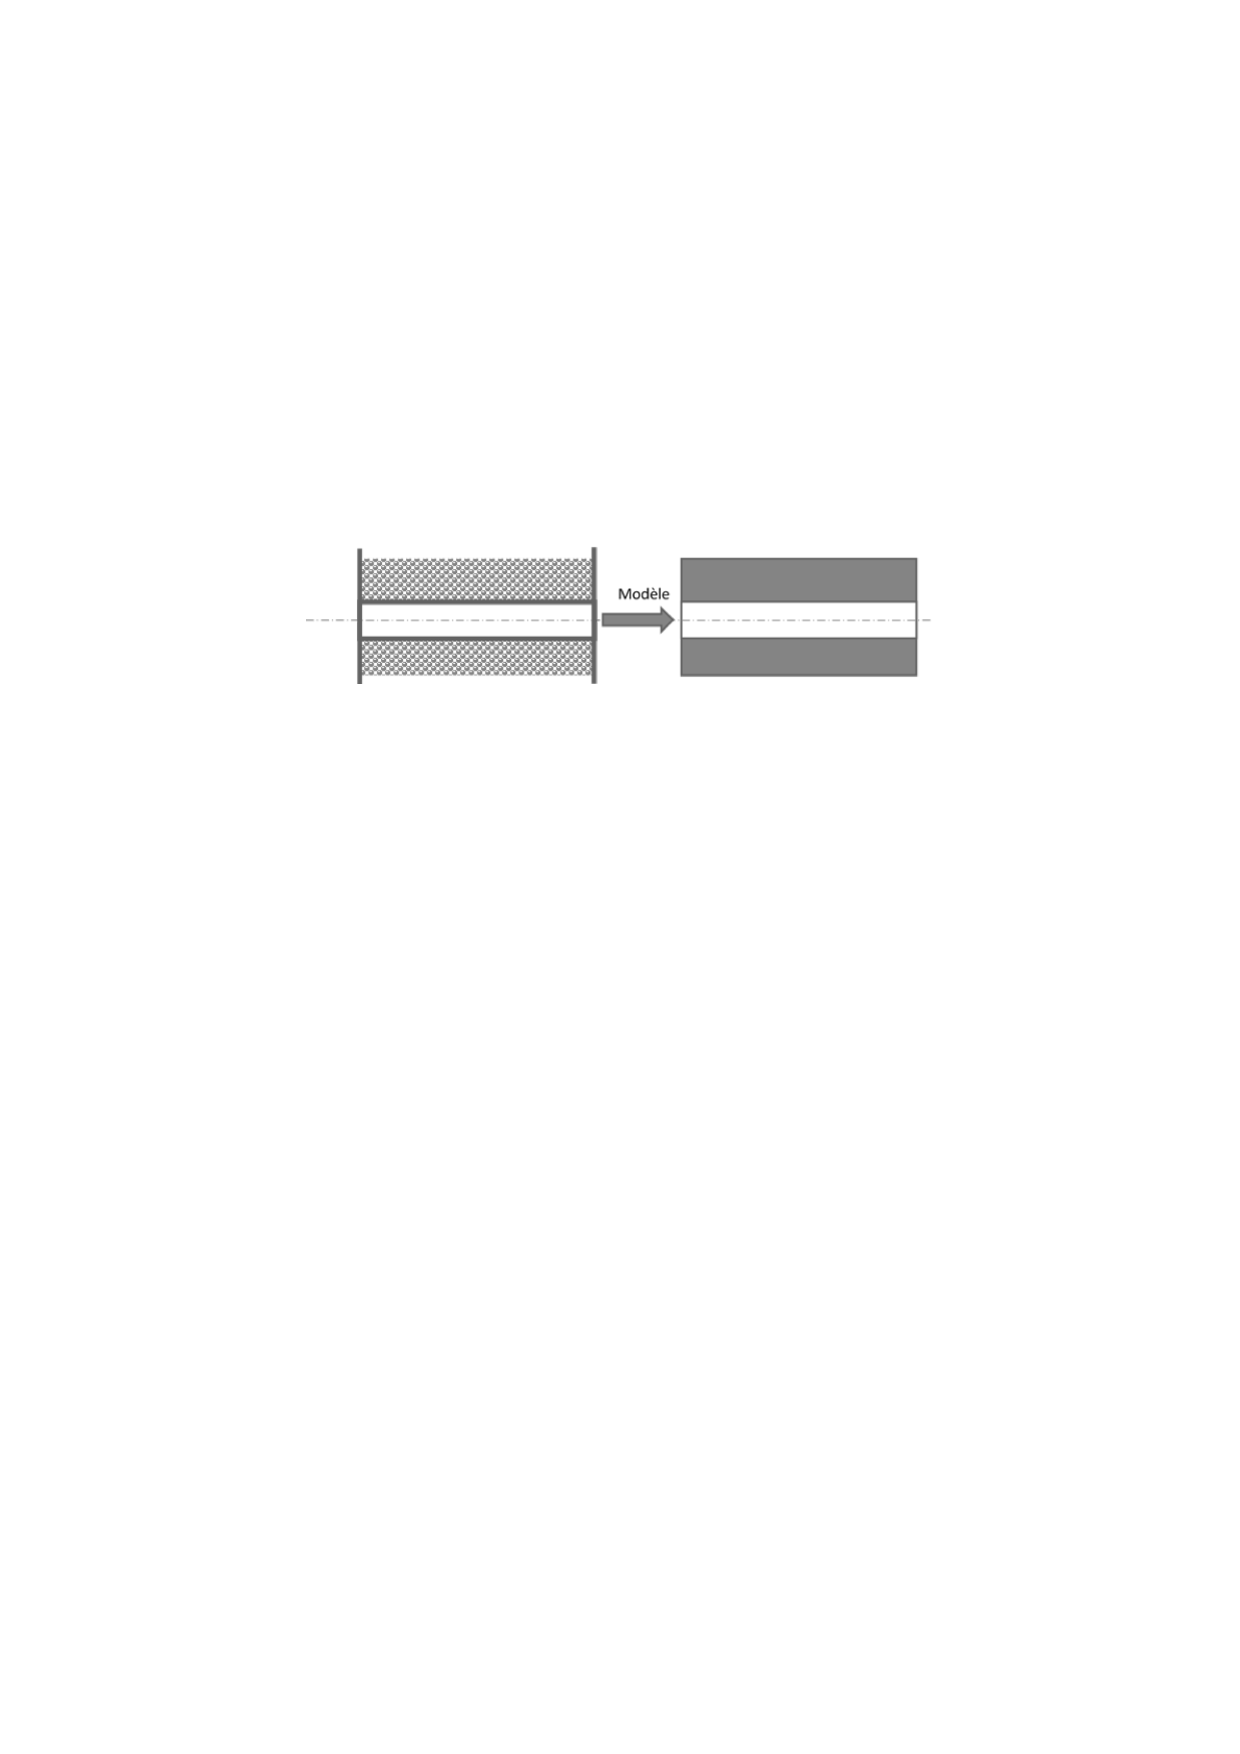
\includegraphics[width=0.75\linewidth]{Fig14}
%%\caption{Modélisation du tambour et du câble enroulé}
%%\label{Fig14}
%%\end{figure}
%%
%%
%%\fi
%%
%%
%%\question{Ne pas traiter -- Après avoir exprimé $I_{\text{tamb}}$ en fonction de $M_{\text{tamb}}$, $R_{\text{max}}$ et $R_{\text{min}}$, déterminer l’inertie équivalente notée $I_{\text{eq}}$ ramenée sur l’arbre moteur de l’ensemble $E =$ \{tambour + poulie + ROV\} lorsque le diamètre d’enroulement
%%est égal à $D_{\text{max}}$. La masse du câble déroulé sera négligée devant la masse du ROV et on admet que la poulie de guidage tourne à la même vitesse angulaire que le tambour. }
%%\ifprof
%%\begin{corrige}
%%%\textbf{Q19} 
%%\textcolor{red}{Erreur d'énoncé} 
%%
%%$I_{\text{tamb}}=\dfrac{L}{2}\rho \pi (R^4_{\text{max}}-R^4_{\text{min}})$ avec $M_{\text{tamb}}=\rho \pi (R^2_{\text{max}}-R^2_{\text{min}}).$
%%
%%
%%Soit : $I_{\text{tamb}}=\dfrac{L}{2}\rho \pi (R^2_{\text{max}}-R^2_{\text{min}})(R^2_{\text{max}}+R^2_{\text{min}})$.
%%
%%Donc $\boxed{I_{\text{tamb}}=\dfrac{1}{2}M_{\text{tamb}}(R^2_{\text{max}}+R^2_{\text{min}}).}$\\
%%
%%On calcule l'énergie cinétique de l'ensemble $E$ :
%%
%%\begin{eqnarray}
%%T_{E/\mathcal R_0}&=&T_{\text{ROV}/\mathcal R_0}+T_{\text{poulie}/\mathcal R_0}+T_{\text{tambour}/\mathcal R_0},\nonumber \\
%%T_{E/\mathcal R_0}&=& \dfrac{1}{2}M_{\text{ROV}}\overrightarrow V_{\text{ROV}/\mathcal R_0}^2 +\dfrac{1}{2}J_{\text{poulie}} \dot \alpha_T^2+\dfrac{1}{2}I_{\text{tamb}}\dot \alpha_T^2,\nonumber
%%\end{eqnarray}
%%avec $\overrightarrow V_{ROV/\mathcal R_0}=R_{\text{max}}k\dot \theta_m$ et $\dot \alpha_T=k\dot \theta_m$. On obtient :
%%
%%$$T_{E/\mathcal R_0}=\dfrac{k^2}{2}\left(M_{\text{ROV}}R_{\text{max}}^2+J_{\text{poulie}} +I_{\text{tamb}}\right)\dot \theta_m^2.$$
%%
%%Ainsi :
%%
%%$$\boxed{I_{eq}=M_{\text{ROV}}k^2R_{\text{max}}^2+(J_{\text{poulie}}+I_{\text{tamb}})k^2.}$$
%%
%%
%%
%%\end{corrige}
%%\else
%%\fi
%%
%%
%%\question{Ne pas traiter -- Déterminer l’expression du couple moteur $C_m$ par application du théorème de l’énergie cinétique
%%appliqué à $E$ en phase de montée du ROV. Le bilan des puissances sera détaillé.}
%%\ifprof
%%\begin{corrige}
%%%\textbf{Q20} 
%%On isole l'ensemble $E$ et on applique le TEC :
%%$$\dfrac{\text dT_{E/\mathcal R_0}}{\text dt}=\sum \mathcal P_{\text{ext}\to E}+\sum \mathcal P_{\text{int}}.$$
%%
%%On dresse le bilan des puissances des efforts extérieurs agissant sur $E$ dans son mouvement par rapport au repère galiléen $\mathcal R_0$ :
%%\begin{itemize}
%%\item $\mathcal P_{\text{pes}\to \text{ROV}/\mathcal R_0}=-MgR_{\text{max}}k\dot \theta_m$ ;
%%\item $\mathcal P_{\text{pes}\to \text{poulie}/\mathcal R_0}=0$ car le poids passe par l'axe de rotation ;
%%\item $\mathcal P_{\text{pes}\to \text{tambour}/\mathcal R_0}=0$ car le poids passe par l'axe de rotation ;
%%\item $\mathcal P_{\text{pes}\to \text{cable}/\mathcal R_0}=0$ car la masse du cable est négligeable ;
%%\item $\mathcal P_{\text{mot}\to E/\mathcal R_0}=C_m\dot \theta_m$.
%%\end{itemize}
%%
%%La puissance des inter-efforts est nulle $\mathcal P_{\text{int}}=0$ car les liaisons sont parfaites. 
%%
%%
%%Ainsi $I_{\text{eq}}\dot \theta_m\ddot \theta_m=C_m\dot \theta_m-M_{\text{ROV}}gR_{\text{max}}k \dot \theta_m$ et :
%%$$\boxed{C_m=I_{\text{eq}}\ddot \theta_m +M_{\text{ROV}}gR_{\text{max}}k.}$$
%%
%%
%%\end{corrige}
%%\else
%%\fi
%%
%%
%%
%%\ifprof
%%\else
%%L'application du théorème de l’énergie cinétique appliqué à $E$ en phase de montée du ROV permet de montrer que $C_m = I_{\text{eq}}\ddot{\theta}_m+M_{\text{ROV}}g R_{\text{max}}k$.
%%
%%Les équations du modèle de connaissance étant déterminées, on souhaite construire un modèle de simulation du système de compensation actif. On note $T_c(p)$ la consigne de tension du câble souhaitée, égale au poids statique du ROV, et $T (p)$ la tension du câble en sortie.
%%
%%\begin{figure}[H]
%%\centering
%%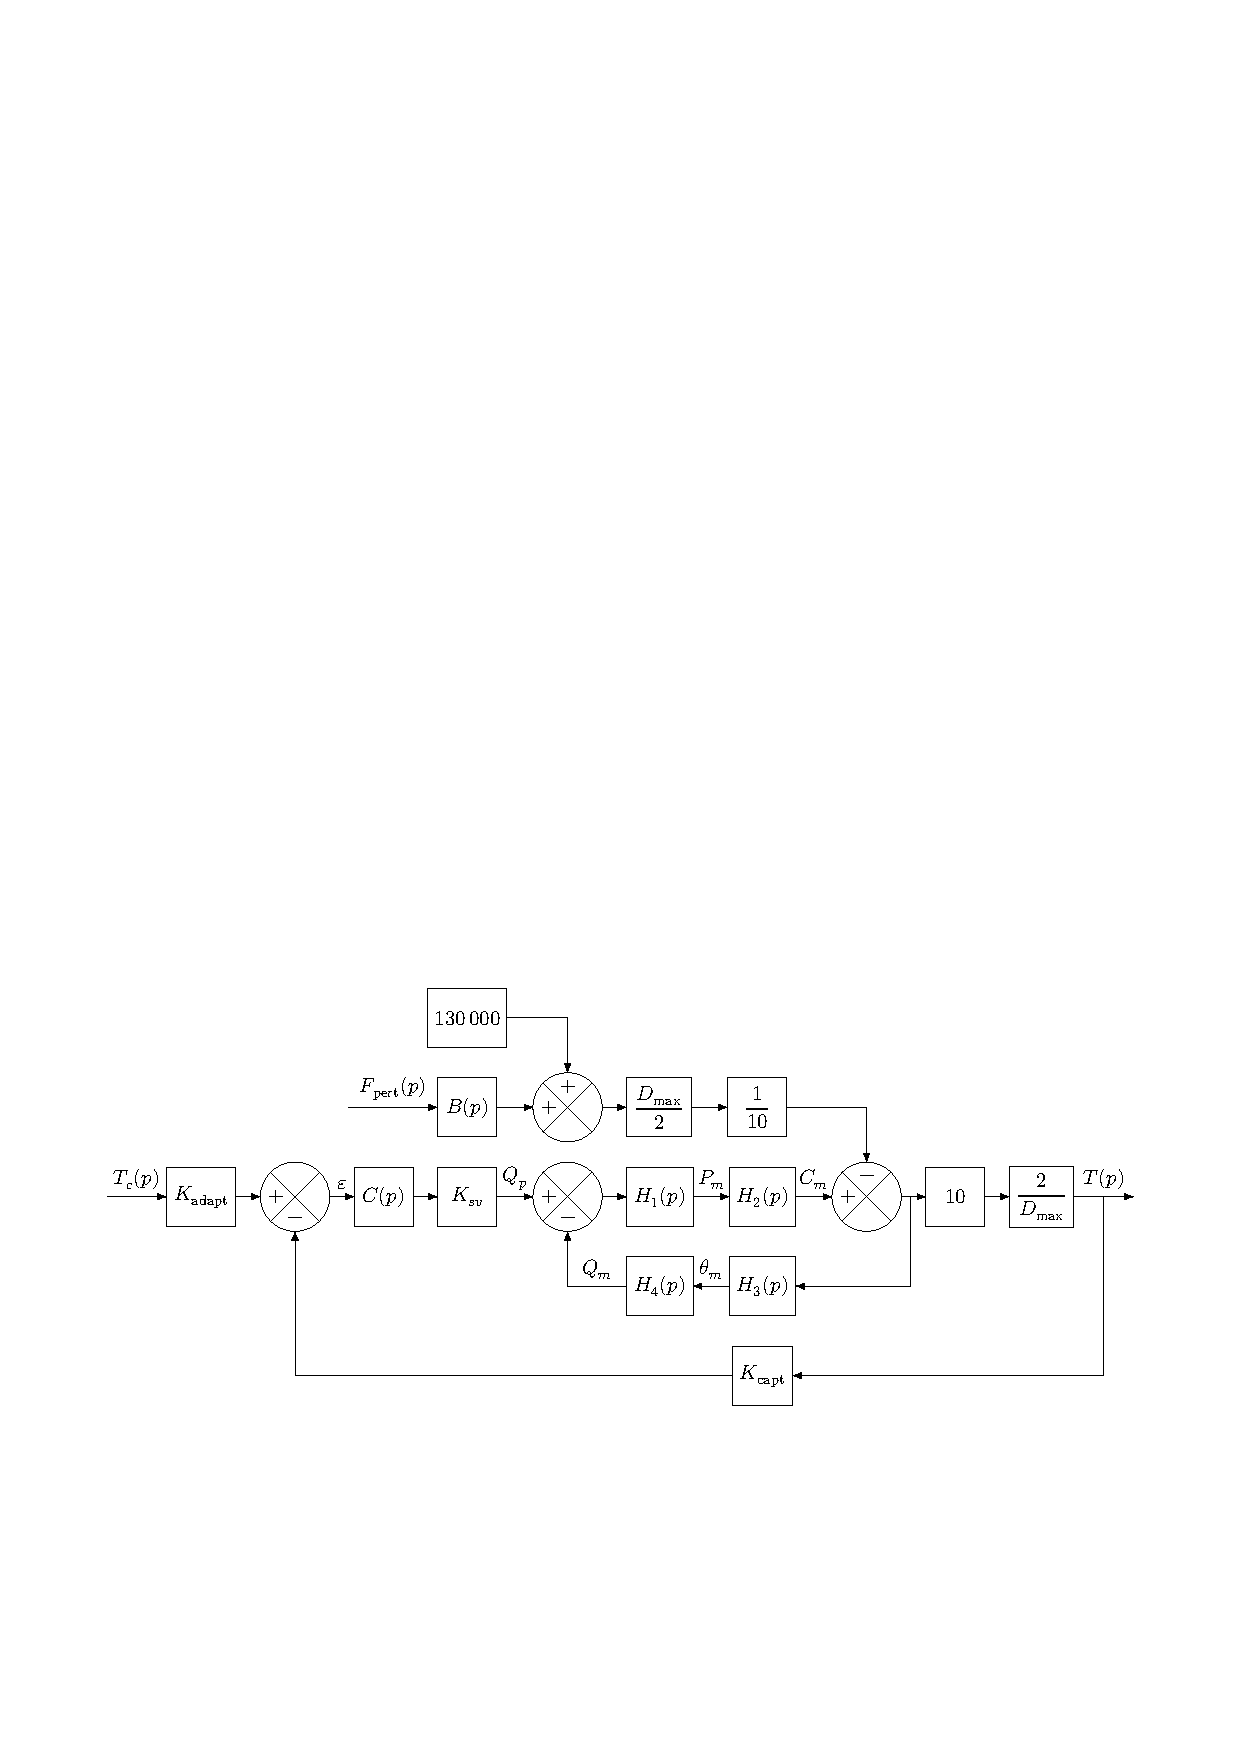
\includegraphics[width=0.8\linewidth]{Fig15}
%%\caption{Modélisation causale du système \{treuil + ROV\}}
%%\label{Fig15}
%%\end{figure}
%%
%%\fi
%
%
%\question{À partir des équations données précédemment et après avoir appliqué les transformées de Laplace en
%considérant les conditions initiales nulles, déterminer les fonctions de transfert $H_i(p)$ ainsi que $K_{\text{adapt}}$ définis sur le schéma bloc \autoref{Fig15} pour que l’écart $\varepsilon(p)$ soit l’image de l’erreur $T_c(p) -T (p)$.}
%\ifprof
%\begin{corrige}
%%\textbf{Q21}   
%On écrit les équations données dans le domaine de Laplace :
%\begin{eqnarray}
%I_{\text{eq}} p^2\theta_m(p)&=&C_m(p)-M_{\text{ROV}}gkR_{\text{max}}, \nonumber\\
%Q_{p}(p)-Q_{m}(p)&=&\dfrac{V}{\beta}pP_m(t),\nonumber\\
%C_m(p) &=& cP_m(p),\nonumber\\
%Q_m(p) &=& cp\theta_m(p).\nonumber
%\end{eqnarray}
%
%On obtient :
%$$\boxed{H_1(p)=\dfrac{\beta}{Vp} \ \; \ \ H_2(p)=c \ \; \ \ H_3(p)=\dfrac{1}{J_{eq}p^2} \ \ ; \ \ H_4(p)=cp.}$$
%
%De plus $K_{\text{adapt}}=K_c$.\\
%\end{corrige}
%\else
%\fi
%
%
%
%\ifprof
%\else
%On propose d’utiliser un correcteur de type proportionnel $C(p) = K_p$.
%Le résultat de la simulation numérique a permis de tracer les diagrammes de Bode de la \autoref{Fig16} pour différentes
%valeurs du correcteur $C(p)$ ainsi que les réponses temporelles données \autoref{Fig17}.
%
%\begin{figure}[H]
%\centering
%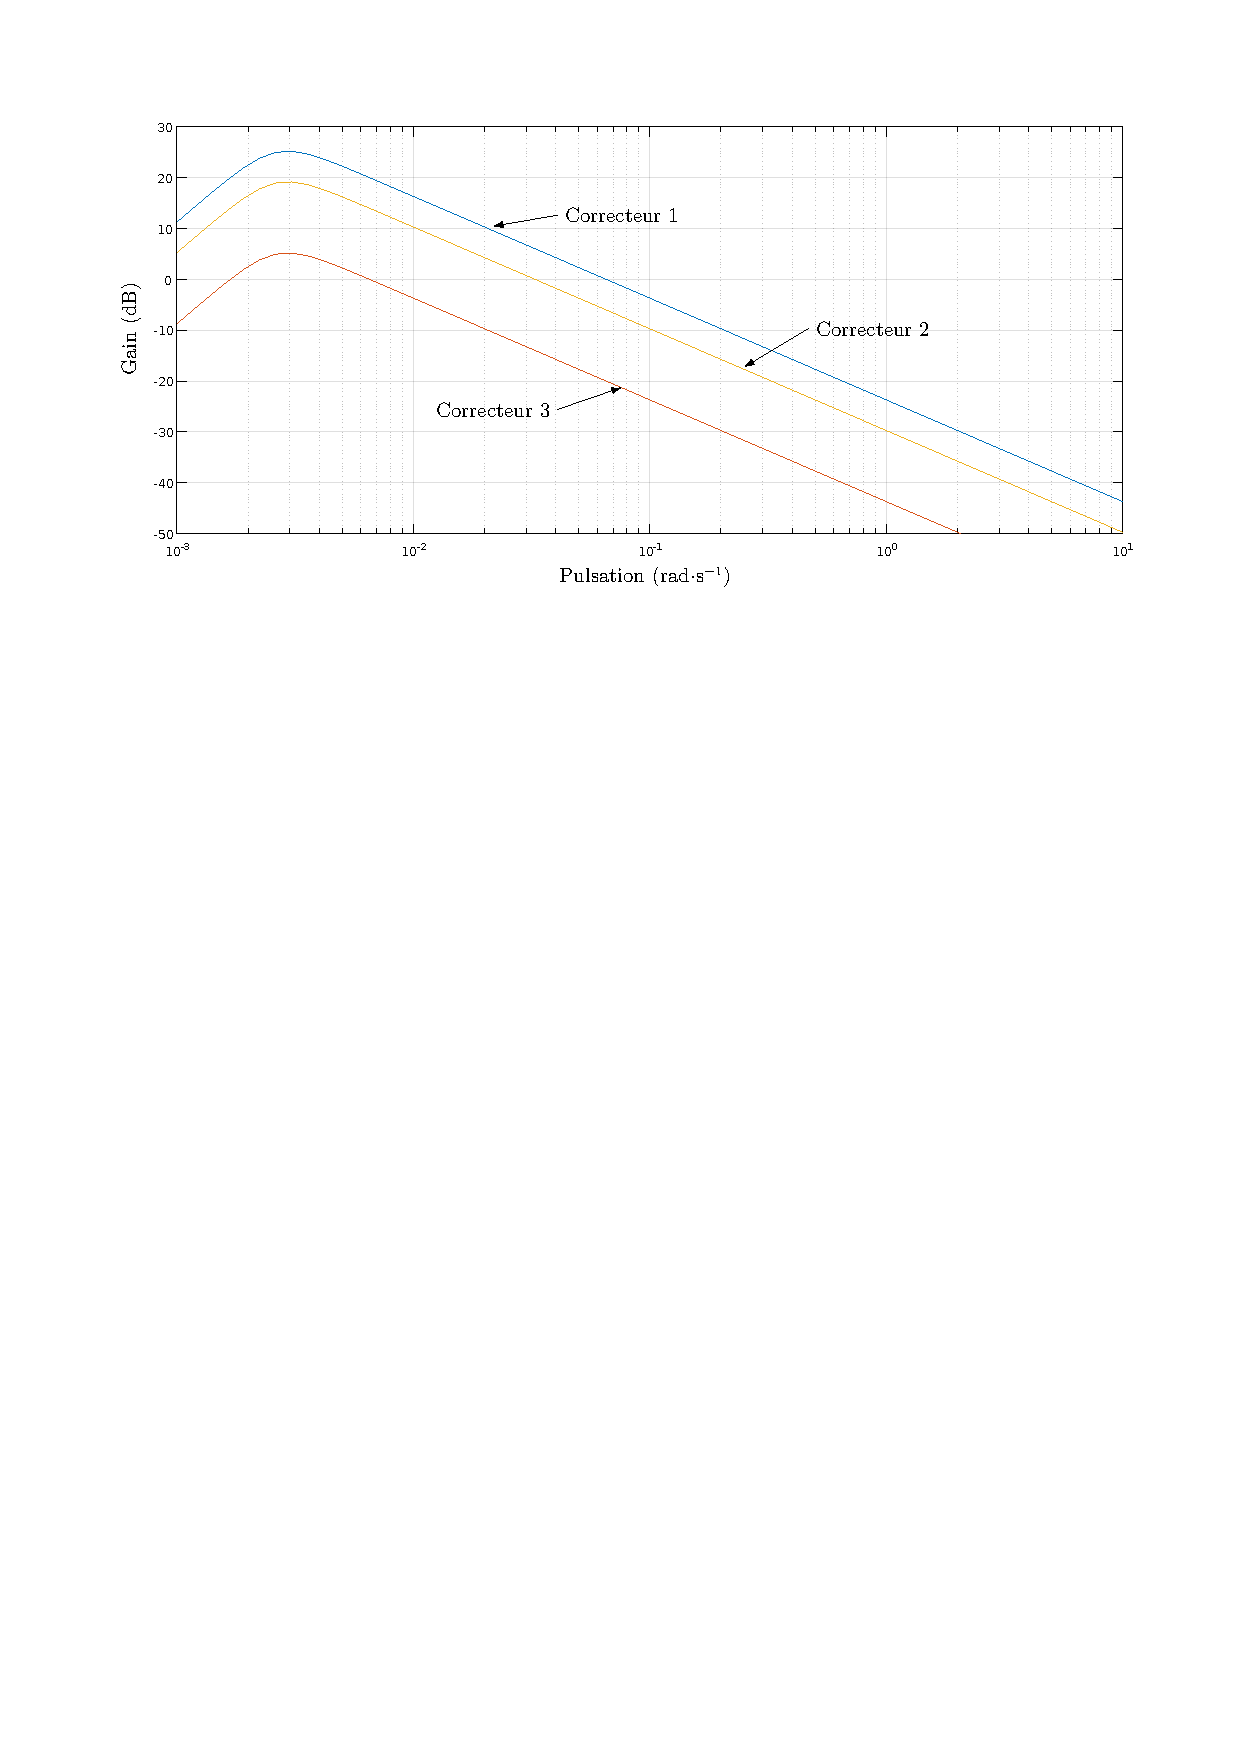
\includegraphics[width=0.8\linewidth]{Fig16}
%\caption{Diagramme de Bode en gain du système actif en boucle fermée de fonction de transfert $T (p)/F_{\text{pert}}(p)$ à consigne de tension constante}
%\label{Fig16}
%\end{figure}
%
%\begin{figure}[H]
%\centering
%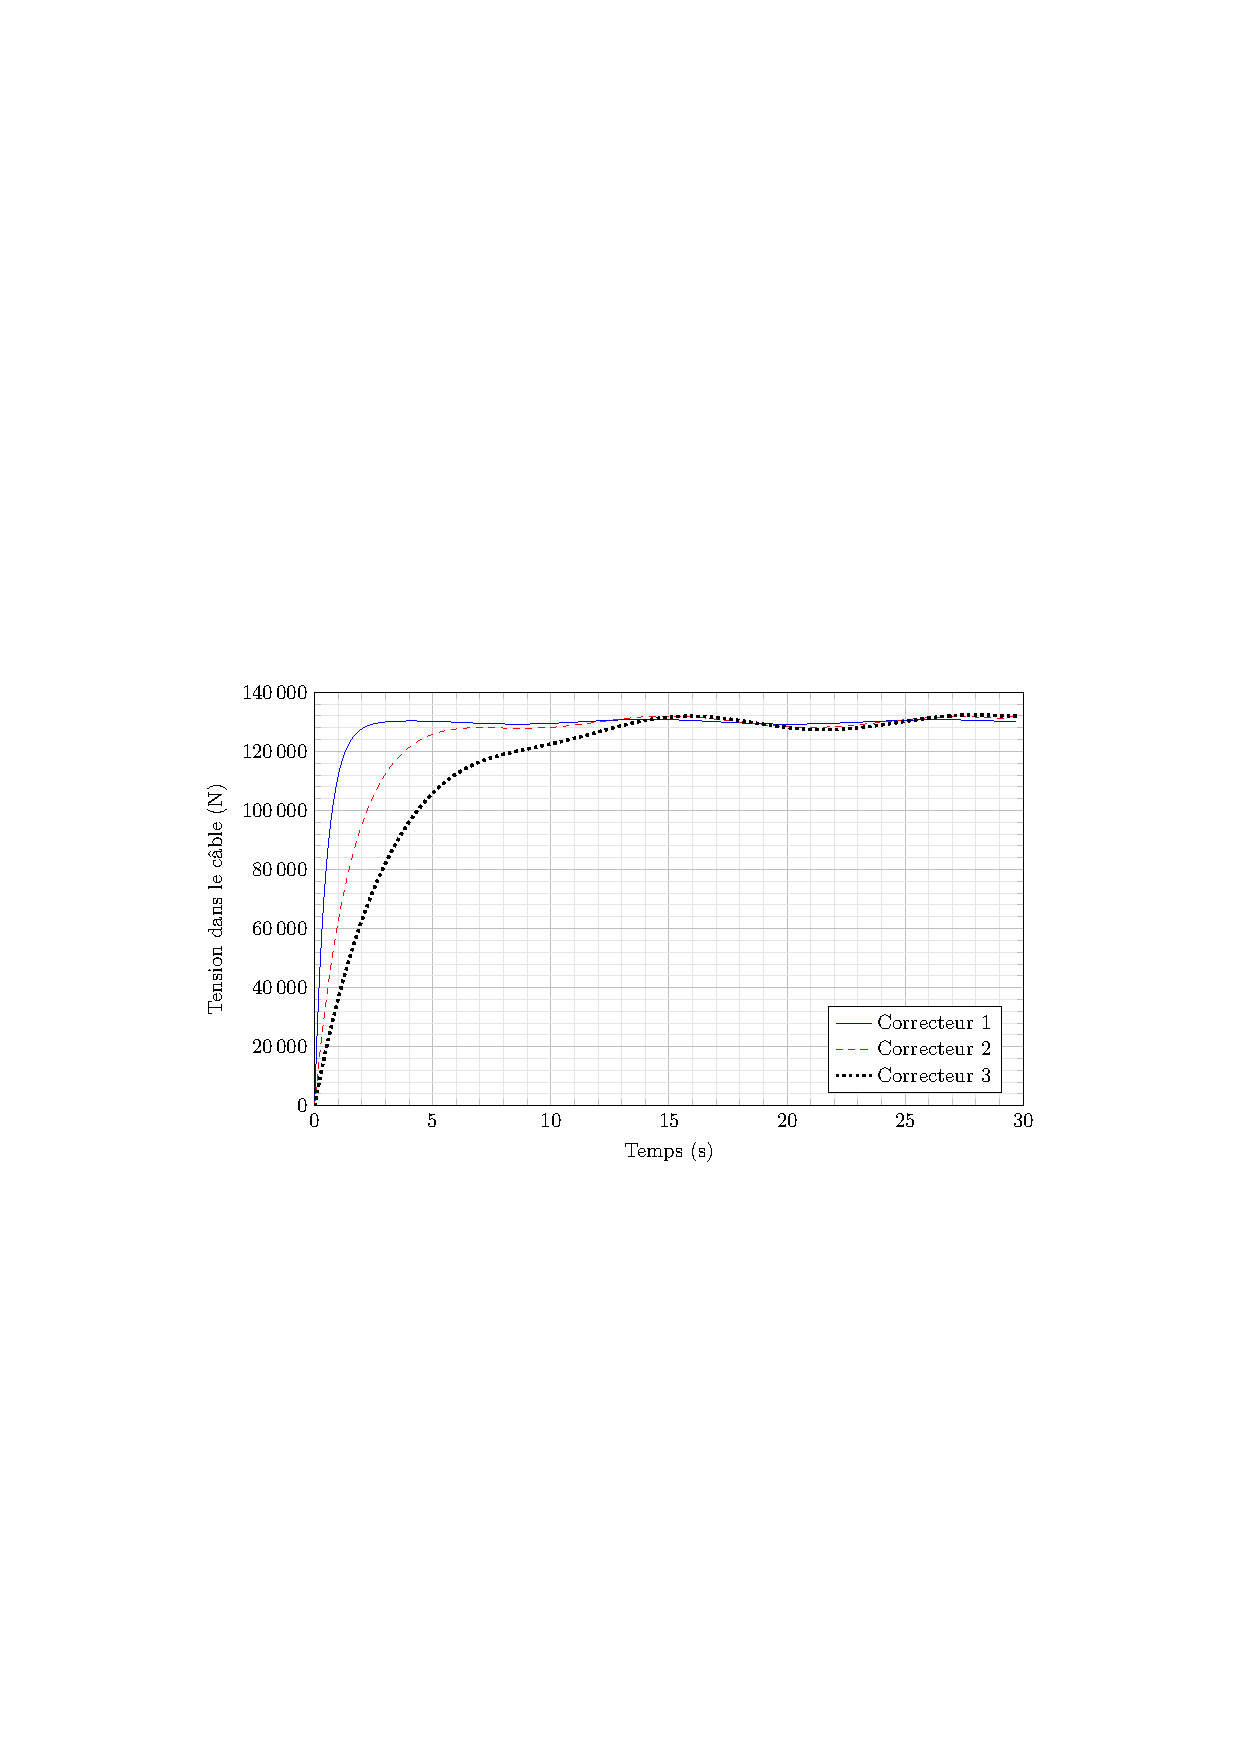
\includegraphics[width=0.8\linewidth]{Fig17}
%\caption{Réponse temporelle à un échelon d’amplitude de \SI{130 000}{N} du système actif en boucle
%fermée de fonction de transfert $T (p)/T_c(p)$ à perturbation constante}
%\label{Fig17}
%\end{figure}
%
%Le système AHC doit permettre une atténuation des effets dynamiques sur la tension du câble supérieure à \SI{15}{dB} sur la plage de pulsations de la houle comprises entre $0,5$ et $1,7 \ \text{rad}\cdot s^{-1}$ et satisfaire à l’exigence Id 1.2 du cahier des charges.\\
%
%\fi
%
%
%\question{ Par analyse des Figures \ref{Fig16} et \ref{Fig17}, choisir le correcteur du système actif le plus adapté pour satisfaire
%à l’exigence d’atténuation de \SI{15}{dB} et à l’exigence Id 1.2 du cahier des charges. Faire apparaître clairement les traits de construction sur la Figure D du document réponse. Répondre entièrement à cette question sur le document réponse.}
%\ifprof
%\begin{corrige}
%%\textbf{Q22} 
%\begin{figure}[H]
%\centering
%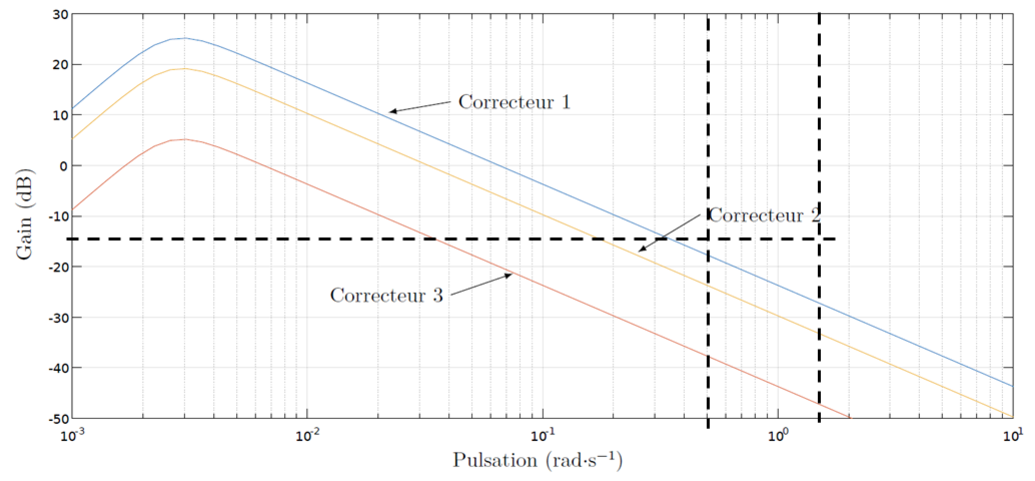
\includegraphics[width=0.85\linewidth]{Q22a}
%\end{figure}
%
%\begin{figure}[H]
%\centering
%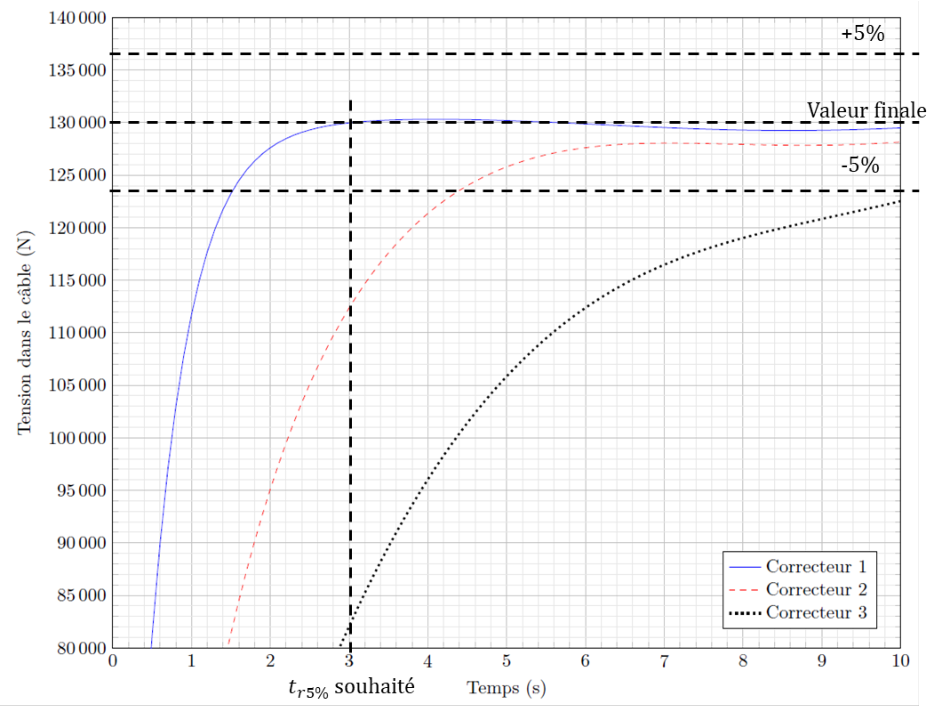
\includegraphics[width=0.85\linewidth]{Q22b}
%\end{figure}
%
%Par analyse du diagramme de Bode on voit que les trois correcteurs permettent d’atténuer de 14 dB dans la bande 0,5 rad/s à 1,7 rad/s. 
%L’exigence Id 1.2 impose un $t_{r5\%}$ de 3 s que seul le correcteur 1 permet d’obtenir. On choisit donc le correcteur 1.\\
%
%\end{corrige}
%\else
%\fi
%
%
%\ifprof
%\else
%
%
%La \autoref{Fig18} donne les courbes réelles, obtenues par mesure de la tension du câble $T(t)$, en régime stabilisé, pour une amplitude de houle de 5 m, dans les cas de l’AHC actif ou inactif.
%Dans le cas de l’AHC actif, il est possible de modéliser la tension $T(t)$ appliquée au ROV par une fonction périodique de période $T_p = 9,5$ s telle que :
%$$T(t) = 130 000 + 5500 \sin(\omega t).$$
%Dans ces conditions, on note $\Delta y(t)$ l’altitude du ROV autour de la position d’équilibre.
%
%
%
%\begin{figure}[H]
%\centering
%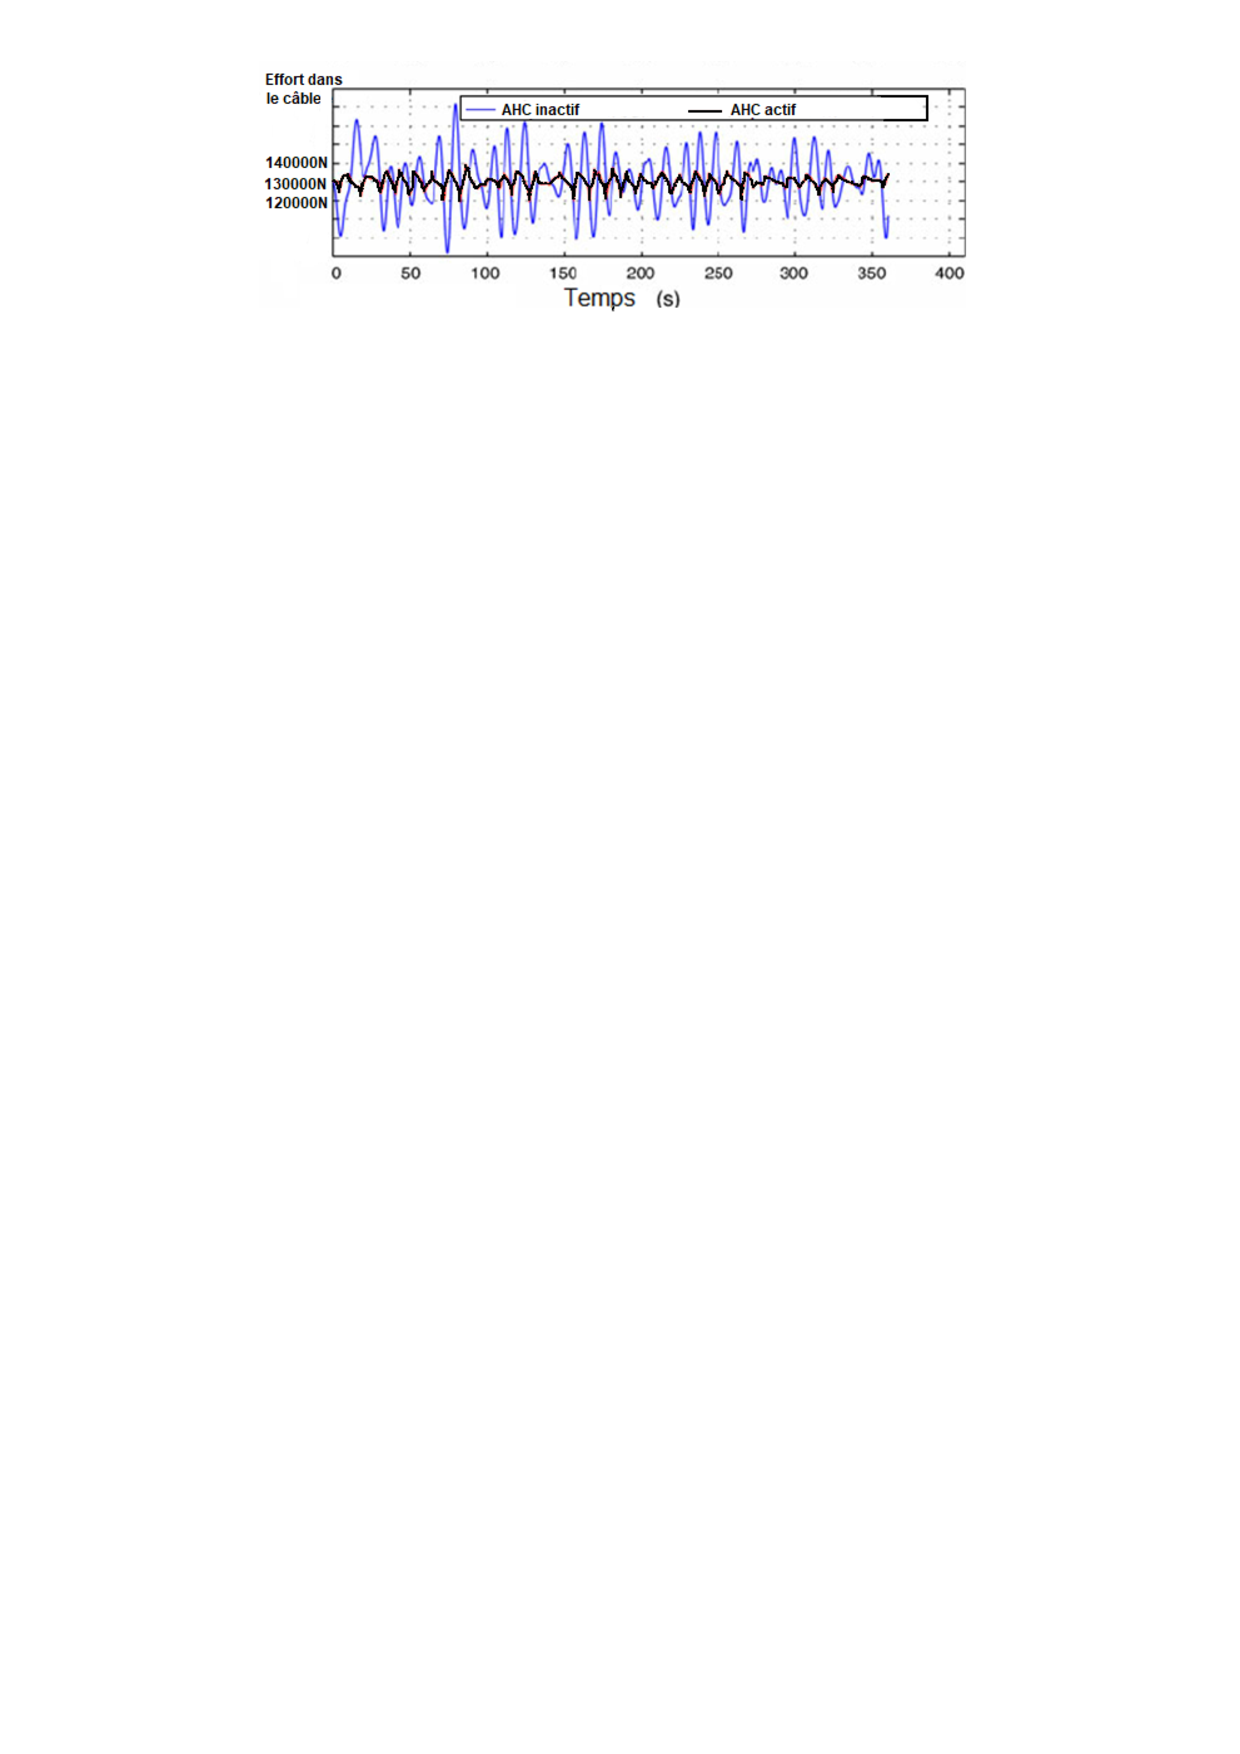
\includegraphics[width=0.75\linewidth]{Fig18}
%\caption{Essai en conditions réelles du système actif}
%\label{Fig18}
%\end{figure}
%\fi
%
%
%
%\question{Appliquer le théorème de la résultante dynamique au ROV en projection sur l’axe vertical ascendant
%et en déduire la relation entre $T(t)$, action du câble sur le ROV, la masse $M_{\text{ROV}}$ du ROV, $g$, l’accélération de la pesanteur, et $\Delta \ddot y(t)$, l’accélération du ROV sur l’axe vertical ascendant. \textit{On pourra montrer que $M\ddot{y}(t)=-Mg+T(t)=T_0\sin\left(\omega t\right)$.}}
%\ifprof
%\begin{corrige}
%%\textbf{Q23}   
%On applique le principe fondamental de la dynamique au ROV en projection suivant $\overrightarrow{y_0}$, on obtient :
%$$M\ddot y(t)=-Mg+T(t)=T_0\sin(\omega t).$$
%
%\end{corrige}
%\else
%\fi
%
%
%\question{Déterminer analytiquement l’expression de $\Delta y(t)$ en fonction de $M_{\text{ROV}}$, masse du ROV et $\omega$, pulsation de la houle. Les constantes d’intégration seront considérées nulles et on prendra {$g = 10 \ \text{m}\cdot \text s^{-2}$}. Calculer la pulsation $\omega$ exprimée en $\text{rad}\cdot \text s^{-1}$ et conclure quant au respect de l’exigence Id 1.1 du cahier des charges pour cet
%essai.}
%\ifprof
%\begin{corrige}
%%\textbf{Q24}   
%On intègre deux fois l'équation précédente et on obtient (avec constantes d'intégrations nulles) :
%$$y(t)=-\dfrac{T_0}{M\omega^2}\sin(\omega t).$$
%
%Soit $y_{\text{max}}=T_0/(M\omega^2)=5500/13000\times(T_p/(2\pi))^2\approx 0,97 < 1$ m . Le cahier des charges est respecté pour cet essai.\\
%
%
%\end{corrige}
%\else
%\fi
%
%
%\section{Conclusion sur la problématique}
%
%\question{La validation des performances de l’AHC à partir de la mesure expérimentale de la \autoref{Fig18}  est-elle
%suffisante ? Une réponse justifiée et argumentée est attendue. Dans le cas d’une réponse négative, une démarche permettant la validation de l’exigence Id 1.1 est attendue.}
%
%\ifprof
%\begin{corrige}
%%\textbf{Q25}   
%Pour la pulsation $\omega=2\pi/T_p=0,66$ rad/s, l'atténuation de 14 dB est vérifié. Il faudrait faire d'autres essais \`a des fréquences comprises entre 0,5 et 1,7 rad/s pour vérifier le CdC.
%
%\end{corrige}
%\else
%\fi

\ifprof
\else
\ifcolle
\else
\begin{tabular}{|p{.95\linewidth}|}
\hline
\begin{enumerate}
\item  $G_{\text{dB}}(\omega)=20\log \left \vert \dfrac{Y_S(j\omega)}{Y_{\text{vague}}(j\omega)}\right \vert$ et 
$G_{\text{dB}(\omega)}<20 \log \dfrac{1}{5}\approx - 14 \ \text{dB} \ \ \forall \ \ \omega\in[0,5;1,7]  \ \text{rad/s}$.
\item ...
\item $K_1=\dfrac{SrP_{G0}}{V_{G0}}$ et $\tau=\dfrac{V_{G0}}{rP_{G0}C_{qR}}.$
\item $\tau=\tau_1+\dfrac{\beta}{\gamma K_1}$, $\omega_n=\sqrt{\frac{\gamma K_1}{\alpha}}$; $\zeta=\dfrac{1}{2}\dfrac{\beta+\gamma K_1 \tau_1}{\sqrt{\alpha \gamma K_1}}.$
\item .
\item .
\item PHC4.
\end{enumerate}\\
\hline
\end{tabular}
\fi % FI COLLE
\fi
\ifprof
\else
\end{multicols}
\fi
